  %  \nonstopmode
\documentclass[10pt,letterpaper,cm]{nupset}
\usepackage[margin=1in]{geometry}
\usepackage{graphicx}
\usepackage{enumerate}
\usepackage{enumitem}
\usepackage{float}
\usepackage{quiver}
\usepackage{amsfonts}
\usepackage{amssymb}
\usepackage{mathtools}
\usepackage{upgreek}
\usepackage{comment}
\usepackage{pgfplots}
\pgfplotsset{compat=1.13}
\usepackage{amsmath,amsthm}
\usepackage{tikz-cd}
\usetikzlibrary{knots,calc, shadows}
\usepackage{xcolor}
\usepackage{soul}
\usepackage{MnSymbol}
\usepackage{extpfeil}
\usetikzlibrary{decorations.markings}
\usetikzlibrary{backgrounds,fit}
\usepackage{faktor}
\usepackage{xfrac}

\usepackage{ mathrsfs }
\usepackage{hyperref}
\usepackage{scrextend}
\hypersetup{colorlinks=true, linkcolor=red,          % color of internal links (change box color with linkbordercolor)
    citecolor=green,        % color of links to bibliography
    filecolor=magenta,      % color of file links
    urlcolor=cyan           }
\usepackage{adjustbox}
\usepackage{media9}
\usepackage{spectralsequences}
\usepackage{thmtools}
\usepackage[capitalise]{cleveref} 
    
\theoremstyle{definition}
\newtheorem{defn}{Definition}[subsection]
\newtheorem{exmp}[defn]{Example}
\newtheorem{non-exmp}[defn]{Non-example}
\newtheorem{note}[defn]{Note}
\newtheorem*{warning}{Warning}

\theoremstyle{theorem}
\newtheorem{theorem}[defn]{Theorem}
\newtheorem{lemma}[defn]{Lemma}
\newtheorem{prop}[defn]{Proposition}
\newtheorem{corollary}[defn]{Corollary}
\newtheorem{claim}[defn]{Claim}
\newtheorem{exercise}[defn]{Exercise}

\theoremstyle{remark}
\newtheorem{remark}[defn]{Remark}
\newtheorem*{todo}{To do}
\newtheorem*{question}{Question}
\newtheorem*{conv}{Convention}
\newtheorem*{aside}{Aside}
\newtheorem*{plan}{Plan}
\newtheorem*{notation}{Notation}
\newtheorem*{term}{Terminology}
\newtheorem*{background}{Background}
\newtheorem*{further}{Further reading}
\newtheorem*{sources}{Sources}

\makeatletter
\def\th@plain{%
  \thm@notefont{}% same as heading font
  \itshape % body font
}
\def\th@definition{%
  \thm@notefont{}% same as heading font
  \normalfont % body font
}
\makeatother


\makeatletter
\renewcommand*\env@matrix[1][*\c@MaxMatrixCols c]{%
  \hskip -\arraycolsep
  \let\@ifnextchar\new@ifnextchar
  \array{#1}}
\makeatother
\pgfplotsset{unit circle/.style={width=4cm,height=4cm,axis lines=middle,xtick=\empty,ytick=\empty,axis equal,enlargelimits,xmax=1,ymax=1,xmin=-1,ymin=-1,domain=0:pi/2}}

\newcommand{\eval}{\mathsf{eval}}
\DeclareMathOperator{\Ima}{Im}
\newcommand{\A}{\mathcal A}
\newcommand{\C}{\mathbb C}
\newcommand{\E}{\vec E}
\newcommand{\PL}{\mathsf{PL}}
\newcommand{\CP}{\mathbb{CP}}
\newcommand{\F}{\mathcal F}
\newcommand{\G}{\vec G}
\renewcommand{\H}{\mathbb H}
\newcommand{\HP}{\mathbb HP}
\newcommand{\K}{\mathbb K}
\DeclareMathOperator{\Ll}{\mathbb L}
\newcommand{\N}{\mathbb N}
\newcommand{\OP}{\mathbb OP}
\renewcommand{\P}{\mathcal P}
\newcommand{\Q}{\mathbb Q}
\newcommand{\U}{\mathcal U}
\newcommand{\I}{\mathbb I}
\DeclareMathOperator{\R}{\mathbb{R}}
\newcommand{\RP}{\mathbb{RP}}
\renewcommand{\S}{\mathbb S}
\newcommand{\T}{\mathcal T}
\newcommand{\X}{\mathbf X}
\newcommand{\Z}{\mathbb Z}
\newcommand{\1}{\mathbb{1}}
\newcommand{\ds}{\displaystyle}
\newcommand{\ran}{\right>}
\newcommand{\lan}{\left<}
\newcommand{\bmat}[1]{\begin{bmatrix} #1 \end{bmatrix}}
\renewcommand{\a}{\vec{a}}
\renewcommand{\b}{\vec b}
\renewcommand{\c}{\mathcal{C}}
\newcommand{\cf}{\mathscr{C}}
\renewcommand{\d}{\mathcal{D}}
\newcommand{\e}{\mathcal{E}}
\newcommand{\h}{\vec h}
\newcommand{\f}{\mathscr{F}}
\newcommand{\g}{\vec g}
\renewcommand{\i}{\vec i}
\renewcommand{\j}{\mathcal{J}}
\renewcommand{\k}{\vec k}
\newcommand{\n}{\mathcal{N}}
\newcommand{\p}{\vec p}
\newcommand{\q}{\vec q}
\newcommand{\m}{\mathcal{M}}
\renewcommand{\r}{\vec r}
\newcommand{\s}{\vec s}
\renewcommand{\t}{\vec t}
\renewcommand{\u}{\vec u}
\newcommand{\w}{\mathscr{W}}
\newcommand{\x}{\vec x}
\newcommand{\dgca}{\mathsf{dgca}}
\newcommand{\dg}{\mathsf{dg}}
\newcommand{\y}{\vec y}
\newcommand{\z}{\vec z}
\newcommand{\0}{\vec 0}
\newcommand{\pt}{\mathsf{pt}}
\newcommand{\from}{\longleftarrow}
\newcommand{\intprodl}{%
    \mathbin{\scalebox{1.5}{$\lrcorner$}}%
}
\newcommand{\intprodr}{%
    \mathbin{\scalebox{1.5}{$\llcorner$}}%
}
\DeclareMathOperator*{\Span}{span}
\DeclareMathOperator{\rng}{range}
\DeclareMathOperator{\gemu}{gemu}
\DeclareMathOperator{\almu}{almu}
\DeclareMathOperator{\id}{id}
\DeclareMathOperator{\tr}{Tr}
\DeclareMathOperator{\fr}{Fr}
\DeclareMathOperator{\fun}{Fun}
\DeclareMathOperator{\tor}{Tor}
\DeclareMathOperator{\im}{im}
\DeclareMathOperator{\ft}{ft}
\DeclareMathOperator{\stab}{Stab}
\DeclareMathOperator{\homeo}{Homeo}
\DeclareMathOperator{\GL}{GL}
\DeclareMathOperator{\SL}{SL}
\DeclareMathOperator{\charr}{char}
\DeclareMathOperator{\norm}{N}
\DeclareMathOperator{\aut}{Aut}
\DeclareMathOperator{\Int}{Int}
\DeclareMathOperator{\ho}{Ho}
\DeclareMathOperator{\ext}{Ext}
\DeclareMathOperator{\Or}{O}
\DeclareMathOperator{\Un}{U}
\DeclareMathOperator{\SO}{SO}
\DeclareMathOperator{\M}{\mathcal{M}}
\DeclareMathOperator{\supp}{supp}
\DeclareMathOperator{\cl}{cl}
\DeclareMathOperator{\wotimes}{\mathbin{\widetilde{\otimes}}}
\DeclareMathOperator{\dom}{dom}
\DeclareMathOperator{\rnk}{rank}
\DeclareMathOperator{\Hom}{Hom}
\DeclareMathOperator{\Alt}{Alt}
\DeclareMathOperator{\dr}{dR}
\DeclareMathOperator{\nil}{\mathsf{Nil}}
\DeclareMathOperator{\nilp}{nilp}
\DeclareMathOperator{\ed}{End}
\DeclareMathOperator{\BM}{BM}
\DeclareMathOperator{\ob}{ob}
\DeclareMathOperator{\ab}{ab}
\DeclareMathOperator{\eq}{eq}
\DeclareMathOperator{\coeq}{coeq}
\DeclareMathOperator{\clength}{cup{-}length}
\DeclareMathOperator{\sgn}{sgn}
\DeclareMathOperator{\orb}{Orb}
\DeclareMathOperator{\cyl}{Cyl}
\DeclareMathOperator{\rel}{rel}
\DeclareMathOperator{\cat}{cat}
\DeclareMathOperator{\op}{op}
\DeclareMathOperator{\sh}{Sh}
\DeclareMathOperator{\ia}{\mathit{IA}}
\DeclareMathOperator{\Gd}{Gd}
\DeclareMathOperator{\coker}{coker}
\DeclareMathOperator{\cocone}{cocone}
\DeclareMathOperator{\map}{Map}
\DeclareMathOperator{\sing}{Sing}
\DeclareMathOperator{\Op}{\mathbf{Op}}
\DeclareMathOperator{\colim}{colim}
\DeclareMathOperator{\hocolim}{hocolim}
\DeclareMathOperator{\holim}{holim}
\DeclareMathOperator{\tot}{Tot}
\DeclareMathOperator{\const}{const}
\DeclareMathOperator{\mor}{Mor}
\DeclareMathOperator{\mc}{MC}
\DeclareMathOperator{\ce}{CE}
\DeclareMathOperator{\B}{\mathcal{B}}
\DeclareMathOperator{\Et}{\acute{E}t}
\DeclareMathOperator{\ch}{\mathbf{Ch}}
\DeclareMathOperator{\vf}{\mathscr{X}}
\DeclareMathOperator{\lb}{\mathcal{LB}}

\newextarrow{\xbigtoto}{{20}{20}{20}{20}}
   {\bigRelbar\bigRelbar{\bigtwoarrowsleft\rightarrow\rightarrow}}

\makeatletter
% the contents of \squarecorner were mostly stolen from pgfmoduleshapes.code.tex
\def\squarecorner#1{
    % Calculate x
    %
    % First, is width < minimum width?
    \pgf@x=\the\wd\pgfnodeparttextbox%
    \pgfmathsetlength\pgf@xc{\pgfkeysvalueof{/pgf/inner xsep}}%
    \advance\pgf@x by 2\pgf@xc%
    \pgfmathsetlength\pgf@xb{\pgfkeysvalueof{/pgf/minimum width}}%
    \ifdim\pgf@x<\pgf@xb%
        % yes, too small. Enlarge...
        \pgf@x=\pgf@xb%
    \fi%
    % Calculate y
    %
    % First, is height+depth < minimum height?
    \pgf@y=\ht\pgfnodeparttextbox%
    \advance\pgf@y by\dp\pgfnodeparttextbox%
    \pgfmathsetlength\pgf@yc{\pgfkeysvalueof{/pgf/inner ysep}}%
    \advance\pgf@y by 2\pgf@yc%
    \pgfmathsetlength\pgf@yb{\pgfkeysvalueof{/pgf/minimum height}}%
    \ifdim\pgf@y<\pgf@yb%
        % yes, too small. Enlarge...
        \pgf@y=\pgf@yb%
    \fi%
    %
    % this \ifdim is the actual part that makes the node dimensions square.
    \ifdim\pgf@x<\pgf@y%
        \pgf@x=\pgf@y%
    \else
        \pgf@y=\pgf@x%
    \fi
    %
    % Now, calculate right border: .5\wd\pgfnodeparttextbox + .5 \pgf@x + #1outer sep
    \pgf@x=#1.5\pgf@x%
    \advance\pgf@x by.5\wd\pgfnodeparttextbox%
    \pgfmathsetlength\pgf@xa{\pgfkeysvalueof{/pgf/outer xsep}}%
    \advance\pgf@x by#1\pgf@xa%
    % Now, calculate upper border: .5\ht-.5\dp + .5 \pgf@y + #1outer sep
    \pgf@y=#1.5\pgf@y%
    \advance\pgf@y by-.5\dp\pgfnodeparttextbox%
    \advance\pgf@y by.5\ht\pgfnodeparttextbox%
    \pgfmathsetlength\pgf@ya{\pgfkeysvalueof{/pgf/outer ysep}}%
    \advance\pgf@y by#1\pgf@ya%
}
\makeatother

\pgfdeclareshape{square}{
    \savedanchor\northeast{\squarecorner{}}
    \savedanchor\southwest{\squarecorner{-}}

    \foreach \x in {east,west} \foreach \y in {north,mid,base,south} {
        \inheritanchor[from=rectangle]{\y\space\x}
    }
    \foreach \x in {east,west,north,mid,base,south,center,text} {
        \inheritanchor[from=rectangle]{\x}
    }
    \inheritanchorborder[from=rectangle]
    \inheritbackgroundpath[from=rectangle]
}

\tikzset{commutative diagrams/.cd,
mysymbol/.style={start anchor=center,end anchor=center,draw=none}
}
\newcommand\MySymb[2][\alpha]{%
  \arrow[mysymbol]{#2}[description]{#1}}

\newcommand{\bi}{\begin{itemize}}
\newcommand{\ei}{\end{itemize}}

\newcommand{\be}{\begin{enumerate}}
\newcommand{\ee}{\end{enumerate}}

\newcommand{\bmp}{\begin{mathpar}}
\newcommand{\emp}{\end{mathpar}}

\newcommand{\bigzero}{\mbox{\normalfont\Large\bfseries 0}}
\newcommand{\rvline}{\hspace*{-\arraycolsep}\vline\hspace*{-\arraycolsep}}

\setlength{\parindent}{0pt}


\newcommand{\mathcolorbox}[2]{\colorbox{#1}{$\displaystyle #2$}}

\newlist{steps}{enumerate}{1}
\setlist[steps, 1]{label = Step \arabic*:}

\pagestyle{headings}

\linespread{1.3}

% info for header block in upper right hand corner
\name{Perry Hart}
\class{MATH 8360}
\assignment{Fall 2021}

\begin{document}
\thispagestyle{empty}
\begin{abstract}
These notes are based on Alexander Voronov's lectures for the course ``Rational Homotopy Theory'' at UMN. Any mistake in what follows is my own.
\end{abstract}

\tableofcontents
\newpage

\section{Introduction} 

\subsection{Lecture 1}

In algebraic topology, we want to associate to any topological space $X$ an algebraic object $A(X)$ such that the mapping $A$ is homotopy invariant, i.e.,
\[
X \sim Y \implies A(X) \sim A(Y).
\]
In an ideal world, we have a converse so that we can learn everything about $X$ by computing $A(X)$. Indeed, topology is hard, and algebra is easy. In reality, however, we can just learn \emph{something} about $X$ from $A(X)$.

\begin{exmp}
If $\widetilde{H}_0(X) =0$, then $X$ is path connected. (Of course, the converse also holds.)
\end{exmp}

In rational homotopy theory (RHT), the mapping $A$ is invariant under \textit{rational equivalence}, i.e.,
\[
X \overset{\Q}{\sim} Y \implies A(X) \cong A(Y).
\] The reverse implication holds under certain assumptions, e.g., that $X$ and $Y$ are simply connected. The object $A(X)$ is pretty simple, a differential graded-commutative algebra (DGCA) over $\Q$.

\begin{exmp} The so-called Sullivan picture of $A$ has the following properties.  
\be
\item $A(S^3) = \Q\left[g_3\right], \ \left\lvert{g_3}\right\rvert =3, \ d{g_3} \equiv 0$. 

Hence $A(S^3)$ is the exterior algebra $\Q \oplus \Q{g_3}$ with $d=0$.
\item $A(S^4) = \Q\left[g_4, g_7\right], \ d{g_4} \equiv 0, \ d{g_7} \equiv g_4^2$.
\ee
\end{exmp}

Moreover, there exists a ``Koszul-dual'' picture of Quillen models used to define $A$. This deals with differential graded-Lie algebras (DGLA's) along with $L_{\infty}$-algebras. (This picture appears to be new for a course on RHT.)

\medskip

We plan to cover the following topics, time permitting.
\be
\item DGCA's
\item model categories
\item simplicial sets
\item polynomial de Rham algebras
\item spectral sequences
\item Quillen models ($L_{\infty}$-versions)
\item Mysterious Duality between physics and math via RHT
\ee

Here are a few good references for these topics.

\bi
\item Bousfield, A. K.; Gugenheim, V. K. A. M. \textit{On PL de Rham theory and rational homotopy type}.
\item F\'{e}lix, Y.; Halperin, S.; Thomas, J.-C. \textit{Rational homotopy theory}.
\item Julian Holstein's online notes  \textit{Rational homotopy theory}.
\ei

\bigskip

First, let's review some concepts and facts from homotopy theory.  Any based space $\left(X_,x\right)$ gives rise to the following algebraic objects.

\bi
\item the graded-abelian group $H_{\bullet}(X;\Z)$
\item the graded-commutative algebra $H^{\bullet}(X;\Z)$
\item for any integer $n>0$, the group $\pi_n(X,x)$ of homotopy components
\item the pointed set $\pi_0(X,x)$ of path components
\ei

We call $\pi_1(X,x)$ the fundamental group and $\pi_n(X,x)$ a higher homotopy group when $n\geq 2$.

\medskip

For any subspaces $A \subset X$ and $B\subset Y$, we have the set  
\[
 \left[\left(X,A\right), \left(Y,B\right)\right]
 \] of homotopy classes of maps $\left(X,A\right)\to \left(Y,B\right)$ of pairs, i.e., maps $f:X \to Y$ such that $f(A) \subset B$. A homotopy between two such maps is an ordinary homotopy $H: X \times I \to Y$ between them such that $H(a,t) \in B$ for any $\left(a,t\right) \in A \times I$. 

\begin{defn}
For any $\left(X,x\right) \in \mathsf{Top}_{\ast}$ and integer $n\geq 1$, define the \textit{$n$-th homotopy group $\pi_n(X,x)$} as the set
\[
\underbrace{\left[\left(I^n, \partial{I^n}\right), \left(X,x\right)\right]}_{\left[\left(S^n, N\right), \left(X,x\right)\right]}
\] equipped with the binary operation
\[
\left(f\ast g\right)(t_1, \ldots, t_n) \equiv 
\begin{cases}
g(t_1, \ldots, t_{n-1}, 2t_n) & t_n \leq \frac{1}2{}
\\ f(t_1, \ldots, t_{n-1}, 2t_n -1) & t_n \geq \frac{1}{2}
\end{cases}
,\] i.e., concatenation in the last variable.
\end{defn}

The Eckmann-Hilton argument tells us
\be
\item that we obtain the same group law by concatenating in any other variable and
\item that $\pi_n$ is abelian when $n\geq 2$.
\ee


\subsection{Lecture 2}

\begin{defn}
A map $f: X \to Y$ is a \textit{weak \emph{(}homotopy\emph{)} equivalence \emph{(}w.e.\emph{)}} if  the induced map
\[
\pi_n(f) : \pi_n(X,x) \to \pi_n(Y,f(x))
\] is an isomorphism for every $n \geq 0$ and $x\in X$.
\end{defn}

Is it cheating to replace homotopy equivalence (h.e.) with w.e.? Not quite, in the following sense.

\begin{theorem}[Whitehead]\label{Whitehead}
Any w.e. between CW complexes is a h.e.
\end{theorem}

Recall that a CW complex is a space of the form $\bigcup_{n\geq {-1}}X^n = \colim_n{X^n}$ where $X^{-1} \equiv \emptyset$ and $X^n$ is obtained from $X^{n-1}$ by adjoining $n$-cells. In other words, $X^n$ is precisely the pushout

\[
\begin{tikzcd}
	{\coprod_{i\in I}S^{n-1}} & {X^{n-1}} \\
	{\coprod_{i\in I}D^n} & {X^n}
	\arrow["\lrcorner"{anchor=center, pos=0.125, rotate=180}, draw=none, from=2-2, to=1-1]
	\arrow[hook', from=1-1, to=2-1]
	\arrow["f", from=1-1, to=1-2]
	\arrow[from=1-2, to=2-2]
	\arrow[from=2-1, to=2-2]
\end{tikzcd},
\] where $f$ denotes the attaching map. In concrete form, $X^n = X^{n-1} \cup_f \left(\coprod_{i\in I}D^n\right)$.

\begin{note}\label{warn}
The CW complexes $S^3 \times \RP^2$ and $\RP^3 \times S^2$ have isomorphic homotopy groups but are \emph{not} weakly equivalent.
\end{note}
\begin{proof}
The  double cover $\Z_2 \to S^n \to \RP^n$ induces a LES
\[\begin{tikzcd}
	\cdots & {\pi_k(\Z_2)} & {\pi_k(S^n)} & {\pi_k(\RP^n)} \\
	& {\pi_{k-1}(\Z_2)} & \cdots & {\pi_0(\RP^n)}
	\arrow[from=1-1, to=1-2]
	\arrow[from=1-2, to=1-3]
	\arrow[from=1-3, to=1-4]
	\arrow[from=1-4, to=2-2]
	\arrow[from=2-2, to=2-3]
	\arrow[from=2-3, to=2-4]
\end{tikzcd}.\]
If $n\geq 2$, then we deduce that the higher homotopy groups of $\RP^n$ are isomorphic to those of $S^n$, so that
\[
\pi_k(\RP^n) = \begin{cases}
0 & k= 0
\\ \Z_2 & k=1 
\\ \pi_k(S^n) & k\geq 2
\end{cases}
.\]
This means that $S^3 \times \RP^2$ and $\RP^3 \times S^2$ have the same homotopy groups. 

\medskip

At the same time, they have different cohomology algebras over $\Z_2$.
\begin{align*}
H^{\bullet}(S^3 \times \RP^2; \Z_2) & \cong \Z_2\left[\xi\right] \otimes \faktor{\Z_2\left[x\right]}{\left(x^3\right)}, \ \left\lvert{\xi}\right\rvert = 3, \ \left\lvert{x}\right\rvert = 1
\\ & \not \cong H^{\bullet}(\RP^3 \times S^2; \Z_2)
\end{align*}
Thus, they are not homotopy equivalent, hence not weakly equivalent, by \cref{Whitehead}.
\end{proof}

\begin{theorem}[CW approximation]\label{CWapprox}
For any space $X$, there is some CW complex $Z$ along with a weak equivalence $Z \xrightarrow{\textit{w.e.}} X$.
\end{theorem}

\Cref{CWapprox} means that the category of spaces localized at weak equivalences is equivalent to the category of CW complexes localized at homotopy equivalences. The category of CW complexes with homotopy classes of maps is called the \textit{homotopy category of spaces}.

\begin{theorem}\label{easier}
Suppose that $f: X \to Y$ is a map of connected CW complexes that induces isomorphisms on $\pi_1({-})$ and $H_n({-};\Z)$ for all $n\geq 2$. Then $f$ is a weak equivalence (hence homotopy equivalence). 
\end{theorem}
\begin{proof}[Idea of proof]
Look at the homotopy fiber of $f$ (also called the \textit{mapping cocone} of $f$):
\[\begin{tikzcd}
	{\cocone(f)} & {E_f} & X \\
	& {Y^I} & Y \\
	\ast & Y
	\arrow[from=1-1, to=3-1]
	\arrow[from=3-1, to=3-2]
	\arrow[from=1-1, to=1-2]
	\arrow["{\eval_1}", from=2-2, to=3-2]
	\arrow[from=1-2, to=1-3]
	\arrow["\lrcorner"{anchor=center, pos=0.125}, draw=none, from=1-1, to=2-2]
	\arrow["\lrcorner"{anchor=center, pos=0.125}, draw=none, from=1-2, to=2-3]
	\arrow["f", from=1-3, to=2-3]
	\arrow["{\eval_0}", from=2-2, to=2-3]
	\arrow[from=1-2, to=2-2]
\end{tikzcd}.\]   The space $E_f$ is homotopy equivalent to $X$. Now apply the Hurewicz theorem to $\cocone(f)$.
\end{proof}

\medskip

Let's now turn to a basic concept of RHT: \textit{rationalization}.

\begin{defn}
We say that a path connected space $X$ is \textit{rational} if $H_n(X;\Z)$ is a $\Q$-vector space for all $n\geq 1$.
\end{defn}

\begin{exmp}\label{circrat}
We construct the space $S^1_{\Q}$ as the colimit of the following sequence 
\[
X_1 \hookrightarrow X_2 \hookrightarrow \cdots \hookrightarrow X_k \hookrightarrow X_{k+1} \hookrightarrow \cdots 
\] in $\mathsf{Top}_{\ast}$. Let $X_1 = \left(S^1, 1\right)$. For any $k\geq 1$, define $w_k : S^1 \to S^1$ by $z \mapsto z^k$ and let $W_k$ denote the pointed mapping cylinder of $w_k$.  Also, define the embeddings
\begin{align*}
s_k & : S^1 \hookrightarrow W_k, \ z \mapsto \left(z,1\right)
\\ t_k & : S^1 \hookrightarrow W_k, \ z \mapsto \left[\left(z,0\right)\right].
\end{align*}
Finally, for each $k\geq 2$, define $X_k$ inductively as the pushout
\[\begin{tikzcd}
	{S^1} & {W_k} \\
	{W_{k-1}} \\
	{X_{k-1}} & {X_k}
	\arrow[from=3-1, to=3-2]
	\arrow["{t_{k-1}}"', from=1-1, to=2-1]
	\arrow[from=2-1, to=3-1]
	\arrow["{s_k}", from=1-1, to=1-2]
	\arrow[from=1-2, to=3-2]
	\arrow["\lrcorner"{anchor=center, pos=0.125, rotate=180}, draw=none, from=3-2, to=1-1]
\end{tikzcd} .\]

Note that $X_n \overset{\text{h.e.}}{\sim} S^1$ for all $n\geq 1$. It turns out, however, that the colimit 
\[
X \coloneqq \colim_n{X_n} = \bigcup_nX_n
\] is the Eilenberg-MacLane space $K(\Q,1)$.
\end{exmp}




\subsection{Lecture 3}

We have maps out of $S^1$ into all finite stages of $S^1_{\Q}$.

\[\begin{tikzcd}
	{X_1} & \cdots & {X_k} & {X_{k+1}} & \cdots \\
	&& {S^1}
	\arrow[hook, from=1-1, to=1-2]
	\arrow[hook, from=1-2, to=1-3]
	\arrow[hook, from=1-3, to=1-4]
	\arrow[hook, from=1-4, to=1-5]
	\arrow["{\underbrace{i_1}_{\id_{S^1}}}", from=2-3, to=1-1]
	\arrow["{i_k}"', from=2-3, to=1-3]
	\arrow["{i_{k+1}}"', from=2-3, to=1-4]
\end{tikzcd}\]

It's easy to see that $X_k \sim S^1$ for all $k\geq 1$, so that $\pi_1(X_k) \cong \Z$.  The inclusion $X_{k-1} \to X_k$, however, induces the mapping 
\begin{align*}
\Z & \to \Z
\\ 1 & \mapsto k \cdot 1
\end{align*} on $\pi_1$.

\begin{claim}
All higher homology groups of $X$ vanish.
\end{claim}
\begin{proof}
Let $n\in \Z_{\geq 2}$. Any map $\Delta^n \to X$ factors through $X_k$ for some $k$ because $\Delta^n$ is compact. Thus, any singular $n$-cycle $\sigma$ in $X$ will be a cycle in $X_k$, which is homotopy equivalent to $S^1$. This means that  $\sigma $ will be a boundary in $X_k$ and thus in $X$. Thus, $H_n(X;\Z) =0$.
\end{proof}

Consider the loop $\gamma : S^1 \xrightarrow{i_1} X_1 \hookrightarrow X$ in $X$. Its homotopy class is nontrivial, for otherwise there is a null-homotopy $S^1 \times I \to X$ factoring through some $X_k$. Since $X_k \sim S^1$, this would imply that $S^1$ is contractible, which is false. 

\medskip

Specifically, $\left[\gamma\right] = k!\left[\delta\right]$ where $\left[\delta\right]$ denotes the bottom generator of $\pi_1(X_k)\cong \Z$. In fact, all $\Q$-multiples of $\left[\gamma\right]$ belong to $\pi_1(X,1)$. Further, any map $S^1 \to X$ factors through some $X_k \hookrightarrow X$, so that its homotopy class is a rational multiple of $\left[\gamma\right]$. It follows that $\pi_1(X,1) \cong \Q\left[\gamma\right] \cong \Q$.

\medskip

By the Hurewicz theorem, $H_1(X;\Z) \cong \pi_1(X,1)^{\ab} \cong \Q$. Hence $X$ is rational.  Also, it's path connected, and any map $S^n \to X$ factors through some $X_k \subset X$, where $X^k \sim S^1$. Thus, if $n\geq 2$, then $\pi_n(X, 1) =0$. We conclude that $S^1_{\Q} \cong K(\Q,1)$.

\begin{term}
The space $S^1_{\Q}$ is called the \textit{rationalization} of $S^1$.
\end{term}

\begin{remark}
The same construction can be done for higher spheres and their attaching maps and thus for all CW complexes.
\end{remark}

\begin{defn}\label{ratz} Let $X$ and $Y$ be path connected spaces.
\be
\item A map $f: X \to Y$ is a  \textit{rational equivalence} if the induced map $H_{\bullet}(f) : H_{\bullet}(X;\Q) \to H_{\bullet}(Y;\Q)$ is an isomorphism. 
\item A \textit{rationalization} of $X$ is a rational space $X_{\Q}$ together with a rational equivalence $X \to X_{\Q}$. 
\ee
\end{defn}

\begin{lemma}
The pair $\left(S^1_{\Q}, i_1 :S^1 \to X\right)$ is a rational equivalence. 
\end{lemma}
\begin{proof}
If $n\geq 3$, then 
\begin{align*}
H_n(S^1;\Q) & =0
\\ & = H_n(S^1_{\Q}; \Z) \otimes_{\Z} \Q 
\\ & = H_n(S^1_{\Q};\Q) \tag{UCT}
.\end{align*}
We also have that
\begin{align*}
H_2(S^1_{\Q}; \Q)  
 & = \tor_1(H_1(S_{\Q}^1; \Z), \Q) \tag{UCT}
\\ & = 0 \tag{$\tor_1({-}. \Q) = 0$}
\\ & = H_2(S^1; \Q).
\end{align*}
Finally, we have that
\begin{align*}
H_1(S_{\Q}^1; \Q) & = H_1(S_{\Q}^1; \Z) \otimes_{\Z} \Q \tag{UCT}
\\ & = \Q \otimes_{\Z} \Q 
\\ & = \Q
\\ &=  H_1(S^1;\Q). 
\end{align*}
The final isomorphism is given by
\[
H_1(i_1) : H_1(S^1;\Q) \to H_1(S_{\Q}^1; \Q)
,\]
which sends the generator $\left[\gamma\right] \in H_1(S^1;\Z)$ to its image $\left[\gamma\right]$ as a $\Q$-vector space generator. 
\end{proof}

\begin{theorem}
Every connected CW complex has a rationalization.
\end{theorem}

\begin{defn}
A \textit{rational homotopy type} is the equivalence class of a path connected space under rational equivalence. 
\end{defn}

\begin{exmp}
Consider $\RP^2$. Recall that
\[
H_n(\RP^2; \Q) \cong \begin{cases} \Q & n= 0
\\ 0 &  n > 0
\end{cases}
.\]
Hence $\RP^2 \to \ast$ is a rational equivalence, so that the rational homotopy type of $\RP^2$ is $\left[\ast\right]$. Further, $\ast$ is trivially a rational space. Therefore, it is a rationalization of $\RP^2$. 
At the same time, we have the nontrivial group
\[
\pi_2^{\Q}(\RP^2) \coloneqq \underbrace{\pi_2(\RP^2)}_{\Z} \otimes \Q \cong \Q
.\] Thus, defining rational equivalence in terms of $H_{\bullet}({-};\Q)$ rather than $H_{\bullet}^{\Q}({-})$ was simple, sensible enough.

\medskip

We shall see, though, that $\RP^2$ is problematic for RHT because it's not nilpotent. (It's not useless, being simply connected.) 
\end{exmp}

\subsection{Lecture 4}

\begin{remark}
Recall that $S_{\Q}^1 = \bigcup_{n\geq 1}X_n =  \colim_{n}X_n$ from \cref{circrat}.  This is exactly the homotopy colimit of the sequence
\[
S^1 \xrightarrow{\id} S^1 \xrightarrow{w_2} S^1 \xrightarrow{w_3} S^1 \xrightarrow{} \cdots
.\] Indeed, we have a commutative square
\[
\begin{tikzcd}
	{S^1} & {W_k} \\
	{S^1} & {S^1}
	\arrow["{s_k}", from=1-1, to=1-2]
	\arrow["{\substack{\textit{collapse onto} \\ \textit{bottom}}}", from=1-2, to=2-2]
	\arrow[equal, from=1-1, to=2-1]
	\arrow["{w_k}"', from=2-1, to=2-2]
\end{tikzcd}
,\] so that $s_k$ is the cofibrant replacement of $w_k$. As a result, we see that
\[
\pi_1(S^1_{\Q}) = \colim_n\pi_1(S^1) = \colim\big(\Z \xrightarrow{{-}\cdot 1} \Z \xrightarrow{{-}\cdot 2} \Z \xrightarrow{{-}\cdot 3}  \cdots\big) = \Q
\]
because $\pi_1({-})$ preserves homotopy colimits of connected spaces.
\end{remark}

\medskip

We now turn to viable candidates, particularly the de Rham algebra, for the rational homotopy type of a space.

\be[label=(\arabic*)]
\item For $\mathsf{Top}_{\ast}$ up to w.e., look at $\pi_{\bullet}(X,x)$.
\bi
\item[\textit{Cons:}] 
\item Hard to compute.
\item Fails to determine the weak homotopy type (see \cref{warn}).
\ei
\item If $X$ is path connected, replace $\pi_{\bullet}(X,x)$ with the easier-to-compute $\pi_1(X)$ and $H_n(X;\Z), \ n\geq 2$.
\bi
\item[\textit{Cons:}] 
\item Fails to determine the weak homotopy type.

(If we introduce the coproduct on $H_{\bullet}(X;\Z)$, then we could do better.)
\ei
\item Look at $H^{\bullet}(X;\Z)$, which is more comfortable as a graded-commutative ring.
\bi
\item[\textit{Cons:}] 
\item Fails to determine the weak homotopy type.
\ei
\item Look at the cochain complex $C^{\bullet}(X;\Z)$ equipped with associative cup product.
\bi
\item[\textit{Cons:}] 
\item Huge.
\item Cup product is only homotopy commutative.
\ei
\bi
\item[\textit{Pros:}] 
\item Determines the weak homotopy type once you extend homotopy commutativity to an $E_{\infty}$-structure (Mandell's theorem).
\ei
\item If $X$ is a (smooth) manifold, then look at the de Rham algebra $\left(\Omega^{\bullet}(X), d\right)$.
\bi
\item[\textit{Cons:}] 
\item Huge.
\item Over $\R$ rather than $\Q$ or $\Z$.
\item Defined for manifolds rather than generic spaces.
\ei
\bi
\item[\textit{Pros:}] 
\item Graded commutative on the nose.
\item Above problems can be resolved by RHT.
\item Determines the rational homotopy type.
\ei
Note that $\Omega^{\bullet}(X) = C^{\infty}(S^{\bullet}(T_X^{\ast}\left[{-1}\right])) = C^{\infty}(\bigwedge^{\bullet}T_X^{\ast})$. In local coordinates, the differential \linebreak $d: \Omega^n(X) \to \Omega^{n+1}(X)$ is defined by
\[
d(f(x_1, \ldots, x_m)dx_{i_1}\land \cdots \land dx_{i_n}) = \sum_{j=1}^m \frac{\partial{f}}{\partial{x_j}}dx_j \land dx_{i_1} \land \cdots \land dx_{i_n}, \ \ m \equiv \dim{X}
\] for each $n\geq 0$.
\ee

\section{Dg-commutative algebras}

We want to focus on candidate (5) and create a homotopy theory of DGCA's.

\medskip

Let $k$ be any field. (It's cleaner to assume $\charr(k) \ne 2$, and soon we'll have $\charr(k) =0$ and $k = \Q$.)

\begin{defn}
A \textit{DGCA} (or \textit{dg-commutative algebra} or \textit{differential graded-commutative algebra}) is a (unital) $k$-algebra that is
\be[label=(\alph*)]
\item $\Z$-graded: $A = \bigoplus_{n\in \Z}A^n, \ a \in A^n \implies \left\lvert{a}\right\rvert = n$

\quad \quad \quad \quad \ \ $A^m \otimes A^n \xrightarrow{\textit{mult.}} A^{m+n}, \ \left\lvert{a \cdot b}\right\rvert = \left\lvert{a}\right\rvert + 
\left\lvert{b}\right\rvert$
\item graded-commutative: any two homogeneous elements $a$ and $b$ satisfy the \textit{Koszul rule of signs}, i.e.,
\[
a \cdot b = \left({-1}\right)^{\left\lvert{a}\right\rvert \left\lvert{b}\right\rvert} b \cdot a
.\]
\item equipped with a differential: a  $k$-linear map $d: A \to A$ of degree $1$, i.e., $d: A^n \to A^{n+1}$, such that
\[
d^2 =0, \ d(1) =0, \ \underbrace{d(ab) = \left(da\right)b + \left({-1}\right)^{\left\lvert{a}\right\rvert}a  \left(db\right)}_{\textit{Leibniz rule}} 
.\]
\ee
\end{defn}

\begin{term}
An element $a\in A^n$ is called
$\begin{cases}
\textit{even} & n $ is even$
\\ \textit{odd} & n $ is odd$
\end{cases}.$
\end{term}

\medskip

For any DGCA $\left(A,d\right)$, its cohomology $H^{\bullet}(A, d)$ is a graded-commutative algebra. Conversely, any graded-commutative algebra  may be viewed as a DGCA with $d=0$. It turns out that the de Rham algebra determines not only the de Rham cohomology but also all rational homotopy groups.

\subsection{Lecture 5}

Let's consider a few examples of DGCA's.

\begin{exmp}\label{fstex} $ $
\be[label=(\arabic*)]
\item Any commutative (associative) algebra is a DGCA $A$ with $A =A^0$ and $d=0$.
\item Any graded-commutative algebra $A = \bigoplus_{n\in \Z}A^n$ is a DGCA with $d=0$.
\item The de Rham algebra $\left(\Omega^{\bullet}(X),d\right)$, with $d$ the exterior derivative.
\item Consider the topological $n$-simplex 
\[
\Delta^n \coloneqq \left\{\left(t_0, \ldots, t_n\right) \mid \sum_{i=0}^n t_i= 1, \ t_i \geq 0\right\}.
\] Let $\Omega^{\bullet}_{\PL}(\Delta^n)$ denote the quotient algebra
\[
\Omega^{\bullet}(n) \coloneqq \frac{\Q\left[t_0, t_1, \ldots, t_n, d{t_0}, d{t_1},\ldots, d{t_n}\right]}{\left(\sum_{i=0}^n{t_i} = 1, \ \sum_{i=0}^n d{t_i} =0\right)}, \quad  \ \left\lvert{d{t_i}}\right\rvert = 1, \ \left\lvert{t_i}\right\rvert = 0
\] over $\Q$. Note that 
\begin{align*}
\Omega^0_{\PL}(\Delta^n) & = \frac{\Q\left[t_0, \ldots, t_n\right]}{\left(\left(\sum_{i=0}^n t_i\right) -1 \right)}
\\ \Omega^{\bullet}_{\PL}(\Delta^n) & = \frac{\Omega^0_{\PL}(\Delta^n)\left[d{t_0}, \ldots, d{t_n}\right]}{\left(\sum_{i=0}^n d{t_i}\right)}  
\\ d{t_i}\cdot d{t_j} & = {- d{t_j} \cdot d{t_i}}
.\end{align*}
Define the differential $d$ on $\Omega^{\bullet}(n)$ as the (graded) derivation satisfying
\begin{align*}
d(t_i) &  = d{t_i}
\\  d\left(d{t_i}\right) & = 0.
\end{align*}
It's clear that $d^2 =0$.
By the definition of $d$, we also can verify that
\[
d\big(f(t_0, \ldots, t_n)d{t_{i_1}}\cdots d{t_{i_p}}\big) = \sum_{j=0}^n \frac{\partial{f}}{\partial{t_j}}d{t_j}d{t_{i_1}}\cdots d{t_{i_p}}
.\]
We call $\Omega^{\bullet}(n)$ the algebra of \textit{rational polynomial differential forms on $\Delta^n$}. In particular, we have that
\[
H^p(\Omega^{\bullet}(n), d) = \begin{cases}
\Q & p = 0 
\\ 0 & p \ne 0
\end{cases}
\]
as the affine plane $\left\{\sum_{i=0}^n t_i =1\right\} \supset \Delta^n$ is contractible. 
\ee
\end{exmp}

A \textit{homomorphism $f: A \to B$ of DGCA's} is a mapping that respects grading, multiplication, and differentials. Denote the category of DGCA's over $k$ by $\dgca_k$. This has the category $\dgca_k^{\geq 0}$ of DGCA's over $k$ concentrated in degree $\geq 0$ as a full subcategory. 

\begin{defn}
A morphism $f: A \to B$ of DGCA's is a \textit{quasi-isomorphism} if it induces an isomorphism
\[
H^{\bullet}(f) : H^{\bullet}(A) \xrightarrow{\sim} H^{\bullet}(B)
\] on cohomology.
\end{defn}

Let $V$ be a graded-vector space $\bigoplus_{m\in \Z} V^m$. The \textit{free graded-commutative algebra on $V$} is 
\[
S^{\bullet}(V) \coloneqq \bigoplus_{n\geq 0}S^n(V) = \frac{T^{\bullet}(V)}{\left(v \otimes w - \left({-1}\right)^{\left\lvert{v}\right\rvert \left\lvert{w}\right\rvert} w \otimes v \right)}, \ \quad v, w \in V,
\] where $T^{\bullet}(V)$ denotes the tensor algebra $\bigoplus_{n \geq 0}V^{\otimes n}$ on $V$.

\begin{exmp} 
 Let $\left\langle x_1, \ldots, x_n\right\rangle_k$ denote the graded-vector space over $k$ spanned by elements $x_1, \ldots, x_n$ of chosen degrees, i.e., the direct sum $kx_1 \oplus \cdots \oplus kx_n$. The polynomial algebra
$k\left[x_1, \ldots, x_n\right]$ is precisely the free algebra $S(\left\langle x_1, \ldots, x_n\right\rangle_k)$.
\end{exmp}

\smallskip

Consider a cochain complex $\left(V = \bigoplus_{m \in \Z}V^m, d\right)$. The \textit{free DGCA $\left(S^{\bullet}(V), d\right)$ on the complex $V$} has differential
\[
d(v_1\cdots v_n) \equiv \sum_{i=1}^n \left({-1}\right)^{\epsilon_i} v_1 \cdots v_{i-1}d{v_i}\cdot v_{i+1}\cdots v_n
, \ \quad \epsilon_i \equiv \sum_{k=1}^{i-1}\left\lvert{v_k}\right\rvert
\] (which arises directly from the Leibniz rule). 


\begin{lemma}
Let $V$ be the cohain complex
\[
0 \xrightarrow{} \underbrace{\Q^n}_{\deg 0} \xrightarrow{\id} \underbrace{\Q^n}_{\deg 1} \xrightarrow{} 0
.\] Then $\Omega^{\bullet}(n) = \left(S^{\bullet}(V), d\right)$.
\end{lemma}
\begin{proof}
Notice that
\begin{align*}
\Omega(n) & =  \frac{\Q\left[t_0, t_1, \ldots, t_n, d{t_0}, d{t_1},\ldots, d{t_n}\right]}{\left(\sum_{i=0}^n{t_i} = 1, \ \sum_{i=0}^n d{t_i} =0\right)}
\\ & \cong \Q\left[t_1, \ldots, t_n, d{t_1}, \ldots, d{t_n}\right], \ d(t_1) \equiv d{t_i}, \ d(d{t_i}) \equiv 0
\end{align*}
as $t_0 = 1 - t_1 - \cdots - t_n$ and $d{t_0} = {-d{t_0} - \cdots - d{t_n}}$. This algebra is clearly isomorphic to $S^{\bullet}(V)$ with $V$ written as
\[
0 \xrightarrow{} \Q t_1 \oplus \cdots \oplus \Q t_n \xrightarrow{d} \Q d{t_1} \oplus \cdots \oplus \Q dt_n \xrightarrow{} 0
.\] 
\end{proof}

\smallskip

The forgetful functor $\dgca_k \xrightarrow{U} \mathsf{dgVect}_k$ into cochain complexes (forgetting multiplication) is right adjoint to the free DGCA functor $\left(V, d\right) \mapsto \left(S(V),d\right)$. This generalizes the familiar adjunction
\[\begin{tikzcd}
	{\mathsf{gca}_k} & { \mathsf{gVect}_k}
	\arrow[""{name=0, anchor=center, inner sep=0}, "S", curve={height=-15pt}, from=1-2, to=1-1]
	\arrow[""{name=1, anchor=center, inner sep=0}, "U", curve={height=-15pt}, from=1-1, to=1-2]
	\arrow["\dashv"{anchor=center, rotate=-90}, draw=none, from=1, to=0]
\end{tikzcd}
.\]

\begin{defn}
A DGCA $\left(A,d\right)$ is \textit{semifree} if $\left(A,0\right)$ is free, i.e., there exists a graded-vector space $V$ such that $S(V) \cong A$.
\end{defn}

\medskip

\begin{defn}[Augmented DGCA]
An \textit{augmentation} on  a DGCA $A$ over $k$ is a homomorphism $\epsilon : A \to k$.
\end{defn}

This is similar to a choice of basepoint of a space. We call the maximal ideal $m \coloneqq \ker{\epsilon}$ the \textit{augmentation ideal} of $A$ and the quotient $\faktor{m}{m^2}$ the \textit{space of indecomposables}.

\begin{note}
There is a split SES 
\[\begin{tikzcd}
	0 & m & A & k & 0
	\arrow[from=1-1, to=1-2]
	\arrow[from=1-2, to=1-3]
	\arrow[from=1-3, to=1-4]
	\arrow[from=1-4, to=1-5]
	\arrow["{\substack{\textit{unit} \\ 1 \leftmapsto 1}}", curve={height=-12pt}, from=1-4, to=1-3]
\end{tikzcd}\] of graded-vector spaces, which induces a sequence
\[
\begin{tikzcd}
	0 & k & A & m & 0 \\
	&&&& {\faktor{m}{m^2}}
	\arrow[two heads, from=1-4, to=2-5]
	\arrow[from=1-4, to=1-5]
	\arrow[from=1-3, to=1-4]
	\arrow[from=1-2, to=1-3]
	\arrow[from=1-1, to=1-2]
\end{tikzcd}
.\]
\end{note}

We can form the category $\dgca/k$ with DGCA morphisms that respect augmentation. This is the slice category of $\dgca_k$ over $k$.

\subsection{Lecture 6}

We now turn to minimal models. The de Rham algebra $\left(\Omega^{\bullet}(X), d\right)$ for a manifold $X$ is too large, whereas the cohomology $H^{\bullet}_{\dr}(X)$ is too small from the RHT perspective. Minimal models lie between these two pictures in a certain sense.

\begin{defn} Let $A$ be a DGCA.
\be 
\item We say that $A$ is \textit{connected} if 
\be
\item $A = A^{\geq 0} \coloneqq \bigoplus_{n \geq 0} A^n$ and
\item the map $k \to A^0$ given by $1 \mapsto 1$ is an isomorphism. 
\ee
\item We say that $A$ is \textit{simply connected} if $A$ is connected and $A^1 =0$.
\ee
\end{defn}

Any connected DGCA $A$ is augmented. Indeed, the subalgebra $A^+ \coloneqq \bigoplus_{n>0}A^n$ is a maximal ideal, and we have an augmentation $A \to \faktor{A}{A^+} = A^0 =k$. Here the augmentation ideal $m$ is precisely $A^+$.

\begin{exmp}
Recall that $\Omega(n) = \Q\left[t_1, \ldots, t_n, d{t_1}, \ldots, d{t_n}\right]$. This is augmented by the mapping
\begin{align*}
\epsilon : \quad t_i & \mapsto 0
\\ d{t_i} &  \mapsto 0, 
\end{align*}
which is the same as the augmentation
\[
f(t_1, \ldots, t_n)d{t_{i_1}} \cdots d{t_{i_p}} \overset{\epsilon}{\longmapsto} \begin{cases}
f(0) & p =0 
\\ 0 & p \geq 1
\end{cases}
.\] The algebra, however, is not connected, for $\Omega(n)^0 = \Q\left[t_1, \ldots, t_n\right] \not\cong \Q$. Even so, it's not simply connected, as 
\[
\Omega(n)^1 = \Q\left[t_1, \ldots, t_n\right] \otimes_{\Q} \underbrace{\left\langle d{t_1}, \ldots, d{t_n}\right\rangle_{\Q}}_{\text{$\Q$-span}} \ne 0 
.\]
Now, the augmentation ideal $m$ is  the homogeneous ideal
\[
\ker{\epsilon} = \left(t_1, \ldots, t_n, d{t_1}, \ldots, d{t_n}\right).
\] This means that the space of indecomposables is the $2n$-dimensional vector space
\begin{align*}
\faktor{m}{m^2} & = \langle t_1, \ldots, t_n, d{t_1}, \ldots, d{t_n}\rangle_{\Q}
\\ & = \underbrace{T_0^{\ast}(T\left[{-1}\right]{\Delta^n})}_{\textit{tangent bundle over $\Delta^n$}}
\end{align*}
 over $\Q$. Here, $T\left[{-1}\right]{\Delta^n}$ denotes the graded-manifold defined by the graded-commutative algebra $\Omega(n)$. (In this sense, we have shifted $\Delta^n$ by ${-1}$.)
\end{exmp}

\begin{defn}\label{sullalg}
A \textit{Sullivan algebra} is a DGCA $S(V)$ for a graded-vector space $V = \bigoplus_{n \geq 1}V^n$ that satisfies the \textit{Sullivan (nilpotent) condition}, i.e., there is a filtration
\[
V(0) \subset V(1) \subset \cdots \subset V(m) \subset V(m+1) \subset \cdots, \ \quad V = \bigcup_{n\geq 0}V(n)
\] of $V$ by graded-vector subspaces (in the sense that $V(m) = \bigoplus_{n\geq 1}\left(V(m) \cap V^n\right)$) such that
\bi
\item $d{V(0)} = 0$ and
\item $d{V(n)} \subset S(V(n-1))$.
\ei 
\end{defn}

\smallskip

Note that a Sullivan algebra is automatically augmented and connected, with 
\begin{align*}
m & = S(V)^+ 
 \coloneqq \bigoplus_{n >0}S(V)^n
\\ &  = S^{\geq 1}(V)
 \coloneqq \bigoplus_{p \geq 1}S^p(V)
\\ \faktor{m}{m^2} & = V
.
\end{align*}


\begin{defn}
A connected DGCA $A$ is \textit{minimal} if $\im{d} \subset \underbrace{\left(A^+\right)^2}_{m^2} $ (i.e., $d$ is decomposable).
\end{defn}

\begin{note}\label{conn}
Let $A= S(V)$. Then $A$ is connected if and only if $V = \bigoplus_{n \geq 1}V^n$, and $A$ is simply connected if and only if $V = \bigoplus_{n \geq 2}V^n$.
\end{note}

\begin{lemma}\label{suffc}
Suppose that a simply connected semifree DGCA $S(V)$ is minimal. Then it's Sullivan. 
\end{lemma}
\begin{proof}
As $S(V)$ is simply connected, \cref{conn} implies that $V = \bigoplus_{n \geq 2} V^n$. For each $m\geq 0$, let 
\[
V(m) = \bigoplus_{n =2}^m V^n,
\]
where $V(0) = V(1) =0$.
The family $\left\{V(m)\right\}_{m \geq 0}$ of graded-subspaces of $V$ is an exhaustive filtration of $V$. As $S(V)$ is minimal, we have that $d{V^n} \subset S^{\geq 1}(V) \cdot S^{\geq 1}(V)$ for every $n \geq 0$. We also have that $d{V^n} \subset S(V)^{n+1}$. It follows that
\[
d{V^n} \subset  \left(S^{\geq 1}(V) \cdot S^{\geq 1}(V)\right) \cap S(V)^{n+1} \subset S\left(\bigoplus_{i=2}^{n-1}V^i\right) = S(V(n-1))
\]  because $V^n \cdot V^i \subset S(V)^{\geq n+2}$ whenever $i\geq 2$. Since $S(V(m-1)) \subset S(V(m))$ for all $m \geq 1$, we conclude that $d{V(n)} \subset S(V(n-1))$. Thus,  $\left\{V(m)\right\}_{m \geq 0}$ satsifies the Sullivan condition.
\end{proof}

\subsection{Lecture 7}


\begin{defn}[Sullivan model] $ $
\be
\item A \textit{Sullivan model of a DGCA $A$} is a Sullivan algebra $S(V)$ together with a quasi-isomorphism \linebreak$S(V) \xrightarrow{\textit{q-iso.}} A$. 
\item A \textit{Sullivan minimal model $M(X)$ of a manifold $X$} is a minimal Sullivan model of $\Omega^{\bullet}(X)$, the de Rham algebra of $X$. (This is defined for ground field $k = \R$.)
\ee
\end{defn}


\begin{exmp}\label{Sull1}
Consider the $n$-sphere $S^n$ where $n\geq 1$. Recall that the cohomology of $\Omega^{\bullet}(S^n)$ is exactly 
\[
H^{\bullet}(S^n; \R) = \faktor{\R\left[\omega\right]}{\left(\omega^2\right)} \cong \R \oplus \R{\omega}, \ \quad  \left\lvert{\omega}\right\rvert \equiv n
\] We want to find a DGCA $M(S^n)$ together with a quasi-isomorphism $M(S^n) \to \Omega^{\bullet}(S^n)$. To begin, define the map 
\begin{align*}
\R\left[x\right] &  \xrightarrow{\varphi} \Omega^{\bullet}(S^n), \ \quad \left\lvert{x}\right\rvert \equiv n, \ d{x} \equiv 0
\\ x & \mapsto \underbrace{\omega \in \Omega^n(S^n)}_{\text{volume form on $S^n$}}, \ \quad d{\omega} =0.
\end{align*}
By construction, this map induces a surjection on cohomology. We must consider two cases.
\bi
\item Suppose that $n$ is odd. Then the degree of $x$ is odd, so that $x^2 =0$. This means that $\R\left[x\right] = \R \oplus \R{x}$, so that  $\varphi$ induces an isomorphism  on cohomology. Thus, $\left(\R\left[x\right], d{x} \equiv 0\right)$ is a Sullivan minimal model of $S^n$. 
\item Suppose that $n$ is even. We want to kill $x^2$ in the  cohomology of $\R\left[x\right]$. To this end, adjoin $y$ to $\R\left[x\right]$ such that $\left\lvert{y}\right\rvert = 2n-1$ and $d{y} = x^2$. Clearly, $x^2$ is killed in cohomology. The map
\begin{align*}
\R\left[x, y\right] &  \xrightarrow{\varphi}  \Omega^{\bullet}(S^n)
\\ x & \mapsto \omega
\\ y & \mapsto 0.
\end{align*} is a morphism of DGCA's.
Since $y$ has odd degree, all higher powers of it are killed in $\R\left[x, y\right]$. Also, $y$ itself is not a cocycle and thus does not affect cohomology. Thus, $\varphi$ induces an isomorphism on cohomology. This means that $\left(\R\left[x,y\right], d{x} \equiv 0, d{y} \equiv x^2\right)$ is a Sullivan model of $S^n$.
\ei
\end{exmp}


\begin{notation} $ $
\be
\item We may write the DGCA $\left(k\left[x_1, \ldots, x_n\right], d{x_1} = 0, d{x_2} = \cdots,  \ldots,  d{x_n} = \cdots\right)$ as 
\[
k\left[x_1, \ldots, x_n \mid d{x_2} = \cdots, \ldots, d{x_n} = \cdots\right].
\]

For example, $M(S^n) = \begin{cases} \R\left[x\right] & \text{$n$ odd} \\ \R\left[x,y \mid d{y} = x^2\right] &  \text{$n$ even} \end{cases}$.
\item We may write the DGCA $k\left[x_1, y_1, x_2, y_2, x_3, x_4, \ldots \mid d{x_1} = y_1, d{x_2} = y_2, d{x_3} = \cdots, d{x_4} = \cdots, \ldots \right]$ as  
\[
k\left[x_1, d{x_1}, x_2, d{x_2}, x_3, x_4, \ldots \mid d{x_3} = \cdots, d{x_4} = \cdots, \ldots\right]
.\]

For example, $\Omega(n) = \Q\left[t_1, \ldots, t_n, d{t_1}, \ldots, d{t_n}\right]$.
\ee
\end{notation}


\begin{note}[Serre]
Recall that $\pi_3(S^2) \cong \Z$. In general, $\pi_{2n -1}(S^n) \otimes_{\Z} \R \cong \R$ when $n$ is even. Further, $\pi_n(S^n) \otimes_{\Z} \R \cong \R$ for all $n \geq 1$. In all other cases, however, $\pi_{\bullet}(S^n)$ is a torsion group.

\medskip

This will be a common pattern for us. The  generators of $\pi_n(X) \otimes \Q$ ($\n \geq 1$) correspond to free generators of $M(X)$.
\end{note}

\begin{exmp}\label{Sull2}
We want to find $M(S^3 \vee S^3)$. The algebra $\Omega^{\bullet}(S^3 \vee S^3)$ consists of pairs $\left(\omega_1, \omega_2\right)$ of differential forms on $S^3$ that agree at the base point. Choose two volume forms $\omega_1$ and $\omega_2$ for the two copies of $S^3$.  Consider the map
\begin{align*}
\R\left[x,y\right] &  \xrightarrow{\psi} \Omega^{\bullet}(S^3 \vee S^3), \ \quad \left\lvert{x}\right\rvert \equiv 3, \ \left\lvert{y}\right\rvert \equiv 3
\\ x & \mapsto \omega_1
\\ y & \mapsto \omega_2.
\end{align*}
The element $xy$ represents a nontrivial cocycle of degree $6$. To kill this in cohomology, adjoin a degree-$5$ variable $z$ to $\R\left[x,y\right]$ such that $d{z} = xy$. We still have nontrivial cocycles $xz$ and $yz$ of degree $8$. Adjoin two degree-$7$ variables $a$ and $b$ such that $d{a} = xz$ and $d{b} = yz$. We can continues this process to infinity to obtain a Sullivan minimal model of $S^3 \vee S^3$. 
\end{exmp}

\begin{remark}
In both \cref{Sull1} and \cref{Sull2}, the minimality of $M(X)$ holds by construction of $d$. Also, $M(X)$ is simply connected unless $X = S^1$, in which case $M(S^1) = \R\left[x\right]$ where $\left\lvert{x}\right\rvert =1$. In this case, let $V(0) = \R{x}$ and $V = V(0)$. Since $d{V(0)} =0$, we see that $M(S^1)$ satisfies the Sullivan condition. Thanks to \cref{suffc}, it follows that $M(X)$ is a Sullivan algebra in all cases.
\end{remark}


\subsection{Lecture 8}

Let us establish a sufficient condition for a DGCA to have a minimal Sullivan model.

\begin{defn}
A $k$-DGCA $A$ is \textit{homologically connected} if $A = \bigoplus_{n \geq 0}A^n$ and $H^0(A) \cong k$. 
\end{defn}


\begin{theorem}\label{minmod}
Every homologically connected DGCA has a minimal Sullivan model. 
\end{theorem}
\begin{proof}
For simplicity, assume that  $A$ is \textit{homologically simply connected}, i.e., it is homologically connected \emph{and} has $H^1(A) =0$. For the general case, see either of the following sources.
\bi
\item \textit{Volume I} of FHT. This uses relative Sullivan models for the proof.
\item  \textit{Volume II} of FHT. This uses structure theory of Sullivan algebras.
\ei
In our case, thanks to \cref{suffc},  it suffices to construct a simply connected minimal model of $A$, i.e.,
\bi
\item a DGCA  $\left(S(V), d\right)$ such that $V = \bigoplus_{n \geq 2}V^n$ and $\im{d} \subset \left(S(V)^+\right)^2$ along with
\item a quasi-isomorphism $\left(S(V), d\right) \xrightarrow{\textit{q-iso.}} \left(A,d\right)$.
\ei 
\begin{plan}
Define $V^n$ and $d\restriction_{S(V^{\leq n})}$ inductively so that $V^1 =0$ and $d{V^n} \subset S(V^{\leq n-1})$. This will imply the minimality condition 
\begin{align*}
d{V^n} \subset S(V^{\leq n-1})^{n+1} \subset S^{ \geq 2}(V^{\leq n-1}) = \left(S(V^{\leq n-1})^+\right)^2
\end{align*}
because $S^{ \geq 2}(V^{\leq n-1}) = V^{ \leq n-1} \cdot S(V^{\leq n-1})^+$. At the same time, define a homomorphism 
\[
f_n : \left(S(V^{\leq n}), d\right) \to \left(A, d\right), \ \quad f_n\restriction_{V^{\leq n-1}} = f_{n-1}\restriction_{V^{ \leq n-1}}
\] such that $H^{\leq n}(f_n)$ is an isomorphism and $H^{n+1}(f_n)$ is an injection. Finally, let $V = \bigoplus_{n \geq 2}V^n$ and \linebreak $f\restriction_{V^n} = f_n\restriction_{V^n}$.
\end{plan}
For our base case, let $V^1 =0$ and define $d = 0$ on $S(\overbrace{V^{\leq1}}^{0}) = k$. Define $f_1 : k \to A$ as the unit map, i.e., the map induced by  the zero map $V^1 \xrightarrow{0} A$.  The map $H^0(f_1)$ is an isomorphism because $H^0(A) \cong k$. Further, the map $H^1(f_1)$ is an isomorphism as the zero map from $0$ to $H^1(A) =0$. Finally, $H^2(f_1)$ is trivially an injective map.

\medskip

For our inductive step, suppose that $n \geq 1$ and that we've constructed $V_n$ and $d$ along with a map $f_n : \left(S(V^{\leq n}), d\right) \to \left(A, d\right)$ inducing an isomorphism on $H^{\leq n}$ and an injection on $H^{n+1}$. Pick cocycles $a_i \in A^{n+1}$ representing a basis of $\coker{H^{n+1}(f_n)}$, so that 
\[
\coker{H^{n+1}(f_n)}= \bigoplus_{i \in I}k\left[a_i\right].
\] 
Likewise, pick cocycles $b_j \in S(V^{\leq n})^{n+2}$ so that 
\[
\ker{H^{n+2}(f_n)} = \bigoplus_{j \in J}k \left[b_j\right]
.\] For each $j\in J$, we may pick $c_j \in A^{n+1}$ such that $f_n(b_j) = d{c_j}$. Now let
\[
V^{n+1} = \left(\bigoplus_{i \in I} k{x_i}\right) \oplus \left(\bigoplus_{j \in J} k{y_j}\right), \ \quad \left\lvert{x_i}\right\rvert = \left\lvert{y_j}\right\rvert = n+1. 
\]
Extend  $d$ to $S(V^{\leq n+1})$ by $d{x_i} \equiv 0$ and $d{y_j} \equiv b_j$, so that $d\restriction_{V^{n+1}}$ takes values in $S(V^{\leq n})^{n+2}$. Since $b_j$ is a cocycle, this extension of $d$ is a differential map.

\medskip

Define $f_{n+1} : V^{\leq n+1} \to A$ by
\begin{align*}
f_{n+1}\restriction_{V^{\leq n}} & = f_n\restriction_{V^{\leq n}}
\\ f_{n+1}(x_i) & = a_i
\\ f_{n+1}(y_j) & = c_j.
\end{align*}

It remains to verify the following two properties. 

\begin{claim} $ $
\be[label=(\arabic*)]
\item $H^{\leq n+1}(f_{n+1})$ is epic.
\item $H^{\leq n+2}(f_{n+1})$ is monic.
\ee
\end{claim}


\subsection{Lecture 9}

\begin{proof} $ $
\be
\item We see that $H^{\leq n+1}(f_{n+1})$  is onto by our construction of $f_{n+1}$. All elements of $H^{n+1}(A)$ missed by $H^{n+1}(f_n)$ are now covered by the $x_i$.
\item The map $H^{\leq n}(f_{n+1})$ is monic as it equals $H^{\leq n}(f_n)$. Further, $H^{n+2}(f_{n+1})$ is monic by construction. No new cocycles are in $S(V^{\leq n+1})^{n+2}$ as compared to $S(V^{\leq n})^{n+2}$. Indeed, 
\[
\label{symme} S(V^{\leq n+1})^{n+2} = S(V^{\leq n})^{n+2}   \tag{$\ast$}
\] 
because $V^1 =0$. Finally, consider the map $H^{n+1}(f_{n+1})$. This may be problematic as we have added cocycles of degree $n+1$, namely the $x_i$.

Let $\left[z\right] \in \ker{H^{n+1}(f_{n+1})}$. We must show that $\left[z\right] =0$. The representative $z$ belongs to $S(V^{\leq n+1})^{n+1}$ and has the form
\[
w + \sum_{i \in I}\lambda_i{x_i} + \sum_{j \in J}\lambda_j{y_j} , \ \quad w\in S(V^{\leq n})^{n+1}
.\] As $z$ is a cocycle, we have that
\begin{align*}
d{z} = 0 & \implies \sum_{j}\lambda_j{b_j} = {-d{w}}
\\ & \implies  \sum_j \lambda_j\left[b_j\right] = 0
\\ & \implies \lambda_j =0 \tag{the $\left[b_j\right]$ linearly independent}
\\ & \implies d{w} = 0.
\end{align*}
Applying $H^{n+1}(f_{n+1})$ to the equation
\[
\left[z\right] = \left[w\right] + \sum_{i \in I}\lambda_i{\left[x_i\right]}  
\] in cohomology
produces
\[
\sum_i \lambda_i\left[a_i\right] = {- H^{n+1}(f_n)(\left[w\right])}
.\] This belongs to $\im{H^{n+1}(f_n)}$. As the $\left[a_i\right]$ are linearly independent, it follows that $\lambda_i = 0$ for all $i$. This means that $z =w$. Hence $z\in S(V^{\leq n})$, and $\left[z\right] \in \ker{H^{n+1}(f_{n})}$. By our induction hypothesis, we conclude that $\left[z\right] =0$.
\ee
\end{proof}
This completes our main proof. Note that equation \eqref{symme}  relies on the fact that $H^1(A) =0$. 
\end{proof}

\bigskip

Let us preview the topic of homotopy theory in $\dgca_{\Q}^{\geq 0}$. Recall the algebra $\Omega^{\bullet}(n)$ from {\cref{fstex}(4)}. We have a tensor product-preserving functor $\Omega({-}) : \mathsf{Top}^{\op} \to \dgca_{\Q}^{\geq 0}$ such that $\Omega(\Delta^n) = \Omega^{\bullet}(n)$. Let $H: X \times I \to Y$ be an ordinary homotopy. We may take its image $\Omega(H) : A \to \Omega(1) \otimes B$ under $\Omega({-})$.

\medskip

Consider the inclusions of endpoints 
\[
\begin{tikzcd}
	{\Delta^0} & {\Delta^1}
	\arrow["{d_0}", shift left=1, from=1-1, to=1-2]
	\arrow["{d_1}"', shift right=1, from=1-1, to=1-2]
\end{tikzcd}
\] in $\Delta^1$. Let $\partial_i = \Omega(d_i)$ for each $i=0,1$.  

\smallskip

We have that $\Omega(0) = \Q$ and
\[
\Omega(1) = \frac{\Q\left[t_0,t_1,d{t_0}, d{t_1}\right]}{\left(t_0 + t_1 = 1, \ d{t_0} + d{t_1} = 0\right)}.
\] Each map $\partial_i: \Omega(1) \to \Q$ is given by
\begin{align*}
\partial_i(d{t_i}) & = 0
\\ \partial_i(t_i) & = 0.
\end{align*}

\begin{defn}
Two maps $f,g : A \to B$ in $\dgca_{\Q}^{\geq 0}$ are \textit{homotopic} if there exists a map $H : A \to \Omega(1) \otimes B$ of DGCA's such that
\begin{align*}
\left(\partial_1 \otimes \id\right) \circ H & = f
\\ \left(\partial_0 \otimes \id\right) \circ H & = g.
\end{align*}
\end{defn}

\begin{exercise}[Homotopy invariance]
If the maps $f$ and $g$ are homotopic, then they induce equal maps on cohomology: $H^{\bullet}(f) = H^{\bullet}(g)$.
\end{exercise}

\section{Model categories}

\subsection{Lecture 10}

\begin{defn}
Let $\c$ be a category. Suppose that the square
\[
\begin{tikzcd}
	U & E \\
	V & B
	\arrow["i"', from=1-1, to=2-1]
	\arrow[from=2-1, to=2-2]
	\arrow["p", from=1-2, to=2-2]
	\arrow[from=1-1, to=1-2]
\end{tikzcd}
\] commutes in $\c$. If there exists a lift $q : V \to E$ for this diagram, then we say that
\bi
\item $i$ has the \textit{left lifting property} (\textit{LLP}) with respect to $p$ and that
\item $p$ has the \textit{right lifting property} (\textit{RLP}) with respect to $i$.
\ei
\end{defn}

\begin{exmp}
Let $\c$ be the category $R\text{-}\mathsf{mod}$ of modules over $R$. 
\bi
\item We say that an object $P$ is \textit{projective} if the unique map $0 \to P$ has the LLP w.r.t. all surjections.
\[
\begin{tikzcd}
	0 & M \\
	P & N
	\arrow[from=1-1, to=2-1]
	\arrow[from=1-1, to=1-2]
	\arrow[two heads, from=1-2, to=2-2]
	\arrow[from=2-1, to=2-2]
	\arrow[dashed, from=2-1, to=1-2]
\end{tikzcd}
\]
\item We say that an object $I$ is \textit{injective} if the unique map $I \to 0$ has the RLP w.r.t. all injections. 
\[
\begin{tikzcd}
	N & I \\
	M & 0
	\arrow[from=1-1, to=1-2]
	\arrow[hook', from=1-1, to=2-1]
	\arrow[from=2-1, to=2-2]
	\arrow[from=1-2, to=2-2]
	\arrow[dashed, from=2-1, to=1-2]
\end{tikzcd}
\]
\ei
\end{exmp}

\begin{defn}
Let  $f : A \to B$ and  $f' : A' \to B'$ be maps in $\c$. We say that $f$ is a \textit{retract} of $f'$ if we can factor the $\id$ morphism
\[
\begin{tikzcd}
	A & A \\
	B & B
	\arrow["\id", from=1-1, to=1-2]
	\arrow["f", from=1-2, to=2-2]
	\arrow["f"', from=1-1, to=2-1]
	\arrow["\id"', from=2-1, to=2-2]
\end{tikzcd}
\] through $f'$ as follows.
\[
\begin{tikzcd}
	A & {A'} & A \\
	B & {B'} & B
	\arrow[from=1-1, to=1-2]
	\arrow[from=1-2, to=1-3]
	\arrow["f"', from=1-1, to=2-1]
	\arrow["{f'}"', from=1-2, to=2-2]
	\arrow["f", from=1-3, to=2-3]
	\arrow[from=2-1, to=2-2]
	\arrow[from=2-2, to=2-3]
	\arrow["\id", curve={height=-12pt}, from=1-1, to=1-3]
	\arrow["\id"', curve={height=12pt}, from=2-1, to=2-3]
\end{tikzcd}
\]
\end{defn}

\begin{defn}
A \textit{(closed) model category} is a category $\m$ equipped with three classes of morphisms closed under composition.
\bi
\item the class $\w$ of \textit{weak equivalences}
\item the class $\f$ of \textit{fibrations}
\item the class $\cf$ of \textit{cofibrations}
\ei
A  map in $\f \cap \w$ is called an \textit{acyclic} or \textit{trivial} fibration. Likewise, a  map in $\cf \cap \w$ is called an \textit{acyclic} or \textit{trivial} cofibration. 

\smallskip

Moreover, $\m$ must satisfy the following five axioms.
\be
\item[(MC1)] It has small limits and colimits, i.e., is complete and cocomplete.
\item[(MC2)] The class $\w$ has the \textit{2-out-of-3} property. For any two morphisms $f$ and $g$ with $fg$ defined, if two of $f$, $g$, and $fg$ belong to $\w$, then so does the third.
\item[(MC3)] The classes $\f$, $\cf$, and $\w$ are all closed under retracts.
\item[(MC4)] Any cofibration has the LLP w.r.t. all acyclic fibrations.

Any acyclic cofibration has the LLP w.r.t. all fibrations. 
\item[(MC5)] Any morphism $f$ in $\m$ can be functorially factored in two ways:
\begin{align*}
f & = pi, \ \quad \text{$p$ acyclic fibration, $i$ cofibration} 
\\ f & = qj, \ \quad  \text{$q$ fibration, $j$  acyclic cofibration} 
.
\end{align*}
\[
 \begin{tikzcd}
	\bullet & \bullet \\
	\bullet & \bullet
	\arrow["f", from=1-1, to=1-2]
	\arrow["g"', from=2-1, to=2-2]
	\arrow[from=1-1, to=2-1]
	\arrow[from=1-2, to=2-2]
\end{tikzcd}  \mapsto 
\begin{tikzcd}
	\bullet & \bullet & \bullet \\
	\bullet & \bullet & \bullet
	\arrow["i", from=1-1, to=1-2]
	\arrow["{i'}"', from=2-1, to=2-2]
	\arrow[from=1-1, to=2-1]
	\arrow[dashed, from=1-2, to=2-2]
	\arrow["{p'}"', from=2-2, to=2-3]
	\arrow["p", from=1-2, to=1-3]
	\arrow[from=1-3, to=2-3]
\end{tikzcd}. \quad \quad \quad \quad 
\]

\ee
\end{defn}

\smallskip

\begin{term} 
Let $X \in \ob{\m}$. We say that
\bi
\item  $X$ is \textit{fibrant} if the unique map $X \to 1$ is a fibration and that
\item $X$ is \textit{cofibrant} if the unique map $0 \to X$ is a cofibration. 
\ei
\end{term}

\begin{exmp}
The category $\mathsf{Top}$ has the structure of a model category. The class $\w$ consists of all weak homotopy equivalences. The class $\f$ consists of all Serre fibrations, maps with the RLP w.r.t. all inclusions of the form 
\[
D \times \left\{0\right\} \hookrightarrow D \times I, \ \quad \text{$D$ an $n$-dimensional ball}.
\] (We could replace balls with CW complexes.) Thus, a map $p$ is a fibration if and only if it has the HLP w.r.t. all balls:
\[
\begin{tikzcd}
	{D\times \left\{0\right\}} & E \\
	{D\times I} & B
	\arrow[hook', from=1-1, to=2-1]
	\arrow[from=1-1, to=1-2]
	\arrow[from=2-1, to=2-2]
	\arrow["p", from=1-2, to=2-2]
	\arrow[dashed, from=2-1, to=1-2]
\end{tikzcd}
.\]
The class $\cf$ must consist of all maps with the LLP w.r.t. Serre fibrations that are weak equivalences. One can prove that $\cf$ equals the class of all retracts of relative CW complexes.  
\end{exmp}

\subsection{Lecture 11}

Let $R$ be a (unital) commutative ring. Consider the category $\dg{\text{-}}R{\text{-}}\mathsf{mod}^{\leq 0}$ of complexes of $R$-modules bounded by zero on the right. This has a model category structure, with
\begin{align*}
\w & = \text{the class of quasi-isos.}
\\ \f & = \text{the class of cochain maps $f$ such that $f_n$ is surjective for all $n<0$}
\\ \cf & =  \text{the class of cochain maps $f$ such that $f_n$ is injective  and $\coker{f_n}$ is a projective module for all $n\leq 0$}
. 
\end{align*}
This is known as the \textit{projective} model category structure on $\dg{\text{-}}R{\text{-}}\mathsf{mod}^{\leq 0}$. All complexes are fibrant, and a complex is cofibrant if and only if it is term-wise projective.

\medskip

Likewise, the category $\dg{\text{-}}R{\text{-}}\mathsf{mod}^{\geq 0}$ has an \textit{injective} model category structure, with
\begin{align*}
\w & = \text{the class of quasi-isos.}
\\ \f & = \text{the class of cochain maps $f$ such that $f_n$ is surjective and $\ker{f_n}$ is an injective module for all $n\geq 0$}
\\ \cf & =  \text{the class of cochain maps $f$ such that $f_n$ is injective $n > 0$}
. 
\end{align*} 
Here a complex is fibrant if and only if it is term-wise injective. 

\medskip

Now consider the category $\dg{\text{-}}R{\text{-}}\mathsf{mod}$ of possibly unbounded complexes. This has a projective model category structure:
\begin{align*}
\w & = \text{the class of quasi-isos.}
\\ \f & = \text{the class of cochain maps $f$ such that $f_n$ is surjective for all $n\in \Z$}
\\ \cf & =  \text{the class of cochain maps that have the LLP w.r.t. all acyclic fibrations}
. 
\end{align*}
A useful description of $\cf$ is much harder in this case. The following sources derive one in detail:
\bi
\item Hovey
\item Dwyer and Spalinski
\item Goerss and Schemmerhorn.
\ei

We can equip $k\text{-}\dgca^{\geq 0}$ with a similar model category structure:
\begin{align*}
\w & = \text{the class of quasi-isos.}
\\ \f & = \text{the class of all maps $f$ such that $f_n$ is surjective for all $n\geq 0$}
\\ \cf & =  \text{the class of all maps that have the LLP w.r.t. all acyclic fibrations}
. 
\end{align*}

\medskip

Let's turn to a few basic properties of model categories.

\begin{lemma}\label{easy}
Suppose that $\m$ is a model category. The cofibrations in $\m$ are precisely the maps with the LLP w.r.t. all acyclic fibrations.
\end{lemma}
\begin{proof}
Suppose that $f: K \to L$ has the LLP w.r.t. all acyclic fibrations. We must show that $f$ is a cofibrations. By MC5, we may factor $f$ as
\[
K \xrightarrow{\substack{i\\ \text{cof.}}} L' \xrightarrow{\substack{p \\ \text{acyclic fib.}}} L
.\] Apply the LLP of $f$ to get a lift $h: L \to L'$ for the commutative sqaure
\[
\begin{tikzcd}
	K & {L'} \\
	L & L
	\arrow["\id"', from=2-1, to=2-2]
	\arrow["f"', from=1-1, to=2-1]
	\arrow["p", from=1-2, to=2-2]
	\arrow["i", from=1-1, to=1-2]
\end{tikzcd}
.\] It's easy to check that
\[
\begin{tikzcd}
	K & K & K \\
	L & {L'} & L
	\arrow["f"', from=1-1, to=2-1]
	\arrow["i"', from=1-2, to=2-2]
	\arrow["f", from=1-3, to=2-3]
	\arrow["\id", from=1-1, to=1-2]
	\arrow["\id", from=1-2, to=1-3]
	\arrow["h"', from=2-1, to=2-2]
	\arrow["p"', from=2-2, to=2-3]
	\arrow["\id"', curve={height=24pt}, from=2-1, to=2-3]
\end{tikzcd}
\] commutes. Hence $f$ is a retract of $i$. By MC3, it follows that $f$ is a cofibration. 
\end{proof}

\begin{remark}
The other three versions of \cref{easy} are true and are proven similarly.
\end{remark}

\begin{corollary} $ $
\be[label=(\arabic*)]
\item Both cofibrations and acyclic cofibrations are stable under pushouts and coproducts.
\[
\begin{tikzcd}
	A & B \\
	C & D
	\arrow["i"', from=1-1, to=2-1]
	\arrow[from=1-1, to=1-2]
	\arrow["j", from=1-2, to=2-2]
	\arrow[from=2-1, to=2-2]
	\arrow["\lrcorner"{anchor=center, pos=0.125, rotate=180}, draw=none, from=2-2, to=1-1]
\end{tikzcd} \ \ \quad \text{$i$ cofibration $\implies$ $j$ cofibration}
\]
\item Both fibrations and acyclic fibrations are stable under pullbacks and pushouts.
\item If $\left(\m ,\w, \f, \cf\right)$ is a model category, then so is $\left(\m^{\op} ,\w^{\op}, \cf^{\op}, \f^{\op}\right)$.
\ee
\end{corollary}


\begin{lemma}\label{clcomp}
Cofibrations are stable under transfinite composition, i.e., for any sequence
\[
X_0 \xrightarrow{\text{cofib.}} X_1 \xrightarrow{\text{cofib.}} X_2 \xrightarrow{\text{cofib.}} \cdots
\] of cofibrations, the map $X_0 \to \colim_{i \geq 0}{X_i}$ is a cofibration.
\end{lemma}

\subsection{Lecture 12}

Consider any model category $\left(\m, \w, \f, \cf\right)$. 

\begin{defn}[Homotopy category]
The \textit{homotopy category} $\ho(\m)$ of $\m$ is the localization $\m\left[\w^{-1}\right]$ w.r.t. the class $\w$ of weak equivalences.
\end{defn}

In general, for any category $\m$ and any class $\w$ of morphisms in $\c$, the localization w.r.t. $\w$ is a category $\m\left[\w^{-1}\right]$ together with a functor $\m \to \m\left[\w^{-1}\right]$ that sends any $w\in \w$ to an isomorphism and satsifies the following universal property. For any functor $\m \to \c$ sending $\w$ to isomorphism in $\c$, there is a unique factorization of the form
\[
\begin{tikzcd}
	\m & {\m\left[\w^{-1}\right]} & \c
	\arrow[from=1-1, to=1-2]
	\arrow["{\exists!}"', dashed, from=1-2, to=1-3]
	\arrow[curve={height=-18pt}, from=1-1, to=1-3]
\end{tikzcd}
.\]

\smallskip

A direct construction is possible (modulo set-theoretic subtleties) as long as $\w$ satisfies properties similar to those for localization of associative rings:

\bi
\item $\w$ is a subcategory (like a multiplicative subset of a ring);
\item the so-called Ore condition. 
\ei
We'll use the specific properties of a model category instead.


\medskip

We now begin developing homotopy theory in model categories. We must generalize the notion of a homotopy $H: X \times I \to Y$ for spaces, where $I = \Delta^1$ or $\left[0,1\right]$. Let $\m$ be a model category, 

\begin{notation} $ $
\bi
\item The symbol $\hookrightarrow$ denotes a cofibration.
\item The symbol $\twoheadrightarrow$ denotes a fibration.
\item The symbol $\xrightarrow{\sim}$ denotes a weak equivalence. 
\ei
\end{notation}

\begin{defn}
Let $A \in \ob{\m}$. A \textit{cylinder object} for $A$ is an object $\cyl(A)$ in $\m$ along with a commutative triangle
\[
\begin{tikzcd}
	{A  \coprod A} & {\cyl(A)} \\
	& A
	\arrow["q"', from=1-2, to=2-2]
	\arrow["i", hook, from=1-1, to=1-2]
	\arrow["\nabla"', from=1-1, to=2-2]
	\arrow["\wr", from=1-2, to=2-2]
\end{tikzcd}
.\]
\end{defn}

Note that cylinders always exist in a model category with $q$ moreover being an acyclic fibration.

\begin{defn}\label{lhom}
A \textit{left homotopy} between maps $f,g: A \to B$  in $\m$ via $\cyl(A)$ is a map $H : \cyl(A) \to B$ such that
\[
\begin{tikzcd}
	{A\coprod A} & {\cyl(A)} \\
	& B
	\arrow["{f+g}"', from=1-1, to=2-2]
	\arrow["i", hook, from=1-1, to=1-2]
	\arrow["H", from=1-2, to=2-2]
\end{tikzcd}
\] commutes. In this case, write $f \overset{\ell}{\sim}g $.
\end{defn}


\begin{defn} $ $
\be
\item Let $A \in \ob{\m}$. A \textit{path space object} for $A$ is an object $A^I$ in $\m$ along with a commutative triangle
\[
\begin{tikzcd}
	{A\times A} & {A^I} \\
	A
	\arrow["\Delta", from=2-1, to=1-1]
	\arrow["\sim"', from=2-1, to=1-2]
	\arrow["r", from=2-1, to=1-2]
	\arrow["p"', two heads, from=1-2, to=1-1]
\end{tikzcd}
.\]
\item A \textit{right homotopy} between maps $f,g: A \to B$ in $\m$ via $B^I$ is a map $H:A \to B^I$ such that
\[
\begin{tikzcd}
	A & {B^I} \\
	& {B\times B}
	\arrow["{\left(f,g\right)}"', from=1-1, to=2-2]
	\arrow["H", from=1-1, to=1-2]
	\arrow["p", two heads, from=1-2, to=2-2]
\end{tikzcd}
\] commutes. In this case, write $f \overset{r}{\sim} g$.
\ee
\end{defn}

\begin{notation}
The expression $f \sim g$ means that $f \overset{\ell}{\sim} g$ and $f \overset{r}{\sim} g$.
\end{notation}

\begin{exmp}
Let $\m = \mathsf{Top}$. We have that $f \overset{\ell}{\sim} g \iff f \overset{r}{\sim} g$ thanks to the natural isomorphism
\[
\Hom(A \times I, B) \cong \Hom(A, B^I), \ \quad B^I = \map(I, B)
\]  in $A$ and $B$.
\end{exmp}

\smallskip

For a notion of homotopy classes of maps in model categories, let
\begin{align*}
\pi^{\ell}(A,B) & = \faktor{\Hom(A,B)}{\overset{\ell}{\sim}}
\\ \pi^{r}(A,B) &= \faktor{\Hom(A,B)}{\overset{r}{\sim}}
.
\end{align*}
These are sets of equivalence classes for the equivalence relations generated by  left and right homotopy. 
\pagebreak
\begin{lemma}\label{props} $ $
\be[label=(\arabic*)]
\item If $f \overset{\ell}{\sim} g : A \to B$, then $hf \overset{\ell}{\sim} hg$ for any map $h : B \to C$.
\item If $C$ is fibrant  and $f \overset{\ell}{\sim} g : B \to C$, then $fk \overset{\ell}{\sim} gk$ for any map $k : A \to B$.
\item If $C$ is fibrant, then we have a well-defined composition map
\begin{align*}
\pi^{\ell}(A,B) \times \pi^{\ell}(B,C) & \to \pi^{\ell}(A,C)
\\ \left(f,g\right) & \mapsto g \circ f.
\end{align*}
\item If $A$ is cofibrant, then left homotopy between maps $A \to B$ is an equivalence relation on $\Hom(A,B)$.
\item If $B$ is cofibrant and $h: X \to Y$ is an acyclic fibration or a weak equivalence between fibrant objects, then the mapping $f \overset{h_{\ast}}{\longmapsto} h \circ f$ induces a bijection
\[
\pi^{\ell}(B,X) \xrightarrow{\cong} \pi^{\ell}(B,Y).
\]
\ee
\end{lemma}
For a proof of this, see Chapter 1 of Hovey.

\subsection{Lecture 13}

Suppose that $\m$ is a model category. We want to study the relationship between left and right homotopy.

\begin{lemma}
Let $A, B \in \ob{\m}$ and $f,g : A \to B$. Suppose that $A$ is cofibrant and that $f \overset{\ell}{\sim} g$. For any path space object $B^I$, we have that $f \overset{r}{\sim} g$ via $B^I$. 
\end{lemma}
\begin{proof}
By assumption, we have a commutative triangle
\[
\begin{tikzcd}
	{A\coprod A} & {\cyl(A)} \\
	& B
	\arrow["{f+g}"', from=1-1, to=2-2]
	\arrow["H", from=1-2, to=2-2]
	\arrow["i", hook, from=1-1, to=1-2]
\end{tikzcd}
.\] We want a commutative triangle of the form
\[
\begin{tikzcd}
	A & {B^I} \\
	& {B\times B}
	\arrow["{\left(f,g\right)}"', from=1-1, to=2-2]
	\arrow[dotted, from=1-1, to=1-2]
	\arrow["p", from=1-2, to=2-2]
\end{tikzcd}
.\]
To this end, construct  the commutative square
\[ \label{lift}
\begin{tikzcd}[column sep=large]
	A & {B^I} \\
	{\cyl(A)} & {B\times B}
	\arrow["{i_0}"', hook', from=1-1, to=2-1]
	\arrow["{r \circ f}", from=1-1, to=1-2]
	\arrow["p", two heads, from=1-2, to=2-2]
	\arrow["{\left(f \circ q, H\right)}"', from=2-1, to=2-2]
\end{tikzcd} \tag{$\ast$}
,\] where $r$ and $q$ are as in the definition of path space object and cylinder object, respectively. We want to find a lift $K : \cyl(A) \to B^I$ for this square. 

\medskip

First, note that $i_0$ is a cofibration as the composition of two cofibrations. Indeed, the inclusion map \linebreak $A \xrightarrow{j_0} A \coprod A$ is a cofibration as a pushout
\[
\begin{tikzcd}
	0 & A \\
	A & {A\coprod A}
	\arrow[hook', from=1-1, to=2-1]
	\arrow[from=1-1, to=1-2]
	\arrow["{j_0}", from=1-2, to=2-2]
	\arrow[from=2-1, to=2-2]
	\arrow["\lrcorner"{anchor=center, pos=0.125, rotate=180}, draw=none, from=2-2, to=1-1]
\end{tikzcd}
\] of the cofibration $0 \to A$. Since $i_0 = i\circ j_0$, this is also a cofibration.  Second, note that $i_0$ is also a weak  equivalence. Indeed, the composite
\[ 
\begin{tikzcd}
	A & {\cyl(A)} & A
	\arrow["{i_0}", from=1-1, to=1-2]
	\arrow["q", from=1-2, to=1-3]
	\arrow["\id"', curve={height=18pt}, from=1-1, to=1-3]
\end{tikzcd}
\] is a weak equivalence, and $q$ is a weak equivalence. Hence $i_0$ is one by the two-out-of-three property. It follows that $i_0$ is an acyclic cofibration. By the LLP, there exists a lift $K : \cyl(A) \to B^I$ for \eqref{lift}.

\medskip

It's easy to check that $K\circ i_1$ is a right homotopy between $f$ and $g$ via $B^I$, i.e., the triangle
\[
\begin{tikzcd}[row sep=large]
	A & {B^I} \\
	& {B\times B}
	\arrow["{K\circ i_1}", from=1-1, to=1-2]
	\arrow["p", from=1-2, to=2-2]
	\arrow["{\left(f,g\right)}"', from=1-1, to=2-2]
\end{tikzcd}
\] commutes. 

\end{proof}

\begin{corollary}
Let $A$ be cofibrant and $B$ be fibrant. 
\be[label=(\arabic*)]
\item Suppose that $f \overset{\ell}{\sim} g$ via a cylinder object $\cyl(A)$. Then $f \overset{r}{\sim} g$ via any path space object $B^I$, and $f \overset{\ell}{\sim} g$ via any cylinder object $\cyl(A)$.  
\item $f \overset{\ell}{\sim} g \iff f \overset{r}{\sim} g$. 
\ee
\end{corollary}

Under these assumptions, the expression $\left[A,B\right]$ will denote $\pi^{\ell}(A,B)$ or $\pi^r(A,B)$ (which are equal).

\begin{theorem}[``Whitehead'']\label{qWhite}
Suppose that both $A$ and $B$ are fibrant and cofibrant. Then a map $f: A \to B$ is a weak equivalence if and only if it is a homotopy equivalence. 
\end{theorem}

For a proof of this, see chapter 1 of Hovey. Note that Whitehead's theorem for CW complexes follows from \cref{qWhite} for the standard model structure on $\mathsf{Top}$. Here, every object is fibrant, and the cofibrant objects are precisely retracts of CW complexes. 

\subsection{Lecture 14}

Let $\m$ be a model category. Recall the economic description of the homotopy category of $\m$:

\[
\ho(\m) = \m\left[\w^{-1}\right], \ \quad \text{$\w$ class of w.e.'s}
.\] We now turn to an alternative description.

\medskip

Let $X \in \ob{\m}$. By MC5, we can factor the map $X \to 1$ as
\[
\begin{tikzcd}
	X & {R{X}} & 1
	\arrow[two heads, from=1-2, to=1-3]
	\arrow["{i_X}", hook, from=1-1, to=1-2]
	\arrow["\sim"', hook, from=1-1, to=1-2]
\end{tikzcd}
\]
and the map $0 \to X$ as
\[
\begin{tikzcd}
	0 & {Q{X}} & X
	\arrow[hook, from=1-1, to=1-2]
	\arrow["{p_X}", two heads, from=1-2, to=1-3]
	\arrow["\sim"', two heads, from=1-2, to=1-3]
\end{tikzcd}
.\] 
 We call $R{X}$ and $Q{X}$ the \textit{fibrant} and \textit{cofibrant replacement} of $X$, respectively. Note that both $R$ and $Q$ are functors $\m \to \m$. Also, they induce natural transformations
 \begin{align*}
 Q  \Rightarrow \id_{\m} &, \ \quad p_X : Q{X}   \xrightarrow{\sim} X
 \\ \id_{\m}  \Rightarrow R &, \ \quad i_X : X  \xrightarrow{\sim} R{X}.
 \end{align*}
Both $QR{X}$ and $RQ{X}$ are fibrant and cofibrant. Indeed, the map $QR{X} \xrightarrow{p_{RX}} R{X} \to 1$ is a fibration as the composition of fibrations. Likewise, the map $0 \to Q{X} \xrightarrow{i_{Q{X}}} RQ{X}$ is a cofibration as the composition of cofibrations. 

\begin{theorem}\label{equivthm}
The functor $RQ : \m \to \m$ induces an isomorphism
\[
\ho(\m) \xrightarrow{\cong} \left(\ob{\m}, \Hom(X,Y) \equiv \left[RQ{X}, RQ{Y}\right]\right)
\] of categories. 
\end{theorem}

By  \cref{qWhite}, we also have an equivalence 
\[
\begin{tikzcd}
	{\left(\text{fibrant cofibrant objects of $\m$},  \left[X,Y\right]\right) } & { \left(\ob{\m},  \left[RQ{X}, RQ{Y}\right]\right)}
	\arrow["i", curve={height=-12pt}, from=1-1, to=1-2]
	\arrow["RQ", curve={height=-12pt}, from=1-2, to=1-1]
\end{tikzcd}
\] of categories where $i$ denotes the inclusion functor.  

\begin{corollary} $ $
\be[label=(\arabic*)]
\item The category $\ho(\mathsf{Top})$ is equivalent to the category of retracts of CW complexes with homotopy classes of maps between CW complexes. (The latter is equivalent to the category of CW complexes with homotopy classes of maps.)
\item The \textit{derived category} of $R$-modules 
\[
D^{\leq 0}(R\text{-}\mathsf{mod}) \coloneqq \ho(\underbrace{\dg{\text{-}}R{\text{-}}\mathsf{mod}^{\leq 0}}_{\substack{\text{proj. model}\\ \text{structure}}}) = \dg{\text{-}}R{\text{-}}\mathsf{mod}^{\leq 0}\left[\textit{q-iso.$^{-1}$}\right]
\]
is equivalent to the category of projective complexes with cochain homotopy classes of cochain maps.
\ee
\end{corollary}

\smallskip

\begin{proof}[Proof sketch of \cref{equivthm}]
Let $\m_{RQ} =  \left(\ob{\m},  \left[RQ{X}, RQ{Y}\right]\right)$. We want to show that $\m_{RQ}$ has the universal property of $\m\left[\w^{-1}\right]$. First, let's show that 
\[
\left(\id_{\ob{\m}}, RQ_{\mor(\m)}\right) : \m \longrightarrow \m_{RQ}
\] takes weak equivalences to isomorphisms. Let $f: X \to Y$ be a w.e. in $\m$. We have a commutative diagram
\[ \label{doubs}
\begin{tikzcd}
	{RQ{X}} & {RQ{Y}} \\
	{Q{X}} & {Q{Y}} \\
	X & Y
	\arrow["{Q{f}}", from=2-1, to=2-2]
	\arrow["f"', from=3-1, to=3-2]
	\arrow["{p_X}"', from=2-1, to=3-1]
	\arrow["{p_Y}", from=2-2, to=3-2]
	\arrow["{RQ{f}}", from=1-1, to=1-2]
	\arrow["{i_{QX}}", from=2-1, to=1-1]
	\arrow["{i_{Q{Y}}}"', from=2-2, to=1-2]
	\arrow["\wr"', from=2-2, to=3-2]
	\arrow["\wr", from=2-1, to=3-1]
	\arrow["\sim", from=3-1, to=3-2]
	\arrow["\wr"', from=2-1, to=1-1]
	\arrow["\wr", from=2-2, to=1-2]
\end{tikzcd} \tag{$\ast$}
.\] By applying the 2-out-of-3 property twice, we see that $RQ{f}$ is a weak equivalence. Hence it is an isomorphism in $\m_{RW}$ by  \cref{qWhite}.

\medskip

Next, let's show that $\m_{RQ}$ has the universal property. Let $\c$ be any category and suppose that $\m \xrightarrow{G} \c$ is any functor taking $\w$ to isomorphims. We must find a unique functor $\widetilde{G} : \m_{RQ} \to \c$ such that 
\[
\begin{tikzcd}
	\m & {\m_{RQ}} \\
	& \c
	\arrow["G"', from=1-1, to=2-2]
	\arrow["RQ", from=1-1, to=1-2]
	\arrow["{\widetilde{G}}", from=1-2, to=2-2]
\end{tikzcd}
\]  commutes. Define $\widetilde{G}$ on objects by $X \mapsto G(X)$.   Consider any homotopy class of the form $\left[f\right] : RQ{X} \to RQ{Y}$. Define the map $\widetilde{G}(\left[f\right])$ as follows.
\[
\begin{tikzcd}
	X & Y \\
	{Q{X}} & {Q{Y}} \\
	{RQ{X}} & {RQ{Y}}
	\arrow["\wr", from=2-1, to=1-1]
	\arrow["\wr"', from=2-1, to=3-1]
	\arrow["f"', from=3-1, to=3-2]
	\arrow["\wr", from=2-2, to=3-2]
	\arrow["\wr"', from=2-2, to=1-2]
\end{tikzcd}
\ \ \overset{G}{\longmapsto}  \ \
\begin{tikzcd}
	X & Y \\
	{GQ{X}} & {GQ{Y}} \\
	{GRQ{X}} & {GRQ{Y}}
	\arrow["\cong", from=2-1, to=1-1]
	\arrow["\cong"', from=2-1, to=3-1]
	\arrow["{G(f)}"', from=3-1, to=3-2]
	\arrow["\cong", from=2-2, to=3-2]
	\arrow["\cong"', from=2-2, to=1-2]
	\arrow["{\widetilde{G}(\left[f\right])}", dashed, from=1-1, to=1-2]
\end{tikzcd}
.\]
Now, by applying $G$ to a diagram like \eqref{doubs}, we see that $G(h) = \widetilde{G}(RQ{h})$ for any map $h : X \to Y$ in $\m$.

\medskip

It remains to show that $\widetilde{G}(\left[f\right])$ (equivalently, $G(f)$) is independent of the choice of representative $f$.

\subsection{Lecture 15}

\begin{claim}
Let $f,g : A \to B$ be maps in $\m$. If $f \overset{\ell}{\sim} g$ (or $f \overset{r}{\sim} g$)  in $\m$, then $G(f) = G(g)$.
\end{claim}
\begin{proof}
Suppose that $f \overset{\ell}{\sim} g$. This gives us a homotopy
\[
\begin{tikzcd}
	{A\coprod A} & {\cyl(A)} \\
	& B
	\arrow["{f+g}"', from=1-1, to=2-2]
	\arrow[from=1-1, to=1-2]
	\arrow["H", from=1-2, to=2-2]
\end{tikzcd}
.\] We also have commutative diagrams
\[
\begin{tikzcd}[row sep = large]
	A & {A\coprod A} & B && A & {A\coprod A} & B \\
	& {\cyl(A)} &&&& {\cyl(A)} \\
	{}
	\arrow[from=1-1, to=1-2]
	\arrow["{f+g}", from=1-2, to=1-3]
	\arrow["f", curve={height=-24pt}, from=1-1, to=1-3]
	\arrow[from=1-2, to=2-2]
	\arrow["{i_0}"', from=1-1, to=2-2]
	\arrow["H"', from=2-2, to=1-3]
	\arrow["{i_1}"', from=1-5, to=2-6]
	\arrow[from=1-6, to=2-6]
	\arrow["H"', from=2-6, to=1-7]
	\arrow[from=1-5, to=1-6]
	\arrow["{f+g}", from=1-6, to=1-7]
	\arrow["g", curve={height=-24pt}, from=1-5, to=1-7]
\end{tikzcd}
.\] Note that $q\circ i_0 = q \circ i_1 = \id_A$, where $q$ is a weak equivalence. Hence
\[
 G(w)G(i_0) = G(w) G(i_1) = \id_{G(A)},
\] and $G(w)$ has an inverse. This implies that $G(i_0) = G(i_1)$, so that
\[
G(f) = G(H)G(i_0) = G(H)G(i_1) = G(g).
\]
\end{proof}

This completes our main proof.
\end{proof}

In summary, the homotopy category $\ho(\m)$ is characterized as either $\m\left[\w^{-1}\right]$ or $\left(\ob{\m},  \left[RQ{-}, RQ{-}\right]\right)$. We'll mostly use the latter as it's easier to work with.

\bigskip

We now want to develop homological algebra in model categories. Suppose that $F: \m \to \n$ is a functor between model categories. This induces a functor $\ho(\m) \to \ho(\n)$ whenever $F$ preserves weak equivalences. Usually, however, this is too strong a condition. To find weaker conditions, we should look at Quillen adjunctions.

\begin{defn}
An adjoint pair $\left(F : \m \to \n, G : \n \to \m\right)$ of functors is a \textit{Quillen adjunction} if $F$ preserves cofibrations and $G$ preserves fibrations. In this case, we call $F$ a \textit{left Quillen functor} and $G$ a \textit{right Quillen functor}.
\end{defn}

\begin{note} Consider an adjunction $F \dashv G$. TFAE.
\be
\item The pair $\left(F,G\right)$ is a Quillen adjunction.
\item $F$ preserves both cofibrations and acyclic cofibrations. 
\item $G$ preserves both fibrations and acyclic fibrations. 
\ee
\end{note}

\begin{exmp}
Recall the free-forgetful adjunction 
\[
\begin{tikzcd}
	{ \dg{\text{-}}\mathsf{Vect}_{\Q}^{\leq 0}} & {\dgca_{\Q}^{\geq 0}}
	\arrow[""{name=0, anchor=center, inner sep=0}, "F"', curve={height=12pt}, from=1-1, to=1-2]
	\arrow[""{name=1, anchor=center, inner sep=0}, "U"', curve={height=12pt}, from=1-2, to=1-1]
	\arrow["\dashv"{anchor=center, rotate=90}, draw=none, from=0, to=1]
\end{tikzcd}, \ \quad \left(V,d\right) \mapsto \left(S(V),d\right)
.\] For both of these model categories, $\w$ consists of all quasi-isomorphisms and $\f$ consists of all degree-wise surjective maps. Thus, $\left(F, U\right)$ is a Quillen adjunction because $U$ preserves both fibrations and acyclic fibrations. (In fact, it preserves weak equivalences.)
\end{exmp}

\begin{lemma}\label{induced} $ $
\be
\item Any left Quillen functor $F : \m \to \n$ induces a functor $L{F} : \ho(\m) \to \ho(\n)$, called the \textit{left derived functor} of $F$.
\[
\begin{tikzcd}
	\m & \m & \n & {\ho(\n)} \\
	& {\ho(\m)} & {}
	\arrow["Q", from=1-1, to=1-2]
	\arrow["F", from=1-2, to=1-3]
	\arrow[from=1-3, to=1-4]
	\arrow[from=1-1, to=2-2]
	\arrow["{L{F}}"', dashed, from=2-2, to=1-4]
\end{tikzcd}
\]
\item Dually, any right Quillen functor $G: \n \to \m$ induces a functor $R{G} : \ho(\n) \to \ho(\m)$, called the \textit{right derived functor} of $G$.  
\[
\begin{tikzcd}
	\n & \n & \m & {\ho(\m)} \\
	& {\ho(\n)} & {}
	\arrow["R", from=1-1, to=1-2]
	\arrow["G", from=1-2, to=1-3]
	\arrow[from=1-3, to=1-4]
	\arrow[from=1-1, to=2-2]
	\arrow["{R{G}}"', dashed, from=2-2, to=1-4]
\end{tikzcd}
\]
\ee
\end{lemma}

\subsection{Lecture 16}

By the universal property of localization, it suffices to show that the composite 
\[
\m \xrightarrow{Q} \m \xrightarrow{F} \n \to \ho(\n)
\]
sends weak equivalences to isomorphisms. Recall that $F$ preserves acyclic cofibrations. Hence the composite $\m \xrightarrow{F} \n \to \ho(\n)$ sends acyclic cofibrations to isomorphisms. 

\begin{lemma}[Ken Brown] \label{KB}
Consider any functor $F : \m \to \c$. Suppose that $F$ sends acyclic cofibrations between cofibrant objects to isomorphisms. Then $F$ sends every weak equivalence between cofibrant objects to an isomorphism. 
\end{lemma}
\begin{proof}
Suppose that $f : A \to B$ is a weak equivalence with both $A$ and $B$ cofibrant. We must show that $F(f)$ is an isomorphism. Form a factorization
\[
\begin{tikzcd}
	{A \coprod B} & C & B
	\arrow["j", hook, from=1-1, to=1-2]
	\arrow["\sim"', two heads, from=1-2, to=1-3]
	\arrow["p", from=1-2, to=1-3]
\end{tikzcd}
\] of $f + \id_B$.  We have that $f = p\circ j \circ i_A$ and $\id_B = p \circ j \circ i_B$, so that
\begin{align*}
F(f) & = F(p) \circ F(j \circ i_A)
\\ F(\id_B) & = F(p) \circ F(j \circ i_B).
\end{align*}
With a ``bootstrap'' method, we can show that each of  $F(j \circ i_B)$, $F(j \circ i_A)$, and $F(p)$ is an isomorphism.  

\medskip

We claim that $j \circ i_B : B \to C$ is an acyclic cofibration between cofibrant objects. We've assumed that $B$ is cofibrant. Note that $i_B$ is a cofibration as the   pushout of $0 \hookrightarrow A$, where $A$ is cofibrant by assumption. As $j$ is also a cofibration, so is $j \circ i_B$ as the composition of two cofibrations. Thus, the composite $0 \hookrightarrow B \xrightarrow{j \circ i_B} C$ is also a cofibration, i.e., $C$ is cofibrant. Further, we have that
\[
\begin{tikzcd}[row sep = huge, column sep=large]
	B & C & B
	\arrow["{j \circ i_B}", hook, from=1-1, to=1-2]
	\arrow["p", from=1-2, to=1-3]
	\arrow["\sim"', from=1-2, to=1-3]
	\arrow["{\id_B}", curve={height=-18pt}, from=1-1, to=1-3]
\end{tikzcd}
\] commutes, so that $j \circ i_B$ is a w.e. by the 2-out-of-3 property. This implies that $F(j \circ i_B)$ is an isomorphism. 

\medskip

Similarly, $j \circ i_A$ is a cofibration between cofibrant objects. Also,  $f = p \circ \left(j \circ i_A\right)$, where $f$ is a weak equivalence. Hence $j \circ i_A$ is acyclic. It follows that $F(j \circ i_A)$ is also an isomorphism. 

\medskip

Finally, since $\id_{F(B)} = F(p) \circ F(j \circ i_B)$, we see that $F(p)$ is an isomorphism. This means that $F(f)$ is an isomorphism as  the composition $F(p) \circ F(j \circ i_A)$ of isomorphisms.  
\end{proof}

It's clear that \cref{induced} follows from \cref{KB} because $Q$ preserves weak equivalences. 

\begin{note}
If a functor $F: \m \to \c$ sends weak equivalences between cofibrant objects to isomorphisms, then we may define the \textit{left derived functor} $L{F} : \ho(\m) \to \c$ of $F$ via $F \circ Q$.
\end{note}

\begin{exmp}
Let $\m =  \dg{\text{-}}R{\text{-}}\mathsf{mod}^{\leq 0}$ with the projective model structure. Let $N$ be an $R$-module. We have a natural bijection
\[
\Hom_R(M^{\bullet} \otimes_R N, K^{\bullet}) \cong \Hom_R(M^{\bullet}, \underline{\Hom}_R(N, K^{\bullet}))
\] in $M^{\bullet}, K^{\bullet} \in \ob{\m}$. Here, $\underline{\Hom}_R(N, K^{\bullet})$ consists of all homogeneous  chain maps of any degree.  The right adjoint $\Hom(N, {-})$, however, fails to preserve fibrations for it's only left exact. This means that the adjunction ${-} \otimes N \dashv \Hom(N, {-})$ is not a Quillen adjunction.

\medskip

If $N$ is projective, then it is a Quillen adjunction. In this case, the right derived functor carries no new information, in the sense that
\[
R{\underline{\Hom}(N, K^{\bullet})} = \underline{\Hom}(N, R{K^{\bullet}}) = \underline{\Hom}(N, K^{\bullet}) 
.\]

\medskip

Suppose that $N$ is arbitrary. We can still define $L\left({-} \otimes N\right)$ by
\[
M^{\bullet} \mapsto M^{\bullet} \overset{\mathbb{L}}{\otimes}_R N \coloneqq Q{M^{\bullet}} \otimes_R N, where
\] $Q{M^{\bullet}}$ is a projective resolution.  In particular, by viewing the $R$-module $M$ as the complex $0 \to M \to 0$, we can define
\[
\tor_{-n}(M,N) = H^n(Q{M} \otimes N).
\]
Likewise, we can define $\ext$ in terms of either $\underline{\Hom}(Q{M}, N)$ or $\underline{\Hom}(N, R{M})$ with the dual model structure. 

\end{exmp}

\subsection{Lecture 17}

Our goal is to prove the main theorem on Quillen adjunctions. 

\begin{theorem}
For any Quillen adjunction
\[
 \begin{tikzcd}
	\m & \n
	\arrow[""{name=0, anchor=center, inner sep=0}, "F"', curve={height=6pt}, from=1-1, to=1-2]
	\arrow[""{name=1, anchor=center, inner sep=0}, "G"', curve={height=6pt}, from=1-2, to=1-1]
	\arrow["\dashv"{anchor=center, rotate=90}, draw=none, from=0, to=1]
\end{tikzcd}
,\] the pair $\left(\Ll{F}, \R{G}\right)$ is an adjoint pair.
\end{theorem}
\begin{proof}
We must exhibit a natural bijection
\[
\Hom_{\ho(\n)}(\Ll{F{A}}, X) \cong \Hom_{\ho(\m)}(A, \R{G{X}})
\] in $A$ and $X$. First, note that the natural transformation $\left\{p_A : Q{A} \xrightarrow{\sim} A\right\}_{A \in \ob{\m}}$ induces a bijection
\[
\Hom_{\ho(\m)}(A, \R{G{X}}) \xrightarrow{p_A^{\ast}} \Hom_{\ho(\m)}(Q{A}, G{R{X}})
\] because $\ho(\m) = \m\left[\w^{-1}\right]$. Likewise, the natural transformation $\left\{i_X : X \xrightarrow{\sim} R{X}\right\}_{X \in \ob{\n}}$ induces a bijection
\[
\Hom_{\ho(\n)}(\Ll{F{A}}, X) \xrightarrow{\left(i_X\right)_{\ast}} \Hom_{\ho(\n)}(F{Q{A}}, R{X})
.\] Next, note that
\[
\Hom_{\ho(\m)}(Q{A}, G{R{X}}) = \left[R{Q{Q{A}}}, R{Q{G{R{X}}}}\right] = \left[Q{A}, G{R{X}}\right]
.\]
 Indeed, the map $\pi^{\ell}(Q{A}, Q{G{R{X}}}) \xrightarrow{p_{\ast}} \pi^{\ell}(Q{A}, G{R{X}})$ is a bijection by \cref{props}(5), and the map \linebreak $\pi^{r}(Q{A}, Q{G{R{X}}}) \xrightarrow{p^{\ast}} \pi^{r}(Q{Q{A}}, Q{G{R{X}}})$ is a bijection by the dual of \cref{props}(5). These bijections arise from the commutative square
 \[
 \begin{tikzcd}
	{Q{Q{A}}} & {Q{G{R{X}}}} \\
	{Q{A}} & {G{R{X}}}
	\arrow["\wr"', two heads, from=1-1, to=2-1]
	\arrow["\wr", two heads, from=1-2, to=2-2]
	\arrow[from=2-1, to=1-2]
	\arrow[dashed, from=2-1, to=2-2]
	\arrow[dashed, from=1-1, to=1-2]
\end{tikzcd}
. \] The two $R's$ are attached in a similar way. Moreover, we have a similar identification
\[
\Hom_{\ho(\n)}(F{Q{A}}, R{X}) = \left[F{Q{A}}, R{X}\right].
\]
\medskip

It suffices to show that $F \dashv G$ induces a natural bijection $\left[F{Q{A}}, R{X}\right] \cong \left[Q{A}, G{R{X}}\right]$. 
\begin{lemma}\label{cof-fib}
If $B$ is cofibrant and $Y$ fibrant, then the bijection $\Hom_{\m}(B, G{Y}) \xrightarrow{\left({-}\right)^{\#}} \Hom_{\n}(F{B}, Y)$ induces a bijection $\left[B, G{Y}\right] \xrightarrow{\cong} \left[F{B}, Y\right]$.
\end{lemma}
\begin{proof}
It suffices to show that
\be[label=(\alph*)]
\item $f \overset{\ell}{\sim} g \implies f^{\#} \overset{\ell}{\sim} g^{\#}$ and
\item $f^{\#} \overset{r}{\sim} g^{\#} \implies f \overset{\ell}{\sim} g$.
\ee
For (a), suppose that we have a homotopy of the form
\[
\begin{tikzcd}
	{B \coprod B} & {\cyl(B)} \\
	& {G{Y}}
	\arrow["{f+g}"', from=1-1, to=2-2]
	\arrow["H", from=1-2, to=2-2]
	\arrow[hook, from=1-1, to=1-2]
\end{tikzcd}
.\] This gives rise to a commutative triangle
\[
\begin{tikzcd}
	{F(B \coprod B)} & {F{\cyl(B)}} \\
	& Y
	\arrow["{\left(f+g\right)^{\#}}"', from=1-1, to=2-2]
	\arrow["{H^{\#}}", from=1-2, to=2-2]
	\arrow[hook, from=1-1, to=1-2]
\end{tikzcd}
.\] We claim that this is a homotopy from $f^{\#}$ to $g^{\#}$. Since $F$ preserves coproducts as a left adjoint, it suffices to show that $F{\cyl(B)}$ is a cylinder object for $F{B}$. Note that $\cyl(B)$ is cofibrant and that $F$ preserves weak equivalences between cofibrant objects by our proof of \cref{KB}. Thus, we have that
\[
\begin{tikzcd}
	{B\coprod B} & {\cyl(B)} \\
	& B
	\arrow["\nabla"', from=1-1, to=2-2]
	\arrow["\wr", from=1-2, to=2-2]
	\arrow[hook, from=1-1, to=1-2]
\end{tikzcd} 
\overset{F}{\longmapsto}
\begin{tikzcd}
	{F{B}\coprod F{B}} & {F{\cyl(B)}} \\
	& {F{B}}
	\arrow["\nabla"', from=1-1, to=2-2]
	\arrow["\wr", from=1-2, to=2-2]
	\arrow[hook, from=1-1, to=1-2]
\end{tikzcd}
.\] This means that $F{\cyl(B)}$ is a cylinder object for $F{B}$.
\end{proof} 
Taking $Q{A}$ for $B$ and $R{X}$ for $Y$ completes our main proof.
\end{proof}

\subsection{Lecture 18}

\begin{defn}
A Quillen adjunction $F \dashv G$ is a \textit{Quillen equivalence} if the pair $\left(\Ll{F}, \R{F}\right)$ is an equivalence $\ho(\m) \simeq \ho(\n)$ of categories. 
\end{defn}

Our big goal is to establish a Quillen equivalence like $\mathsf{Top}^{\Q} \xrightarrow{\sim} \dgca_{\Q}^{\geq 0}$.

\bigskip

Let's look at homotopy (co)limits in a model category $\m$. We have all (co)limits in $\m$ by MC1. How do they descend to $\ho(\m)$? In $\mathsf{Top}$, pushouts fails to respect weak equivalences. For example, the disk $D^2$ is contractible, but the pushouts
\[
\begin{tikzcd}
	{S^1} & \ast && {S^1} & {D^2} \\
	\ast & \ast && \ast & {\frac{D^2 \coprod \ast}{S^1 \sim \ast}}
	\arrow[from=1-1, to=2-1]
	\arrow[from=1-1, to=1-2]
	\arrow[from=2-1, to=2-2]
	\arrow[from=1-2, to=2-2]
	\arrow[from=1-4, to=2-4]
	\arrow[from=1-4, to=1-5]
	\arrow[from=1-5, to=2-5]
	\arrow[from=2-4, to=2-5]
	\arrow["\lrcorner"{anchor=center, pos=0.125, rotate=180}, draw=none, from=2-5, to=1-4]
	\arrow["\lrcorner"{anchor=center, pos=0.125, rotate=180}, draw=none, from=2-2, to=1-1]
\end{tikzcd}
\] are not homotopy equivalent, as the latter is equivalent to $S^2$. In general, we can fix this problem by ``deriving'' (co)limits just as we derived Quillen adjunctions by $\left(F, G\right) \mapsto \left(\Ll{F}, \R{G}\right)$. To this end, recall the following facts of category theory.

\begin{prop}
Let $\c$ be a (co)complete category and $\j$ be a small category. Consider the category $\fun(\j, \c)$ of $\j$-shaped diagrams in $\c$. Let $\const : \c \to \fun(\j, \c)$ denote the constant-diagram functor. We have adjunctions
\begin{align*}
\colim_{\j} & \dashv \const
\\ \const & \dashv \lim_{\j}
.\end{align*}
\end{prop}

The natural bijections
\begin{align*}
\Hom_{\c}(\colim_{\j}{F}, C) & \cong \Hom_{\fun(\j, \c)}(F, \const_C)
\\ \Hom_{\fun(\j, \c)}(\const_C, F) &  \cong \Hom_{\c}(C, \lim_{\j}{F})
\end{align*}
are precisely the universal properties of $\colim_{\j}{F}$ and $\lim_{\j}{F}$, respectively. 


\medskip

We want to take $\Ll{\colim_{\j}}$ and $\R{\lim_{\j}}$ for the homotopy colimit and limit, respectively, provided that 
\bi
\item $\c$ has a model structure,
\item $\fun(\j, \c)$ has a suitable model structure, and
\item both $\left(\colim_{\j}, \const\right)$ and $\left(\const, \lim\right)$ are Quillen adjunctions under these two model structures. 
\ei
In this case, let $\hocolim_{\j} = \Ll{\colim_{\j}}$ and $\holim_{\j} = \R{\lim_{\j}}$. For example, $\fun(\j, \c)$ has a suitable model structure when $\c$ is a \textit{combinatorial} model category. 

\begin{defn}[Homotopy pushout]
Consider any span $\begin{tikzcd}
	C & A & B
	\arrow["g"', from=1-2, to=1-1]
	\arrow["f", from=1-2, to=1-3]
\end{tikzcd}$
in a model category. Factor the composite $Q{A}\to  A \xrightarrow{f} B$ as $Q{A} \hookrightarrow \widetilde{B} \overset{\sim}{\twoheadrightarrow} B$. Likewise, factor $Q{A} \to A \xrightarrow{g} C$   as
$Q{A} \hookrightarrow \widetilde{C} \overset{\sim}{\twoheadrightarrow} C$. Now take the ordinary pushout
\[
\begin{tikzcd}
	{Q{A}} & {\widetilde{B}} \\
	{\widetilde{C}} & H
	\arrow[hook, from=1-1, to=1-2]
	\arrow[hook', from=1-1, to=2-1]
	\arrow[from=2-1, to=2-2]
	\arrow[from=1-2, to=2-2]
	\arrow["\lrcorner"{anchor=center, pos=0.125, rotate=180}, draw=none, from=2-2, to=1-1]
\end{tikzcd}
\] as the homotopy pushout  of our span.
\end{defn}

\begin{exmp}
Let $\m = \mathsf{Top}$. Let $f: A \to B$ be a map of spaces. We can factor $f$ as
\[
\begin{tikzcd}
	A & {M{f}} & B
	\arrow["\sim", from=1-2, to=1-3]
	\arrow["i_1",hook, from=1-1, to=1-2]
\end{tikzcd}
\]
where $M{f}$ denotes the mapping cylinder of $f$. Here, the inclusion $i_1$ is a cofibration because $A$ is neighborhood deformation retract (NDR) of $M{f}$. The map $M{f} \xrightarrow{\sim} B$ need not be a fibration. But applying this factorization to the map $S^1 \to \ast$ produces 
\[
\begin{tikzcd}
	{S^1} & {\underbrace{C{S^1}}_{D^2}} & \ast
	\arrow["\sim", two heads, from=1-2, to=1-3]
	\arrow[hook, from=1-1, to=1-2]
\end{tikzcd}.
.\] Thus, the homotopy pushout  of $\ast \leftarrow S^1 \rightarrow \ast$ is precisely
\[
\begin{tikzcd}
	{S^1} & {C{S^1}} \\
	{C{S^1}} & {S^2}
	\arrow[hook', from=1-1, to=2-1]
	\arrow[hook, from=1-1, to=1-2]
	\arrow[from=1-2, to=2-2]
	\arrow[from=2-1, to=2-2]
	\arrow["\lrcorner"{anchor=center, pos=0.125, rotate=180}, draw=none, from=2-2, to=1-1]
\end{tikzcd}
.\] This is the same as the ordinary pushout of $\ast \leftarrow S^1 \hookrightarrow D^2$.

\medskip

It's enough to replace just one $\ast$ with $C{S^1}$ because $\mathsf{Top}$ is \textit{left proper}. In particular, the homotopy pushout of $B \overset{f}{\longleftarrow} A \to  \ast$ is precisely the pushout of $B \overset{f}{\longleftarrow} A \hookrightarrow  C{A}$, i.e., the mapping cone of $f$. This homotopy pushout is known as the \textit{homotopy cofiber} of $f$.
\end{exmp}


\subsection{Lecture 19}

Let us return to our main example of a model category: $\dgca_{\Q}^{\geq 0}$. Our big goals are
\be
\item  to do homotopy theory in this category and compare its homotopy category to that of $\mathsf{Top}^{\Q}$ and
\item to prove that minimal Sullivan models are unique.
\ee

\begin{theorem}\label{dgcamod}
The following subcategories of $\dgca_{\Q}^{\geq 0}$ define the structure of a model category:
\begin{align*}
\q & = \left\{f : A \to B \mid \text{$f$ q-iso.}\right\}
\\ \f & = \left\{f : A \to B \mid \text{$f^n : A^n \to B^n$ onto for all $n\geq 0$}\right\}
\\ \cf & = \left\{f: A \to B \mid \text{$f$ has LLP w.r.t. acyclic fibrations}\right\}.
\end{align*}
\end{theorem}

\begin{corollary}
The category $\dgca_{\Q}^{\geq 0}/\Q$ of augmented $\Q$-DGCA's inherits a model category structure from $\dgca_{\Q}^{\geq 0}$.
\end{corollary}
\begin{proof}
For any model category $\m$ and any $A \in \ob{\m}$, the slice category $\m/A$ over $A$ has a model category structure where a morphism 
\[
\begin{tikzcd}[column sep =small]
	N & {} & N' \\
	& A
	\arrow[from=1-1, to=2-2]
	\arrow["f", from=1-1, to=1-3]
	\arrow[from=1-3, to=2-2]
\end{tikzcd}
\] is a fibration, cofibration, or weak equivalence if and only if $f$ is such a map in $\m$.
\end{proof}

Before proving \cref{dgcamod}, let's better understand cofibrations in $\dgca_{\Q}^{\geq 0}$.

\begin{lemma}\label{basiccof}
The following morphisms are cofibrations in $\dgca_{\Q}^{\geq 0}$.
\be[label=(\roman*)]
\item The unit map $u : \Q \to \Q\left[x\right]$, defined by $1 \mapsto 1$, where $\left\lvert{x}\right\rvert \geq 0$.
\item The map $\theta_n : \Q\left[x\right] \to \Q\left[y, d{y}\right]$ defined by $x \mapsto d{y}$ where $n \equiv \left\lvert{x}\right\rvert = \left\lvert{y}\right\rvert + 1 \geq 1$.
\item The map $\theta_0 : \Q\left[x\right] \to \Q$ defined by $ x \mapsto 0$ where $\left\lvert{x}\right\rvert \equiv 0$.
\ee
\begin{proof} $ $
\be[label=(\roman*)]
\item This holds if and only if $\Q\left[x\right]$ is cofibrant. We want to find a lift $\Q\left[x\right] \to A$ for the commutative square
\[
\begin{tikzcd}[column sep =large]
	\Q & A \\
	{\Q\left[x\right]} & B 
	\arrow[from=1-1, to=1-2]
	\arrow["u"', from=1-1, to=2-1]
	\arrow["{x \mapsto b}"', from=2-1, to=2-2]
	\arrow["f", two heads, from=1-2, to=2-2]
	\arrow[dashed, from=2-1, to=1-2]
	\arrow["\wr"', from=1-2, to=2-2]
\end{tikzcd}
.\] Note that $d{b} = 0$ because $d{x} =0$. Let  $f^{\ast} = H^{\ast}(f)$. Since this map is onto, we can find a class $\left[a\right] \in H^{\bullet}(A)$ such that $\left[b\right] = f^{\ast}(a)$. Then $f(a) = b+d{b'}$ for some $b' \in B$ where $d{a} =0$. As $f$ is onto, there is some $a' \in A$ such that $f(a') = b'$. We have that $f(a-d{a'}) = b+d{b'} - d{b'} = b$. Thus, we may send $x$ to $a-d{a'}$ to make the lower triangle commute. The upper one commutes automatically for $\Q$ is the initial object of $\dgca^{\geq 0}_{\Q}$.
\item We want to find a lift $\Q\left[y, d{y}\right] \to A$ for the commutative square
\[
\begin{tikzcd}
	x & a \\
	{\Q\left[x\right]} & A \\
	{\Q\left[y, d{y}\right]} & B & {} \\
	{d{y}} & b
	\arrow["\theta"', from=2-1, to=3-1]
	\arrow["f", from=2-2, to=3-2]
	\arrow[from=2-1, to=2-2]
	\arrow[from=3-1, to=3-2]
	\arrow[maps to, from=1-1, to=1-2]
	\arrow["\wr"', two heads, from=2-2, to=3-2]
	\arrow[curve={height=-29pt}, maps to, from=1-2, to=4-2]
	\arrow[curve={height=29pt}, maps to, from=1-1, to=4-1]
	\arrow[maps to, from=4-1, to=4-2]
\end{tikzcd}.
\] Note that $y$ is mapped to an element  $b'\in B$ such that $d{b'} = b$. Hence $d{b} = 0$. Also, $d{a} =0$ because $d{x} =0$. Now we may use an argument similar to part (i) to define our lift.
\item We want to find a lift for the commutative square
\[
\begin{tikzcd}[column sep = large]
	{\Q\left[x\right]} & A \\
	\Q & B
	\arrow["f", from=1-2, to=2-2]
	\arrow["\wr"', two heads, from=1-2, to=2-2]
	\arrow["{x \mapsto a}", from=1-1, to=1-2]
	\arrow[from=2-1, to=2-2]
	\arrow["{\theta_0}"', from=1-1, to=2-1]
	\arrow[dashed, from=2-1, to=1-2]
\end{tikzcd}
.\] The only possibility for this lift is the unique map $\Q \to A$. Again, we have that $d{a} =0$. We also have that $f(a) =0$, so that $f^{\ast}(\left[a\right]) = 0$ in cohomology. As $f^{\ast}$ is an isomorphism, it follows that $\left[a\right] =0$. Hence $a = d{a'}$ for some $a' \in A^{-1}$. Since $A^{-1} =0$, we see that $a =0$. This means that the upper triangle commutes, thereby completing our proof. 
\ee
\end{proof}
\end{lemma}

\begin{note}
The composite $\theta_n \circ u : \Q \to \Q\left[y, d{y}\right]$ is a cofibration. It's easy to check that it's also a weak equivalence. Therefore,
\[
H^{\ast}(\Q\left[y, d{y}\right]) = \Q
.\] This is not true, however, when the base  field has characteristic $p >0$. In this case, $y^p$ is a nontrivial cocycle: 
\[
d(y^p) = py^{p-1}d{y} =0
.\]
\end{note}

\begin{proof}[Proof of \cref{dgcamod}] $ $

\bi
\item[\textsf{MC1:}] 
Recall that a category has (small) limits if and only if it has products and equalizers. Dually, a category has colimits if and only if it has coproducts and coequalizers. In $\dgca^{\geq 0}_{\Q}$, coproducts have the form $\bigotimes_{i \in I}A_i$ (where $I$ is a set), and products have the form $\prod_{i \in I} A_i$ where
\[
\left(\pi_{i \in I}{A_i}\right)^p \equiv \pi_{i \in I}\left(A_i^p\right)
\] and all operations are defined componentwise. Moreover, coequalizers are quotients of the form $\faktor{B}{\im(f-g)}$ where $f$ and $g$ are parallel maps, and equalizers are subalgebras of the form $\ker(f-g)$. 
\subsection{Lecture 20}
\item[\textsf{MC2:}] We must show that $\w$ satisfies two-out-of-three. Note that the class of isomorphisms satisfies two-out-of-three. Simply apply this fact to the equation $H(fg) = H(f)H(g)$ for any two composable maps $f,g \in \mor(\dgca_{\Q}^{\geq 0})$.
\item[\textsf{MC3:}] Suppose that $f : A \to B$ is a retract of $f : A' \to B'$:
\[
\begin{tikzcd}
	A & {A'} & A \\
	B & {B'} & B
	\arrow[from=1-1, to=1-2]
	\arrow[from=1-2, to=1-3]
	\arrow[from=2-1, to=2-2]
	\arrow[from=2-2, to=2-3]
	\arrow["f"', from=1-1, to=2-1]
	\arrow["{f'}", from=1-2, to=2-2]
	\arrow["f", from=1-3, to=2-3]
	\arrow["{\id_A}", curve={height=-18pt}, from=1-1, to=1-3]
	\arrow["{\id_B}"', curve={height=18pt}, from=2-1, to=2-3]
\end{tikzcd}.
\] If $f'$ is a (co)fibration, then so is $f$ thanks to a diagram chase. 

Suppose that $f'$ is a quasi-isomorphism. Consider the commutative diagram
\[
\begin{tikzcd}
	{H{A}} & {H{A'}} & {H{A}} \\
	{H{B}} & {H{B'}} & {H{B}}
	\arrow[from=1-1, to=1-2]
	\arrow[from=1-2, to=1-3]
	\arrow[from=2-1, to=2-2]
	\arrow[from=2-2, to=2-3]
	\arrow["{H{f}}"', from=1-1, to=2-1]
	\arrow["{H{f'}}", from=1-2, to=2-2]
	\arrow["{H{f}}", from=1-3, to=2-3]
	\arrow["{\id_{H{A}}}", curve={height=-18pt}, from=1-1, to=1-3]
	\arrow["{\id_{H{B}}}"', curve={height=18pt}, from=2-1, to=2-3]
\end{tikzcd}
.\]  It's easy to see that $H(f)$ must be both injective and surjective, hence an isomorphism. Thus, $f$ is a quasi-isomorphism as well.
\item[\textsf{MC4(i):}] By definition of $\cf$, every cofibration has the LLP w.r.t. acyclic fibrations. 
\item[\textsf{MC5:}] We mimic the ``small object'' argument from model category theory. Let $f: A \to B$ be a map. 

First, we want to factor $f$ as 
\[
\begin{tikzcd}
	A & {A_f} & B
	\arrow["\sim", "\beta"', hook, from=1-1, to=1-2]
	\arrow["\psi"', two heads, from=1-2, to=1-3]
\end{tikzcd}
.\]  Recall our basic cofibrations  
\begin{align*}
 \Q & \xrightarrow{u} \Q\left[x\right]
\\  \underbrace{\Q\left[x\right]}_{S(n)} & \xrightarrow{\theta_n} \underbrace{\Q\left[y, d{y}\right]}_{D(n)},  \ \ n \geq 1
\\  \underbrace{\Q\left[x\right]}_{S(0)} & \xrightarrow{\theta_0} \underbrace{\Q}_{D(0)} 
\end{align*}
from \cref{basiccof}. 
\begin{remark}
Think of $S(n)$ and $D(n)$ as the $n$-sphere and $n$-disk, respectively. Indeed, the de Rham functor sends the quotient map $D^n \to \underbrace{\faktor{D^n}{\partial{D^n}}}_{S^n} $ to $\theta_n$. 
\end{remark}
Let 
\[
A_f  = A \otimes \underbrace{\left(\bigotimes_{b \in B} D(\left\lvert{b}\right\rvert +1)\right)}_{\left(\bigotimes_{b \in B}\Q\left[y_b, d{y_b}\right]\right)}, \ \quad \left\lvert{y_b}\right\rvert = \left\lvert{b}\right\rvert.
\] Note that the inclusion $A \to A_f$ is a cofibration as a coproduct of cofibrations:
\[
A \otimes \left(\bigotimes_{b \in B}\left(\Q \overset{\sim}{\hookrightarrow} D(\left\lvert{b}\right\rvert + 1)\right)\right).
\] Moreover, it induces an isomorphism $H(A) \xrightarrow{\cong} H(A_f)$ on cohomology thanks to the K\"unneth formula and the weak equivalence $\Q \xrightarrow{\sim} D(\left\lvert{b}\right\rvert + 1)$.  Hence it is an acyclic cofibration, and we may use it for $\beta$. Now, define $\psi : A_f \to B$ by 
\begin{align*}
a \otimes 1 & \mapsto f(a)
\\ 1 \otimes y_b &  \mapsto b
\\ a \otimes y_b & \mapsto f(a) \cdot b.
\end{align*}
This is surjective in each degree as $1 \otimes y_b \mapsto b$ for all $b\in \coprod_{n \geq 0} B^n$. Thus, $\psi$ is a fibration.

Next, we want to factor $f$ as
\[
\begin{tikzcd}
	A & {B_f} & B
	\arrow[hook, from=1-1, to=1-2]
	\arrow["\sim",two heads, from=1-2, to=1-3]
\end{tikzcd}
.\] We shall construct $B_f$ as the sequential colimit $\colim_{n \geq 1}B_f(n)$ of a diagram of the form
\[
\begin{tikzcd}
	A & {B_f(1)} & {B_f(2)} & \cdots & {B_f} \\
	B
	\arrow["f"', from=1-1, to=2-1]
	\arrow["{\psi_1}"', curve={height=-6pt}, from=1-2, to=2-1]
	\arrow["{\psi_2}"', curve={height=-12pt}, from=1-3, to=2-1]
	\arrow["\psi"', curve={height=-18pt}, dotted, from=1-5, to=2-1]
	\arrow["{\beta_1}", hook, from=1-1, to=1-2]
	\arrow["{\beta_2}", hook, from=1-2, to=1-3]
	\arrow["{\beta_3}", hook, from=1-3, to=1-4]
	\arrow[from=1-4, to=1-5]
\end{tikzcd}
.\] Here the map $A \to B_f$ is a cofibration as the transfinite composition of cofibrations. Let 
\[
B_f(1) = A \otimes \left(\bigotimes_{b \in B}D(\left\lvert{b}\right\rvert + 1)\right) \otimes \left(\bigotimes_{z \in Z(B)}S(\left\lvert{z}\right\rvert)\right)
.\] Define $\beta_1$ and $\psi_1$ as for $A_f$. Then $\beta_1$ is a cofibration, and $\psi_1$ is a fibration. Also, $H(\psi_1)$ is surjective. To define $\beta_2$, form the pushout square
\[
\begin{tikzcd}
	{\bigotimes_{\left(w,b\right) \in K}S(\left\lvert{w}\right\rvert)} & {B_f(1)} \\
	{\bigotimes_{\left(w,b\right)\in R}D(\left\lvert{b}\right\rvert +1)} & {B_f(2)} \\
	&& B
	\arrow["{\bigotimes_{\left(w,b\right) \in R}{\theta_{\left\lvert{w}\right\rvert}}}"', hook, from=1-1, to=2-1]
	\arrow[from=2-1, to=2-2]
	\arrow["{\beta_2}", from=1-2, to=2-2]
	\arrow["{x_w \mapsto w}",from=1-1, to=1-2]
	\arrow["\lrcorner"{anchor=center, pos=0.125, rotate=180}, draw=none, from=2-2, to=1-1]
	\arrow["{y_b \mapsto b}"', curve={height=12pt}, from=2-1, to=3-3]
	\arrow["{\psi_1}", curve={height=-12pt}, from=1-2, to=3-3]
	\arrow["{\psi_2}", dashed, from=2-2, to=3-3]
\end{tikzcd}, \ \quad
R \equiv \left\{\left(w, b\right) \in B_f(1) \times B \mid  \ d{w} = 0, \ \psi_1(w) = d{b}\right\}
.\] Notice that $\beta_2$ is a cofibration as well as an inclusion. The map $B_f(2) \xrightarrow{\psi_2} B$ is an isomorphism on $\im{\beta_2}$ in homology. Indeed, it's onto because $H(\psi_1)$ is onto, and it's injective because we've killed $\ker{H(\psi_1)}$. Indeed, for any $\left[w\right] \in \ker{H(\psi_1)}$, there is some $y_b$ such that $d{y_b} =w$ by the commutativity of the pushout square. 

Iterate this construction to get $B_f(3)$, $B_f(4)$, \ldots, $B_f$, where $B_f = \bigcup_{n\geq 0} B_f(n)$.
\subsection{Lecture 21}
\begin{claim}
The map $\psi : B_f \to B$ is an acyclic fibration. 
\end{claim}
\begin{proof}
It is a fibration because it is onto. To see that it's a weak equivalence, first note that $H(\psi)$ is surjective because $H(\psi_1)$ is onto. Next, suppose that $w\in B_f$ satisfies $\psi(w) = d{b}$ for some $b \in B$. Since $w \in B_f(n)$ for some $n \geq 0$, we have that $d{b} = \psi(w) = \psi_n(w) $. This means that $w$ is a coboundary by our construction of $B_f(n) \xrightarrow{\psi_n} B_f(n+1)$ as a pushout. Therefore, $H(\psi)$ is also injective.
\end{proof}
\item[\textsf{MC4(ii):}]  Let $f : A \to B$ be an acyclic cofibration. We must show that this has the LLP w.r.t. all fibrations. By \textsf{MC5}, we can factor $f$ as
\[
\begin{tikzcd}
	A & {A_f} & B
	\arrow["\alpha"', "\sim", hook, from=1-1, to=1-2]
	\arrow["\pi"', two heads, from=1-2, to=1-3]
\end{tikzcd}
,\] where $A_f = A \otimes \left(\bigotimes_{b \in B} D(\left\lvert{b}\right\rvert +1)\right)$. One can check that $\alpha$ has the LLP w.r.t. all fibrations because $\Q \to \Q\left[y, d{y}\right]$ does. Thus, it suffices to show that $f$ is a retract of $\alpha$. We have that $\pi$ is a weak equivalence by \textsf{MC2}. Thus, we can apply \textsf{MC4(ii)} to find a lift $B \to A$ for the commutative square
\[
\begin{tikzcd}
	A & {A_f} \\
	B & B
	\arrow["{\id_B}"', from=2-1, to=2-2]
	\arrow["f"', hook, from=1-1, to=2-1]
	\arrow["\wr"', two heads, from=1-2, to=2-2]
	\arrow["\alpha", from=1-1, to=1-2]
	\arrow["\pi", from=1-2, to=2-2]
	\arrow[dashed, from=2-1, to=1-2]
\end{tikzcd}
.\] This gives us a retract diagram
\[
\begin{tikzcd}[row sep = large]
	A & A & A \\
	B & {A_f} & B
	\arrow["f"', from=1-1, to=2-1]
	\arrow["\alpha", from=1-2, to=2-2]
	\arrow["f", from=1-3, to=2-3]
	\arrow["{\id_A}"', from=1-1, to=1-2]
	\arrow["{\id_A}"', from=1-2, to=1-3]
	\arrow[from=2-1, to=2-2]
	\arrow["\pi", from=2-2, to=2-3]
	\arrow["{\id_B}"', curve={height=18pt}, from=2-1, to=2-3]
	\arrow["{\id_A}", curve={height=-18pt}, from=1-1, to=1-3]
\end{tikzcd}
,\] as desired. 
\ei 
\end{proof}

\subsection{Lecture 22}

Let's return to Sullivan algebras.

\begin{theorem}\label{SAcf}
Every Sullivan algebra $S(V)$ (\cref{sullalg}) is cofibrant in $\dgca_{\Q}^{\geq 0}$. 
\end{theorem}
\begin{proof}
By definition of a Sullivan algebra, we have a filtration
\[
\Q \subset V(0) \subset V(1) \subset V(2) \subset \cdots, \ \quad V = \bigcup_{n \geq 0}V(n)
\] and thus a filtration
\[
\Q \subset S(V(0)) \subset S(V(1)) \subset S(V(2))\subset  \cdots, \ \quad S(V) = \bigcup_{n \geq 0}S(V(n))
\] Since cofibrations are closed under transfinite composition, it suffices to show that $S(V(0))$ is cofibrant and that $S(V(n-1)) \subset S(V(n))$ is a cofibration for all $n \geq 1$.
\bi
\item Recall that $d{V(0)} =0$ by definition of a Sullivan algebra. Thus,  $S(V(0))$ is cofibrant because it's free with $d=0$. (This is the same reason that $\Q\left[x\right]$ is cofirbant.)
\item Recall that $d{V(n)} \subset S(V(n-1))$ by definition of a Sullivan algebra. We have a SES
\[
0 \to V(n-1) \to V(n) \to \faktor{V(n)}{V(n-1)} \to 0
,\] which is split exact as  it consists of vector spaces. Hence we can find a subspace $W(n)\subset V(n)$ such that $V(n) = V(n-1) \oplus W(n)$. Let $\left\{e_i \mid i \in I\right\}$ denote a basis of $W(n)$. We now have a pushout square
\[
\begin{tikzcd}
	{\bigotimes_{i \in I}\Q\left[x_i\right]} & {S(V(n-1))} \\
	{\bigotimes_{i \in I}\Q\left[y_i, d{y_i}\right]} & {S(V(n))} \\
	&& A
	\arrow["{\bigotimes_{i \in I}\theta_{\left\lvert{x_i}\right\rvert}}"', hook, from=1-1, to=2-1]
	\arrow["{x_i \mapsto d{e_i}}", from=1-1, to=1-2]
	\arrow["i", from=1-2, to=2-2]
	\arrow["{y_i \mapsto e_i}"', from=2-1, to=2-2]
	\arrow[curve={height=-12pt}, from=1-2, to=3-3]
	\arrow[curve={height=12pt}, from=2-1, to=3-3]
	\arrow["{\exists!~}", dashed, from=2-2, to=3-3]
\end{tikzcd}, \ \quad \left\lvert{x_i}\right\rvert \equiv \left\lvert{e_i}\right\rvert +1, \ \left\lvert{y_i}\right\rvert \equiv \left\lvert{e_i}\right\rvert
,\] where $i$ denote the inclusion map. Therefore, $i$ is a cofibration as the pushout of a cofibration. 
\ei
\end{proof}

\medskip


\textbf{Homotopy groups in $\dgca_{\Q}^{\geq0}$}

\medskip

Consider an augmented  DGCA $A \xrightarrow{\epsilon} \Q \in \ob(\dgca_{\Q}^{\geq 0}/\Q)$. Let $m = \ker{\epsilon}$, so that $d{m} \subset m$. Note that $A = \Q \oplus m$ as a complex. Recall the space of indecomposables $I{A} \coloneqq \faktor{m}{m^2}$. This inherits a differential from $A$, with grading
\[
I{A} = \bigoplus_{n \geq 0} \frac{m_n}{m_n \cap m^2} \cong \bigoplus_{n \geq 0} \frac{m_n + m^2}{m^2} 
.\]

\begin{defn}
For each $k \in \Z_{\geq 0}$, the \textit{$k$-th homotopy group of $A$} is the $\Q$-vector space
\[
\pi^k(A) \coloneqq H^k(I{A},d)
.\]
\end{defn}

We have that 
\[
    D(1) =  \Q\left[t, d{t}\right] =
  \frac{\Q\left[t_0, t_1, d{t_0}, d{t_1}\right]}{\left(\substack{t_0 + t_1 -1 \\ d{t_0} +d{t_1}}\right)} 
  = \Omega(1), \ \quad \left\lvert{t}\right\rvert \equiv 0.\]
  Let $B \in \ob(\dgca_{\Q}^{\geq 0})$. Define $\left(\partial_0, \partial_1\right) : \underbrace{B \otimes \Omega(1)}_{ \Omega_1 \oplus m_B \otimes \Omega(1)}  \to B \times B$ by  
  \begin{align*}
  \left(\partial_0, \partial_1\right)(b_0t_0 + b_1t_1) & =  \left(b_0, b_1\right)
  \\   \left(\partial_0, \partial_1\right)(b_0'd{t_0} + b_1'd{t_1}) & =  \left(0, 0\right)
  \end{align*} with $b_i, b_i' \in m_B$.
  By the K\"unneth formula, we have a commutative triangle
  \[
\begin{tikzcd}
	B & {} & {B\otimes \Omega(1)} \\
	& {B\times B}
	\arrow["\Delta"', from=1-1, to=2-2]
	\arrow["{\left(\partial_0, \partial_1\right)}", two heads, from=1-3, to=2-2]
	\arrow["\sim", hook, from=1-1, to=1-3]
\end{tikzcd}
  .\] Hence $B \otimes \Omega(1)$ is a path space object for $B$ in $\dgca_{\Q}^{\geq 0}$. Moreover, the algebra
  \[
  B \wotimes \Omega(1) \coloneqq \Q \otimes m_B \otimes \Omega(1)
\] is a path space object for $B$ in $\dgca_{\Q}^{\geq 0}/\Q$:
\[
\begin{tikzcd}
	B & {} & {B\wotimes \Omega(1)} \\
	& {B\times_{\Q} B}
	\arrow["\Delta"', from=1-1, to=2-2]
	\arrow["{\left(\partial_0, \partial_1\right)}", two heads, from=1-3, to=2-2]
	\arrow["\sim", from=1-1, to=1-3]
\end{tikzcd}
.\]

\subsection{Lecture 23}

Our current goal is to prove that any minimal Sullivan model is unique (up to isomorphism).

\begin{lemma}\label{hminv}
Suppose that $f,g: A \to B$ are maps of augmented DGCA's such that $f \overset{r}{\sim} g$ via $B \wotimes \Omega(1)$. Then $\pi(f) = \pi(g)$.
\end{lemma}
\begin{remark}
If $A$ is cofibrant and $f \overset{\ell}{\sim} g$, then $f \overset{r}{\sim} g$  via $B \wotimes \Omega(1)$, and thus $\pi(f) = \pi(g)$.
\end{remark}
\begin{proof}
By assumption, we have a homotopy
\[
\begin{tikzcd}
	A & {B \wotimes \Omega(1)} \\
	& {B \times_{\Q}B}
	\arrow["{\left(f,g\right)}"', from=1-1, to=2-2]
	\arrow["H", from=1-1, to=1-2]
	\arrow["{\left(\partial_0, \partial_1\right)}", from=1-2, to=2-2]
\end{tikzcd}
.\] Applying $\pi({-})$ to this produces the commuting triangle 
\[
\begin{tikzcd}
	{\pi(A)} & {\pi(B \wotimes \Omega(1))} \\
	& {\pi(B \times_{\Q}B)}
	\arrow["{\pi(f,g)}"', from=1-1, to=2-2]
	\arrow["{\pi(\partial_0, \partial_1)}", from=1-2, to=2-2]
	\arrow["{\pi(H)}", from=1-1, to=1-2]
\end{tikzcd}
.\] Note that $B \times B = B \oplus B$ as a chain complex and that
\[
B \times_{\Q} B =  \left(\Q \times_{\Q} \Q\right)  \times \left(m_B \times_{\Q} m_B\right) = \Q \oplus \left(m_B \oplus m_B\right)
\] because limits commute with limits. Thus, $I(B\times_{\Q} B) = I{B} \oplus I{B}$, and the diagram
\[
\begin{tikzcd}[column sep = large]
	{H(I{A})} & {H(I{B} \otimes \Omega(1))} & {H(I{B})} \\
	& {H(IB \oplus I{B})}
	\arrow["{\pi(f,g)}"', curve={height=12pt}, from=1-1, to=2-2]
	\arrow["{\pi(\partial_0, \partial_1)}", from=1-2, to=2-2]
	\arrow["{\pi(H)}", from=1-1, to=1-2]
	\arrow["\cong", from=1-2, to=1-3]
	\arrow["{\pi(\Delta)}", curve={height=-12pt}, from=1-3, to=2-2]
	\arrow["{\textit{K\"unneth}}"', from=1-2, to=1-3]
\end{tikzcd}
\] commutes.  Since $\pi(\Delta)(b) = \left(b,b\right)$, it follows that $\pi(\partial_0) = \pi(\partial_1)$. This means that $\pi(f) = \pi(g)$.
\end{proof}

\begin{theorem}\label{weiso}
Suppose that $f: S(V_1) \to S(V_2)$ is a weak equivalence of minimal Sullivan algebras. Then $f$ is an isomorphism.
\end{theorem}
\begin{proof}
We always have a commutative triangle
\[
\begin{tikzcd}
	{S(V_1)} & {} & {S(V_2)} \\
	& \Q
	\arrow["f", from=1-1, to=1-3]
	\arrow["{\epsilon_1}"', from=1-1, to=2-2]
	\arrow["{\epsilon_2}", from=1-3, to=2-2]
\end{tikzcd}
\] as any augmentation of the form $S(V) \to \Q$ maps $V$ to $0$  when $V$ is positively graded. Hence it suffices to prove that $f$ is an isomorphism as a map in $\dgca_{\Q}^{\geq 0}$. It's clear that all objects of $\dgca_{\Q}^{\geq 0}$ are fibrant (where the zero algebra is the terminal object). Further, both $S(V_1)$ and $S(V_2)$ are cofibrant by \cref{SAcf}. By \cref{qWhite}, we can find a map $g: S(V_2) \to S(V_1)$ such that $fg \sim \id_{S(V_2)}$ and $gf \sim \id_{S(V_1)}$.  \Cref{hminv} implies  that
\begin{align*}
\pi(fg) = \id_{\pi(S(V_2))} & \quad \pi(gf) = \id_{\pi(S(V_1))} 
\\ & \Downarrow
\\ \pi(f)\pi(g) = \id_{\pi(S(V_2))} & \quad \pi(g)\pi(f) = \id_{\pi(S(V_1))},
\end{align*}
i.e., $\pi(f)$ is an isomorphism with inverse $\pi(g)$.
By the minimality of $d$ on $S(V_1)$ and $S(V_2)$, we see that $d\restriction_{I{S(V_1)}} = 0 = d\restriction_{I{S(V_2)}}$. Hence $\pi(f)$ defines the map $I{f} : I{S(V_1)} \xrightarrow{\cong} I{S(V_2)}$.

\begin{remark}
Holstein claims that $\pi(g)\pi(f) = \id_{I{S(V_1)}} \implies gf= \id_{S(V_1)}$. This is false. We just have that $V_1 \xrightarrow{gf\restriction_{V_1}} V_1$ is the identity map modulo $V_1^2$.
\end{remark}

\begin{lemma}[Cf. Jacobian conjecture]\label{ISiso}
Let $f: S(V_1) \to S(V_2)$ be a morphism of DGCA's with $V_1$ and $V_2$ positively graded. Suppose that $I{f} : I{S(V_1)} \to I{S(V_2)}$ is an isomorphism. Then $f$ is an isomorphism.
\end{lemma}
\begin{proof}
Consider the maps $f\restriction_{V_1} : V_1 \to S^{\geq 1}(V_2)$ and $f\restriction_{S^k(V_1)} : S^k(V_1) \to S^{\geq k}(V_2)$. We have that
\[
f = \sum_{r=0}^{\infty} f_r, \ \quad f_r : S^k(V_i) \to S^{k+r}(V_2)
.\] Note that $f$ is determined by $f\restriction_{V_1}$ because $S(V_1)$ is semifree. \ \ldots ??
\end{proof}

As $I{f}$ is an isomorphism, we see from \cref{ISiso}  that $f$ is also an isomorphism.

\end{proof}

\subsection{Lecture 24}

Let us finish proving that any minimal Sullivan model is unique.

\begin{theorem}
A minimal Sullivan model $M \xrightarrow{\sim} A$ of a DGCA $A$ is unique up to isomorphism.
\end{theorem}
\begin{proof}
We shall find an isomorphism $M \xrightarrow{g} M'$ such that the triangle
\[
\begin{tikzcd}
	M & A \\
	{M'}
	\arrow["{f'}"', from=2-1, to=1-2]
	\arrow["f", from=1-1, to=1-2]
	\arrow[dashed, from=1-1, to=2-1]
	\arrow["\sim"{marking}, from=1-1, to=1-2]
	\arrow["\sim"{marking}, from=2-1, to=1-2]
\end{tikzcd}
\] commutes up to homotopy. 

\medskip

Since $M$ is cofibrant and any $X \in \ob{\dgca_{\Q}^{\geq 0}}$ is fibrant, both left and right homotopy are equivalence relations on $\Hom(M,X)$, with
\[
\pi^{\ell}(M,X) = \pi^{r}(M,X) = \left[M, X\right]
.\] Also, since $f'$ is a weak equivalence between fibrant objects, the function
\[
\left[M, M'\right] \xrightarrow{f' \circ {-}} \left[M, A\right]
\] is a bijection. In particular, there is some $g : M \to M'$ such that $f' \circ g = f$ up to homotopy. This implies that $H(f) = H(f' \circ g)$ as the cohomology functor is homotopy invariant. Thus, $f' \circ g$ is a weak equivalence. By two-out-of-three, $g$ is also a weak equivalence. By \cref{weiso}, $g$ is an isomorphism. 
\end{proof}

\section{Simplicial sets}

Recall the \textit{simplicial category} $\Delta$:

\begin{align*}
\ob{\Delta} &  \equiv \left\{\overbrace{\left\{0,1, \ldots, n\right\}}^{\left[n\right]} \mid n \geq 0\right\} 
\\ \Hom(\left[m\right], \left[n\right]) &  \equiv \left\{\left[m\right] \xrightarrow{f} \left[n\right] \mid \text{$f$ nondecreasing} \right\}
\end{align*}

For any category $\c$, a \textit{simplicial object} in $\c$ is a functor $\Delta^{\op} \to \c$, and a \textit{cosimplicial object} is a functor $\Delta \to \c$. We denote the category of simplicial objects in $\c$ by $\mathsf{s}{\c}$. We call $\mathsf{sSet}$ the category of simplicial sets. 

\medskip

Let $K$ be a simplicial set. For each $ n \geq 0$, let $K_n$ denote the set $K(\left[n\right])$. A simplicial set is then a family of set $K_{\bullet} = \left\{K_n \mid n \geq 0\right\}$ together with a map $K_n \xrightarrow{K(\alpha)} K_m$ for each $\left[m\right] \xrightarrow{\alpha} \left[n\right]$. An element of $K_n$ is called an \textit{$n$-simplex}. There exists a unique factorization of $\alpha$ in $\Delta$:

\begin{align*}
\alpha = \delta^{i_1} \cdots \delta^{i_p} \sigma_{j_1} \cdots \sigma_{j_e} \quad \ & i_1\leq i_2 \leq \cdots \leq i_p
\\ & j_1 \leq j_2 \leq \cdots \leq j_e.
\end{align*}
Here, the $i$-th \textit{face map} $\delta^i : \left[n-1\right] \to \left[n\right]$ skips $i$, and the $j$-th \textit{degeneracy map} $\sigma_j : \left[n+1\right] \to \left[n\right]$ sends $j$ and $j+1$ to $j$. In $\Delta$, these maps satisfy relations such as
\[
\delta^j\delta^i = \delta^i\delta^{j-1}, \ \quad i<j
.\] Therefore, any simplicial set is determined by a family $K_{\bullet}$ of sets together with face $K_n \xrightarrow{d_i \coloneqq K(\delta^i)} K_{n-1}$ and degeneracy $K_n \xrightarrow{s^i \coloneqq K(\sigma_i)} K_{n+1}$ maps satisfying relations such as $d_id_j = d_{j-1}d_i, \  \ i< j$. A morphism $K_{\bullet} \to L_{\bullet}$ of simplicial sets is a family of maps $\left\{K_n \to L_n \mid n \geq 0\right\}$ commuting with each $d_i$ and $s^i$. 


\begin{exmp} $ $
\be
\item Let $X$ be a space. Let $\delta^n\subset \R^{n+1}$ denote the (standard) geometric $n$-simplex. Recall the set \linebreak$\sing_n(X) = \left\{ \gamma : \Delta^n \to X \mid \text{$\gamma$ continuous} \right\}$ of singular $n$-simplices. Then $S_n(X) \coloneqq \Z{\sing_n(X)}$ consists of all singular $n$-chains of $X$, with differential
\[
\partial{j} = \sum_i \left({-1}\right)^id_i{\gamma}
\] where $d_i{\gamma}$ restricts $\gamma$ to the $i$-th face of $\Delta^n$.
\item The \textit{standard $n$-simplex} is the simplicial set 
\[
\Delta\left[n\right] \coloneqq \Hom_{\Delta}({-}, \left[n\right]) : \Delta^{\op} \to \mathsf{Set}.
\] The set $\Delta\left[n\right]_i$ of $i$-simplices  is precisely $\Hom_{\Delta}(\left[i\right], \left[n\right])$. For example, $\Delta\left[0\right]_i$ consists of a single simplex.

For any simplicial set $K_{\bullet}$, the Yoneda lemma gives us a natural bijection
\begin{align*}
\Hom_{\mathsf{sSet}}(\Delta\left[n\right], K_{\bullet}) &  \cong K_n
\\ & \Downarrow
\\ \Hom_{\mathsf{sSet}}(\Delta\left[n\right], \Delta\left[m\right]) &  \cong \Hom_{\Delta}(\left[n\right], \left[m\right])
.\end{align*}
\ee
\end{exmp}

\subsection{Lecture 25}

We want to define the geometric realization of a simplicial set.

\begin{exmp}
Recall the geometric $n$-simplex:
\[
\Delta^n = \left\{\left(t_0, t_1, \ldots, t_n\right) \mid \sum_{i=0}^n t_i = 1, \ t_i \geq 0  \right\}
.\] The mapping $\left[n\right] \mapsto \Delta^n$ defines a cosimplicial space $\Delta({-})$ sending each $\left[m\right] \xrightarrow{\alpha} \left[n\right]$  in $\Delta$ to
\begin{align*}
\Delta^m & \to \Delta^n
\\ \text{$i$-th vertex} & \mapsto \text{$\alpha(i)$-th vertex},
\\ \text{extended } & \text{by linearity}.
 \end{align*}
\end{exmp}

 For any space $X$, the composite $\left[n\right] \mapsto \Delta^n \mapsto \Hom_{\mathsf{Top}}(\Delta^n, X)$ gives rise to a simplciial set $\sing_{\bullet}(X)$. The \textit{geometric realization} $\left\lvert{-}\right\rvert : \mathsf{sSet} \to \mathsf{Top}$ functor will be left adjoint to $\sing_{\bullet} : \mathsf{Top} \to \mathsf{sSet}$. 
 
 \medskip
 
 Let $A_{\bullet}$ be a simplicial set. Define $\left\lvert{A_{\bullet}}\right\rvert$ as the coequalizer (or colimit) of the diagram
 \[
 \coprod_{\left[m\right] \xrightarrow{\alpha} \left[n\right]}A_n \times \Delta^m 
  \xbigtoto[\coprod \id_{A_n} \times \Delta(\alpha)]{\coprod A(\alpha) \times \id_{\Delta^m}}
  \coprod_{k \geq 0} A_k \times \Delta^k
 \] of spaces. This means that 
\[
\left\lvert{A_{\bullet}}\right\rvert = \faktor{\coprod_{k \geq 0} A_k \times \Delta^k}{\sim}
.\]
Here, $A_n \times \Delta^n \ni \left(x,p\right) \sim \left(y,q\right) \in A_{n-1} \times \Delta^{n-1}$ if $\left(s^i \times \id\right)(y,p) = \left(x,p\right)$ and $\left(\id \times S^i\right)(y,p) = \left(y,q\right)$, i.e., 
\[
\text{$s^i{y} = x$ and $S^i{p} = q$}
.\] Likewise, 
$A_{n-1} \times \Delta^{n-1} \ni \left(y,q\right) \sim \left(x,p\right) \in A_{n} \times \Delta^{n}$ when 
\[
\text{$d_i{x} = y$ and $D_i{q} = p$}.
\]

\begin{exercise}
$\left\lvert{\Delta\left[n\right]}\right\rvert \cong \Delta^n$.
\end{exercise}

\begin{lemma}
The pair $\left(\left\lvert{-}\right\rvert, \sing_{\bullet}\right)$ is an adjoint pair.
\end{lemma}
\begin{proof}
We must exhibit a natural isomorphism
\[
\Hom_{\mathsf{Top}}(\left\lvert{A_{\bullet}}\right\rvert, X) \cong \Hom_{\mathsf{sSet}}(A_{\bullet}, \sing_{\bullet}(X))
\] of sets. We have that 
\begin{align*}
\Hom_{\mathsf{Top}}(\coeq(\coprod  \xbigtoto{}{} \coprod), X) & \cong \eq(\prod_{k \geq 0} \Hom_{\mathsf{Top}}(A_k \times \Delta^k, X)  \xbigtoto{}{} \prod_{\left[m\right] \to \left[n\right]}\Hom_{\mathsf{Top}}(A_n \times \Delta^m, X))
\\ & \cong \eq(\prod_{k \geq 0} \Hom_{\mathsf{Set}}(A_k, \sing_k(X))  \xbigtoto{}{} \prod_{\left[m\right] \to \left[n\right]} \Hom_{\mathsf{Set}}(A_n, \sing_m(X)))
\\ & \cong \Hom_{\mathsf{sSet}}(A_{\bullet}, \sing_{\bullet}(X)),
\end{align*}
where 
\begin{align*}
\Hom_{\mathsf{Top}}(A_k \times \Delta^k, X) & \cong  \Hom_{\mathsf{Top}}(A_k, \Hom_{\mathsf{Top}}(\Delta^k, X)) \tag{\text{tesnor-hom adjunction}}
\\ & \cong \Hom_{\mathsf{Set}}(A_k, \underbrace{\Hom_{\mathsf{Top}}(\Delta^k, X)}_{\sing_k(X)}) \tag{$A_k$ discrete}.
\end{align*}
\end{proof}

\bigskip



\begin{theorem}
The following data is a model category structure on $\mathsf{sSet}$:
\begin{align*}
\w & \equiv \left\{f : K_{\bullet} \to L_{\bullet} \mid \left\lvert{f}\right\rvert : \text{$\left\lvert{K_{\bullet}}\right\rvert \to \left\lvert{L_{\bullet}}\right\rvert$ is a weak equivalence}\right\}
\\ \cf & \equiv \left\{f : K_{\bullet} \to L_{\bullet} \mid \text{$f$ monic, i.e., $f_n$ is injective for all $n\geq 0$}\right\}
\\ \f & = \left\{f : K_{\bullet} \to L_{\bullet} \mid \text{$f$ has the RLP w.r.t all acyclic cofibrations}\right\}
.\end{align*}
\end{theorem}

For a proof of this theorem, see \textit{More Concise Algebraic Topology} by May and Ponto.

\subsection{Lecture 26}

Recall the maps

\begin{align*}
\Q\left[x\right] &  \xrightarrow{x \mapsto d{y}} \Q\left[y, d{y}\right] \  \text{cofibration}
\\ \Q & \longrightarrow \Q\left[y, d{y}\right] \ \text{acyclic cofibration}
\end{align*}

in $\dgca_{\Q}^{\geq 0}$. What are analogous of these in $\mathsf{sSet}$?

\begin{defn}
For each integer $0 \leq k \leq n$, the \textit{$k$-horn}  of $\Delta\left[n\right]$ is the sub-simplicial set $\Lambda_k\left[n\right]\subset \Delta\left[n\right]$ obtained  by leaving out $\left[n\right] \xrightarrow{\id} \left[n\right]$ from $\Delta\left[n\right]_n$ and the $k$-th face $d_k$ from $\Delta\left[n\right]_{n-1}$ along with all of their degeneracies. 
\end{defn}

In other words, all of its $n$-simplices are degenerate, and 
\[
\Lambda_k\left[n\right]_i = \left\{ \left[ i \right] \xrightarrow{f} \left[n\right] \in \Delta\left[n\right]_i \mid \im{f} \not\subset \left\{0,1,\ldots, k-1, k+1, \ldots, n\right\} \right\}, \ \  0 \leq i < n.
\]

\begin{exmp}\label{zhorn} $ $
\begin{figure}[H]     
\centering 
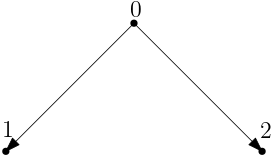
\includegraphics[width=40mm]{zero-horn.png}
\quad \quad  \scalebox{2.4}{$\hookrightarrow$} \quad  \quad 
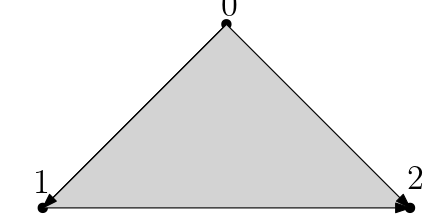
\includegraphics[width=45mm]{two-simplex.png}
 \caption{$\Lambda_0\left[2\right]$ (left) and $\Delta\left[2\right]$ (right)}
\end{figure}
\end{exmp}

\begin{defn}[Kan complex]
A simplical set $K_{\bullet}$ is a \textit{Kan complex} if every map $\Lambda_k\left[n\right] \to K$ can be extended to a map $\Delta\left[n\right] \to K$:
\[
\begin{tikzcd}
	{\Lambda_k\left[n\right]} & K \\
	{\Delta\left[n\right]}
	\arrow[hook, from=1-1, to=2-1]
	\arrow[from=1-1, to=1-2]
	\arrow[dashed, from=2-1, to=1-2]
\end{tikzcd}
.\]
\end{defn}

\begin{prop} $ $
\be
\item The set of maps $\left\{\Lambda_k\left[n\right] \subset \Delta\left[n\right]\right\}$ is a set of generating acyclic cofibrations, i.e., $K_{\bullet} \to L_{\bullet}$ is a fibration if and only if it has the RLP w.r.t. every inclusion  of the form $\Lambda_k\left[n\right] \subset \Delta\left[n\right]$.
\item The set of maps $\left\{\partial{\left[n\right]} \subset \Delta\left[n\right]\right\}$ is a set of generating cofibrations.
\ee
\end{prop}

\begin{corollary}
A simplicial set is fibrant if and only if it's a Kan complex.
\end{corollary}

\begin{exmp}\label{simpgrp}
Any simplicial group $G : \Delta^{\op} \to \mathsf{Grp}$ is a Kan complex when viewed as a simplicial set. (This is Prop.\ 8.2.8 of Weibel's \textit{Hom.\ Alg.}) For example, recall the inclusion $\Lambda_0\left[2\right] \subset \Delta\left[2\right]$ from \cref{zhorn}. Apply $G$ to this to get
\[
\begin{tikzcd}
	& {g_{0}} \\
	{g_1} && {g_2}
	\arrow[""{name=0, anchor=center, inner sep=0}, "{g_{01}}"', from=1-2, to=2-1]
	\arrow[""{name=1, anchor=center, inner sep=0}, "{g_{02}}", from=1-2, to=2-3]
	\arrow[dashed, from=2-1, to=2-3]
	\arrow["{?}"', shift left=2, Rightarrow, draw=none, from=0, to=1]
\end{tikzcd}
.\] We want to find a $2$-simplex $g \coloneqq g_{012} \in G_2$ along with a $1$-simplex $g_{12} \in G_1$ such that
\begin{align*}
d_2{g} & = g_{01}
\\ d_1{g} & = g_{02}
\\ d_0{g} & = g_{12}.
\end{align*}
It seems that taking
\[
g = \underbrace{\left(s_0{g_{02}}\right)\left(s_0^2g_0^{-1}\right)\left(s_0g_{01}\right)}_{s_0\left(g_{02}\left(s_0 g_0^{-1}\right)g_{01}\right)}, \ \quad G_0 \xrightarrow{s_0} G_1 \xrightarrow{s_0} G_2
\] doesn't work. But note that $g_{12} =  g_{02}g_{01}^{-1}$. Taking $g= s_0{g_{12}}$ may work.
\end{exmp}


\bigskip

\begin{defn}
Let $X$ be a space.
\be
\item We say that $X$ is \textit{weak Hausdorff} if the image in $X$ of a compact Hausdorff space is closed.
\item We say that $X$ is \textit{compactly generated} if a subspace $A \subset X$ is closed if and only if $A \cap K$ is closed in $K$ for every compact $K \subset X$.
\ee
\end{defn}

Let $\mathsf{WHCG}$ denote the full subcategory of $\mathsf{Top}$ on all weak Hausdorff compactly generated spaces. This is a  convenient category of spaces in the sense that it's cartesian closed:
\[
\Hom_{\mathsf{WHCG}}(X \times Y, Z) \cong \Hom_{\mathsf{WHCG}}(X, Z^Y)
.\]
Moreover, it contains all CW-complexes. 

\begin{theorem} $ $
\be
\item The adjunction
\[
\begin{tikzcd}
	{\mathsf{sSet}} & {\mathsf{WHCG}}
	\arrow[""{name=0, anchor=center, inner sep=0}, "{\left\lvert{-}\right\rvert}", curve={height=-12pt}, from=1-1, to=1-2]
	\arrow[""{name=1, anchor=center, inner sep=0}, "\sing", curve={height=-12pt}, from=1-2, to=1-1]
	\arrow["\dashv"{anchor=center, rotate=-90}, draw=none, from=0, to=1]
\end{tikzcd}
\] 
is a Quillen equivalence. 
\item There exists a Quillen equivalence 
$
\begin{tikzcd}
	{\mathsf{WHCG}} & {\mathsf{Top}}
	\arrow[shift left=1, from=1-1, to=1-2]
	\arrow[shift left=1, from=1-2, to=1-1]
\end{tikzcd}
.$
\ee
\end{theorem}


\section{Polynomial de Rham algebras}

\subsection{Lecture 27}

We turn to defining the polynomial deRham functor. This should be both an extension and a ``rationalization'' of the de Rham functor.
\begin{align*}
\mathsf{Man}^{\op} &  \to \dgca_{\R}^{\geq0}, \  M \mapsto \left(\Omega^{\bullet}(M), d\right)
\\ & \Downarrow
\\ \mathsf{Top}^{\op} & \to \dgca_{\Q}^{\geq 0},\ \text{or}
\\ \mathsf{sSet}^{\op} & \to \dgca_{\Q}^{\geq 0}
\end{align*}

Recall the cosimplicial space $\Delta^{\bullet}$ of all geometric $n$-simplices $\Delta^n \subset \R^{n+1}$. Moreover, $\Omega^{\bullet}$ is a contravariant functor to $\dgca_{\Q}^{\geq 0}$, with
\[
\Omega(n) = \frac{\Q\left[t_0, \ldots, t_n, d{t_0}, \ldots, d{t_n}\right]}{\left(\sum_{i=0}^n t_i = 1, \sum_{i=0}^n d{t_i}\right)}
.\] This is called the \textit{polynomial de Rham (dR) algebra} on $\Delta^n$. Indeed, we can make $\Omega(\Delta^{\bullet})$ a simplicial object $\Delta^{\op} \to \dgca_{\Q}^{\geq 0}$ in $\dgca_{\Q}^{\geq 0}$ as follows.

\medskip

Let $\Omega_n = \Omega(n)$. Let $u : \left[m\right] \to \left[n\right] $ be a morphism in $\Delta$. Define $\Omega(f) : \Omega(n) \to \Omega(m)$ by 
\[
t_i  \mapsto \sum_{j \in u^{-1}(i)}  t_j
.\] This means that $\sum_{i=0}^n{t_i} \mapsto \sum_{j=0}^m t_j$. The degeneracy $s_i$ and face $\partial_i$  maps are given, respectively, by
\begin{align*}
s_i{t_k} & = \begin{cases} t_{k+1} & i < k \\ t_k + t_{k+1} & i = k \\ t_k & i > k \end{cases}
\\ \partial_i{t_k} & = \begin{cases}
t_{k-1} & i < k
\\ 0 & i = k
\\ t_k & i > k
\end{cases}.
\end{align*} 
By construction, we have, for example, that
\begin{align*}
\partial_i(t_k t_e) & = \partial_i(t_k)\partial_i(t_e)
\\ \partial_i(d{t_k}) & = d(\partial_i{t_k})
.\end{align*} 
We conclude that $\Omega_{\bullet} \in \ob{s(\dgca_{\Q}^{\geq 0})}$.

\medskip

The \textit{polynomial (PL) de Rham functor} $\A : \mathsf{sSet}^{\op} \to \dgca_{\Q}^{\geq 0}$ is defined by
\begin{gather*}
K   \mapsto \Hom_{\mathsf{sSet}}(K, \Omega_{\bullet})  
\\ \left(\Hom_{\mathsf{sSet}}(K, \Omega_{\bullet})\right)^p  \equiv \Hom_{\mathsf{sSet}}(K, \Omega_{\bullet}^p)
\\ d{f}   \equiv d_{\Omega} \circ f, \ \ f : K \to \Omega_{\bullet}^p
\\ \left(f \cdot g\right)(x)   \equiv f(x) \cdot g(x), \ \ x \in K_n
.\end{gather*}
For any space $X$, the \textit{PL de Rham algebra} of $X$ is 
\[
 \Omega_{\PL}(X)  \equiv   \underbrace{\Hom_{\mathsf{sSet}}(\sing_{\bullet}(X), \Omega_{\bullet})}_{\A(\sing_{\bullet}(X))},
\]
i.e., the image of $X$ under the composite
\[
\mathsf{Top}^{\op} \xrightarrow{\sing_{\bullet}} \mathsf{sSet}^{\op} \xrightarrow{\A} \dgca_{\Q}^{\geq 0}.
\]
Note that 
\begin{align*}
\A(0) & = \A(\Delta\left[0\right]) 
\\ & = \Hom_{\mathsf{sSet}}(\Delta\left[0\right], \Omega)
\\ & \cong \Omega(\left[0\right]) \tag{\text{Yoneda}}
\\ & = \Omega(0)
\\ & = \Q.
\end{align*}
Now, define $\F: \dgca_{\Q}^{\geq 0} \to \mathsf{sSet}^{\op}$ by 
\begin{align*}
& B  \mapsto \Hom_{\dgca_{\Q}^{\geq 0}}(B, \Omega)
\\ &  \left(\Hom_{\dgca_{\Q}^{\geq 0}}(B, \Omega)\right)_n  \equiv  \Hom_{\dgca_{\Q}^{\geq 0}}(B, \Omega(n)).
\end{align*} We see that $\F(\Q) = 0 = \Delta\left[0\right]$ because for all $n \geq 0$, there is a unique map $\Q \to \Omega(n)$.



\subsection{Lecture 28}

Our big goal is to show that the pair $\left(\F, \A\right)$ of functors induces a Quillen equivalence on certain subcategories (which are related to nilpotence). To begin, we want to prove that it is a Quillen adjunction. This serves as our main adjunction for the course.

\begin{lemma}\label{mainadj}
The pair $\left(\F, \A\right)$ is an adjoint pair.
\end{lemma}
\begin{proof}
We must find a natural bijection
\begin{align*}
\Hom_{\mathsf{sSet}^{\op}}(\F(B), K) &  \cong \Hom_{\dgca_{\Q}^{\geq 0}}(B, \A(K)),\ \text{i.e.,}
\\ \Hom_{\mathsf{sSet}}(K, \F(B)) &  \cong \Hom_{\dgca_{\Q}^{\geq 0}}(B, \A(K)),\ \text{i.e.,}
\\ \Hom_{\mathsf{sSet}}(K, \Hom_{\dgca_{\Q}^{\geq 0}}(B, \Omega)) &  \cong \Hom_{\dgca_{\Q}^{\geq 0}}(B, \Hom_{\mathsf{sSet}}(K, \Omega)).
\end{align*}
For each $f: K \to \Hom_{\dgca_{\Q}^{\geq 0}}(B, \Omega)$, define $f^{\sharp} : B \to \Hom_{\mathsf{sSet}}(K, \Omega)$ by
\[
b \mapsto \left(x \mapsto f(x)(b)\right).
\] Conversely, for each $g : B \to \Hom_{\mathsf{sSet}}(K, \Omega)$, define $g^{\flat} : K \to \Hom_{\dgca_{\Q}^{\geq 0}}(B, \Omega)$ by
\[
x \mapsto \left(b \mapsto g(b)(x)\right)
.\] Then ${-}^{\sharp}$ and ${-}^{\flat}$ are inverses of each other. 
\end{proof} 

\begin{corollary}\label{overadj}
The adjunction $\F \dashv \A$ restricts to an adjunction $
\begin{tikzcd}
	{\dgca_{\Q}^{\geq 0}/\Q} & {\mathsf{sSet}_{\ast}^{\op}}
	\arrow[shift left=1, from=1-1, to=1-2]
	\arrow[shift left=1, from=1-2, to=1-1]
\end{tikzcd}
.$
\end{corollary}

For a sense of why \cref{overadj} is true, notice that $\F$ sends any map $B \to \Q$ to the pointed simplicial set $\underbrace{\F(\Q)}_{\ast} \to \F(B)$ and that $\A$ sends any pointed simplicial set $\ast \to K$ to the map $\A(K) \to \underbrace{\A(\ast)}_{\Q}$ over $\Q$.

\medskip

We now want to show that $\left(\F, \A\right)$ forms a Quillen adjunction. We must show that 
\bi
\item $\F$ sends cofibrations in $\dgca_{\Q}^{\geq 0}$ to cofibrations in $\mathsf{sSet}^{\op}$ (i.e., fibrations in $\mathsf{sSet}$) and
\item $\A$ sends fibrations in  $\mathsf{sSet}^{\op}$ (i.e., cofibrations in $\mathsf{sSet}$) to fibrations in $\dgca_{\Q}^{\geq 0}$.
\ei

\begin{lemma} \label{pres1}
The functor $\A$ sends cofibrations in $\mathsf{sSet}$ to fibrations in $\dgca_{\Q}^{\geq 0}$.
\end{lemma}
\begin{proof}
We must show that $\A$ sends any inclusion $K \hookrightarrow L$ to a degree-wise surjection $\A(L) \to \A(K)$. This map is surjective if and only if we can find lifts of the form
\[
\begin{tikzcd}
	K & {\Omega_{\bullet}^p} \\
	L & \ast
	\arrow[from=1-2, to=2-2]
	\arrow[from=2-1, to=2-2]
	\arrow[dashed, from=2-1, to=1-2]
	\arrow[hook, from=1-1, to=2-1]
	\arrow[from=1-1, to=1-2]
\end{tikzcd}
\] where $p \geq 0$. In this case, $K \hookrightarrow L$ has the LLP w.r.t each map of the form $\Omega^p \to \ast$. Thus, it suffices to show that $\Omega^p \to \ast$ is an acyclic fibration.
\bi
\item  By \cref{simpgrp}, $\Omega^p$ is a Kan complex as a simplicial (abelian) group.
\item Note that  $\Omega^p \to \ast$ is a map of fibrant, cofibrant objects. By \cref{qWhite}, this map is a weak equivalence if and only if it's a homotopy equivalence. Thus, it suffices to show that $\Omega^p \to \ast$ is a homotopy equivalence with homotopy inverse $0 \hookrightarrow \Omega^p$. We want a left homotopy 
\[
\Omega^p \times \Delta\left[1\right] \to \Omega^p
\] between $\Omega^p \xrightarrow{\id} \Omega^p$ and $\Omega^p \to 0 \to \Omega^p$ (the constant map at $0$). Note that
\[
\left(\Omega^p \times \Delta\left[1\right]\right)_n = \Omega(n)^p \times \Delta\left[1\right]_n = \bigoplus_{\alpha \in \Delta\left[1\right]_n}\Omega(n)^p
.\] We shall define the left homotopy after discussing homotopies in $\mathsf{sSet}$.
\ei
\end{proof}

\subsection{Lecture 29}

Our current plan has three parts.
\be
\item Finishing the main theorem: $\left(\F, \A\right)$ induces a Quillen equivalence on suitable subcategories
\item Quillen (minimal) models of $\mathsf{sSet}$ and $\dgca_{\Q}^{\geq 0}$ in the $L_{\infty}$-world
\item Application to Mysterious Duality in string theory
\ee

To finish our main theorem, we must look at the notion of homotopy in $\mathsf{sSet}$.

\smallskip

\begin{theorem}[Fundamental adjunction]
The pair $\left(\F, \A\right)$ is a Quillen adjunction
\[
\begin{tikzcd}
	{\dgca_{\Q}^{\geq 0}} & {\mathsf{sSet}^{\op}}
	\arrow[shift left=1, from=1-1, to=1-2]
	\arrow[shift left=1, from=1-2, to=1-1]
\end{tikzcd} 
.\]
\end{theorem}
\begin{proof}
First, we know that this is an adjunction by \cref{mainadj}. Second, up to our discussion of homotopy in $\mathsf{sSet}$, we know that $\A$ sends fibrations in $\mathsf{sSet}^{\op}$ to fibrations in $\dgca_{\Q}^{\geq 0}$ by \cref{pres1}. Finally, we must show that $\F$ sends cofibrations in $\dgca_{\Q}^{\geq 0}$ to cofibrations in $\mathsf{sSet}^{\op}$, i.e., fibrations in $\mathsf{sSet}$.

\medskip

With this in mind, we want to show that the maps
\[
\begin{tikzcd}
	{\Omega^p} & {\Omega^p}
	\arrow["\id", shift left=1, from=1-1, to=1-2]
	\arrow["0"', shift right=1, from=1-1, to=1-2]
\end{tikzcd}
\] are left homotopic. A \textit{left homotopy} for simplicial sets or for simplicial $\Q$-vector spaces is a left homotopy with respect to the cylinder object
\[
\begin{tikzcd}[column sep = large]
	{K \coprod K} & {} & {K \times \Delta\left[1\right]} & {\left\lvert{K}\right\rvert \times \left\lvert{\Delta\left[1\right]}\right\rvert} \\
	& {} && {} \\
	& {} & {K\times \ast} & {\left\lvert{K}\right\rvert}
	\arrow["{\id \times \Delta\left[\delta^1\right]\ +\ \id \times \Delta\left[\delta^0\right]}", hook, from=1-1, to=1-3]
	\arrow[""{name=0, anchor=center, inner sep=0}, "\wr", from=1-3, to=3-3]
	\arrow["\nabla"', from=1-1, to=3-3]
	\arrow["\wr", from=1-4, to=3-4]
	\arrow[shorten <=18pt, shorten >=18pt, Rightarrow, from=2-4, to=0]
\end{tikzcd}, \ \quad \left\lvert{\Delta\left[1\right]}\right\rvert  = \Delta^1 \sim \ast
,\] in the sense of \cref{lhom}. In general, a left homotopy $K \times \Delta\left[1\right] \to L$ is equivalent to a map \linebreak $K \to \underline{\Hom}_{\mathsf{sSet}}(\Delta\left[1\right], L)$ thanks to the natural isomorphism
\[
\Hom_{\mathsf{sSet}}(K \times X,L) \cong \Hom_{\mathsf{sSet}}(K, \underline{\Hom}_{\mathsf{sSet}}(X,L)), \ \quad  \underline{\Hom}_{\mathsf{sSet}}(X,L)_n \equiv \Hom_{\mathsf{sSet}}(\Delta\left[n\right] \times X, L)
.\] This definition of the internal hom as a simplicial set is motivated by the equations
\[
\Hom_{\mathsf{sSet}}(\Delta\left[n\right] \times X, L) = \Hom_{\mathsf{sSet}}(\Delta\left[n\right] , \underline{\Hom}_{\mathsf{sSet}}(X,L)) = \underline{\Hom}_{\mathsf{sSet}}(X,L)_n 
.\] In particular, note that 
\begin{align*}
\underline{\Hom}_{\mathsf{sSet}}(\Delta\left[1\right], L)_n  = &  \Hom_{\mathsf{sSet}}(\Delta\left[n\right] \times \Delta\left[1\right], L)
\\ &\quad  \updownarrow  \tag{EZ-AW}
\\ & \Hom_{\mathsf{sSet}}(\Delta\left[n+1\right], L) 
\\ & \quad  \parallel
\\ & \ \  L_{n+1}.
\end{align*}
This means that a \textit{simplicial} homotopy $K \times \Delta\left[1\right] \to L$ is the same as a collection of maps $K_n \to L_{n+1}$. In particular, a homotopy $\id_{\Omega^p(n)} \overset{\ell}{\sim} 0$ amounts to a formula of the form $\Omega^p(n) \to \Omega^p(n+1)$ for each $p\geq 0$:
\begin{align*}
1 & \mapsto T^2
\\ t_i & \mapsto T\cdot t_{i+1}
\\ d{t_i} & \mapsto T\cdot d{t_{i+1}} - d{T}\cdot t_{i+1}, \ \quad T \equiv t_1 + \cdots + t_n
.\end{align*}

\medskip

Next, we want to show that $\F$ sends cofibrations in $\dgca_{\Q}^{\geq 0}$ to fibrations in $\mathsf{sSet}$. Suppose that $i : B \to C$ is such a cofibration. To see that $\F_i$ is a fibration, it suffices to check the RLP of $\F_i$ with respect to all generating acyclic cofibrations,

\[
\begin{tikzcd}
	{\Lambda\left[n\right]_k } & {\Delta\left[n\right]} & {n,k \geq 0}
	\arrow["\sim", hook, from=1-1, to=1-2]
\end{tikzcd}
.\]

Our adjunction $\F \dashv \A$ gives us an equivalence

\[
\begin{tikzcd}
	{\Lambda\left[n\right]_k} & {\F{C}} \\
	{\Delta\left[n\right]} & {\F{B}}
	\arrow[from=2-1, to=2-2]
	\arrow["\wr"', hook', from=1-1, to=2-1]
	\arrow[from=1-1, to=1-2]
	\arrow["{\F_i}", from=1-2, to=2-2]
	\arrow[dashed, from=2-1, to=1-2]
\end{tikzcd}
\quad \iff \quad 
\begin{tikzcd}
	B & {\A(\Delta\left[n\right])} \\
	C & {\A(\Lambda\left[n\right]_k)}
	\arrow[from=2-1, to=2-2]
	\arrow["i"', hook', from=1-1, to=2-1]
	\arrow[from=1-1, to=1-2]
	\arrow[two heads, from=1-2, to=2-2]
	\arrow[dashed, from=2-1, to=1-2]
\end{tikzcd}.
\]
Thus, it suffices to show that the map $\A(\Delta\left[n\right]) \to \A(\Lambda\left[n\right]_k)$ is an acyclic fibration, i.e., that the induced map
\[
\underbrace{H^{\bullet}(\A(\Delta\left[n\right]))}_{\Q} \xrightarrow{\overset{?}{\sim}} H^{\bullet}(\A(\Lambda\left[n\right]_k))
\] is an isomorphism.

\medskip

For any simplicial set $K$, define the \textit{simplicial cochain complex of $K$} $C^{\bullet}(K)$ by
\begin{align*}
C^n(K) &  =\Hom(K_n, \Q)
\\ d{f}(x) & = \sum_{i=0}^{n+1} \left({-1}\right)^if(d_i{x}), \ \quad x \in K_{n+1}
.\end{align*}

\begin{prop}\label{isoreal}
$H^{\bullet}(C^{\bullet}(K)) = H^{\bullet}(\left\lvert{K}\right\rvert)$.
\end{prop}

Next, define $\rho : \A(K) \to C^{\bullet}(K)$ by integration of PL differential forms over geometric simplices:
\[
\A(K)^p \ni  \omega \  \mapsto  \ \left(K_p \ni x \ \mapsto \ \int_{\Delta^p}\omega(x)\right)
,\] where $\omega(x) \in \Omega(p)^p$.  

\subsection{Lecture 30}

\begin{theorem}[Simplicial de Rham]\label{SDR}
The cochain map $\rho$ is a quasi-isomorphism of $\Q$-complexes, i.e., induces an isomorphism 
\[
H^{\bullet}(\A(K)) \xrightarrow{\sim} H^{\bullet}(C^{\bullet}(K))
\] of graded-$\Q$-vector spaces. 
\end{theorem}
\begin{proof}[Proof sketch] $ $
\be
\item \textbf{Poincar\'e lemma:} 
\begin{align*}
H^{\bullet}(\A(\Delta\left[n\right])) &  \cong \Q 
\\ & \cong H^{\bullet}(\Delta^n, \Q) 
\\ & \cong H^{\bullet}(C^{\bullet}(\Delta\left[n\right])). \tag{\cref{isoreal}} 
\end{align*}
\item \textbf{Mayer-Vietoris sequence:} 

For any pushout square
\[
\begin{tikzcd}
	K & M \\
	L & N
	\arrow["i"', hook', from=1-1, to=2-1]
	\arrow["h"', from=2-1, to=2-2]
	\arrow["g", from=1-2, to=2-2]
	\arrow["j", from=1-1, to=1-2]
	\arrow["\lrcorner"{anchor=center, pos=0.125, rotate=180}, draw=none, from=2-2, to=1-1]
\end{tikzcd}
\] in $\mathsf{sSet}$,  we have a short exact sequence
\[
0 \longrightarrow \A(N) \xrightarrow{\left(\A(h), {-\A(g)}\right)} \A(L) \oplus \A(M) \xrightarrow{\A(i) + \A(j)} \A(K) \longrightarrow 0 
\] of $\Q$-vector spaces. This has a LES in cohomology, known as the M-V sequence for $H^{\bullet}(\A(N))$.

Likewise, we have a short exact sequence
\[
\begin{tikzcd}
	0 & {C^{\bullet}(N)} & {C^{\bullet}(L)\oplus C^{\bullet}(M)} & {C^{\bullet}(K)} & 0
	\arrow[from=1-1, to=1-2]
	\arrow[from=1-4, to=1-5]
	\arrow[from=1-2, to=1-3]
	\arrow[from=1-3, to=1-4]
\end{tikzcd}
\] along with the M-V sequence for $H^{\bullet}(C^{\bullet}(K))$. 

We see that $\rho$ induces a morphism between the two SES's. The five lemma thus implies that if $\rho$ induces an isomorphism on cohomology for $L$, $M$, and $K$, then it also induces one for $N$.
\item Every simplicial set is the pushout along a map of the form $\coprod_{\alpha} \partial{\Delta\left[n\right]} \hookrightarrow \coprod_{\alpha}\Delta\left[n\right]$.
\ee
\end{proof}

\begin{remark}
In fact, $\rho$ induces an isomorphism of cohomology \emph{rings} as it can be represented as a zig-zag of quasi-isomorphism of DGA's.
\[
\begin{tikzcd}
	& \bullet && \bullet \\
	{\A(K)} && \cdots && {C^{\bullet}(K)}
	\arrow["{\textit{q-iso}}", from=1-2, to=2-1]
	\arrow["{\textit{q-iso}}", from=1-2, to=2-3]
	\arrow["{\textit{q-iso}}", from=1-4, to=2-3]
	\arrow["{\textit{q-iso}}", from=1-4, to=2-5]
	\arrow["\rho"', curve={height=18pt}, from=2-1, to=2-5]
\end{tikzcd} \ \quad \ \implies \ \quad \ \text{$H^{\bullet}(\rho)$ is an iso.}
\]
\end{remark}

\medskip

Now, both $H^{\bullet}(C^{\bullet}(\Delta\left[n\right]))$ and  $H^{\bullet}(C^{\bullet}(\Lambda\left[n\right]_k))$  are isomorphic to $\Q$ thanks to \cref{isoreal}. Thus, by \cref{SDR}, we have that $H^{\bullet}(\A(\Delta\left[n\right])) \cong \Q \cong H^{\bullet}(\A(\Lambda\left[n\right]_k))$.

\end{proof}

\medskip

Let's turn to the homotopy theory of our fundamental adjunction. We have an adjunction
\[
\begin{tikzcd}
	{\ho(\dgca_{\Q}^{\geq 0})} & {\ho(\mathsf{sSet}^{\op})}
	\arrow[""{name=0, anchor=center, inner sep=0}, "{\R{\A}}", curve={height=-12pt}, from=1-2, to=1-1]
	\arrow[""{name=1, anchor=center, inner sep=0}, "{\Ll{\F}}", curve={height=-12pt}, from=1-1, to=1-2]
	\arrow["\dashv"{anchor=center, rotate=-90}, draw=none, from=1, to=0]
\end{tikzcd}
.\] Every object of $\mathsf{sSet}$ is cofibrant, and any cofibrant replacement of a cofibrant object $K$ (such as $K$ itself) is unique up to homotopy in a certain sense.  Therefore, $\R{\A} = \A(R{K}) = \A(K)$ because $R{K}$ is a cofibrant replacement of $K$ in $\mathsf{sSet}$. Moreover, $\Ll{\F}(B) = \F(Q{B})$, which is automatically a Kan complex.

\begin{defn} $ $
\be
\item Let $K$ be a simplicial set. A \textit{Sullivan  minimal model} of $K$ is a minimal Sullivan model of $\A(K)$, i.e., a minimal Sullivan algebra $\M(K)$ together with a quasi-isomorphism $\M(K) \to \A(K)$.
\item Let $X$ be a topological space. A \textit{Sullivan model} of $X$ is a Sullivan minimal model of $ \sing_{\bullet}(X)$.
\ee
\end{defn}

\Cref{SAcf} implies that $\M(K)$ is a cofibrant replacement of $\A(K)$.

\medskip

We can make $\M$ a functor so that we have a diagram
\[
\begin{tikzcd}
	{\ho(\underbrace{\mathsf{SMA}}_{\substack{\text{homolog.} \\ \text{conn.} \\ \text{Sull. min.} \\ \text{algebras}}})} & {\ho(\underbrace{\mathsf{sSet}_0^{\op}}_{\text{conn. ssets}})}
	\arrow["\F", shift left=1, from=1-1, to=1-2]
	\arrow["\M", shift left=1, from=1-2, to=1-1]
\end{tikzcd}
.\] This is actually an adjunction.

\bigskip

\textbf{Homotopy groups:}

\medskip

Recall that for any $B \in \ob(\dgca_{\Q}^{\geq 0}/\Q)$, we have
$
\pi^n(B) = H^n(I{B})
$
 by definition, where $I{B} = \faktor{m_B}{m_B^2}$ and $m = \ker(B \to \Q)$. 

\medskip


Let $K$ be a pointed simplicial set, i.e., an object of $\mathsf{sSet}_{\ast}$. (Its distinguished point is precisely a map $\Delta\left[0\right] \to K$.) Assume that $K$ is a Kan complex. Define the homotopy groups of $K$ as follows. Let $\pi_0(K)$ be the coequalizer

\[
\begin{tikzcd}
	{X_1} & {X_0} & {\faktor{X_0}{X_1}}
	\arrow["{d_0}", shift left=1, from=1-1, to=1-2]
	\arrow["{d_1}"', shift right=1, from=1-1, to=1-2]
	\arrow[two heads, from=1-2, to=1-3]
\end{tikzcd}.
\]
This is precisely the set $\left[\Delta\left[0\right], K\right]$ of homotopy classes of maps. Further, for any $n \geq 1$, let \linebreak $\pi_n(K) = \left[\left(\Delta\left[n\right], \partial{\Delta\left[n\right]}\right), \left(K, \ast\right)\right]$. Note that

\begin{align*}
\pi_n(K) & = \left[\left(\partial{\Delta\left[n+1\right]}, v_0\right), \left(K, \ast\right)\right]
\\ & = \left[\left(S^n, N\right), \left(\left\lvert{K}\right\rvert, \ast\right)\right]
\\ & = \pi_n(\left\lvert{K}\right\rvert, \ast)
.\end{align*}

Thus, we have at least four ways of defining the homotopy group. The rational homotopy groups of $K$ are defined as

\[
\pi_n^{\Q}(K) = 
\begin{cases}
\pi_n(K) \otimes_{\Z} \Q & n \geq 2
\\ \frac{\pi_1(K)}{\left[\pi_1(K), \pi_1(K)\right]} \otimes_{\Z} \Q & n =1
\end{cases}
.\]

\subsection{Lecture 31}

We want to study the homotopy groups of  a cofibrant augmented DGCA $B \to \Q$ and of the simplicial set $\F{B}$. Let $K$ be a pointed Kan complex. To endow  $\pi_n(K)$ with a group structure for all $n\geq 1$, let $\left[f\right],\left[g\right] \in  \left[\left(\Delta\left[n\right], \partial{\Delta\left[n\right]}\right), \left(K, \ast\right)\right]$. Define $\varphi : \Lambda_n\left[n+1\right] \to K$ by 

\[
\varphi(i) = \begin{cases}
s_0s_0\cdots s_0(\ast) & 0 \leq i \leq n-2
\\ g & i = n-1
\\ f & i = n+1
\end{cases}
.\]

As $K$ is a Kan complex, this horn may be filled to a map $\tilde{\varphi} : \Delta\left[n+1\right] \to K$. By the simplicial identities, we have that

\[
d_id_n{\tilde{\varphi}} = d_{n-1}d_i{\tilde{\varphi}} = s_0s_0\cdots s_0(\ast)
.\] 

Let  $\left[f\right]\cdot\left[g\right] = \left[d_n{\tilde{\varphi}}\right]$.

\[
\begin{tikzcd}
	& 0 \\
	1 && 2
	\arrow["f"', from=1-2, to=2-1]
	\arrow["g"', from=2-1, to=2-3]
	\arrow["{f\cdot g}", dashed, from=1-2, to=2-3]
\end{tikzcd}
\]

This is a group operation. In fact, $\pi_n(\F{B})$ is naturally a $\Q$-vector space and thus isomorphic to $\pi_n^{\Q}(\F{B})$.

\begin{theorem}\label{dualiso}
Let $B$ be a cofibrant augmented DGCA$^{\geq 0}$. 
\be[label = (\arabic*)]
\item If $B$ is homologically connected (i.e., $H^0(B) \cong \Q$), then $\pi_0(\F{B}) = \ast$. 
\item If $n \geq 1$, then there exists a natural bijection
\[
\pi_n(\F{B}) \xrightarrow{\sim} \Hom_{\Q}(\pi^n{B}, \Q)
\] of sets.
\item if $n \geq 2$, then this bijection is a group isomorphism. 
\item If $n =1$, then it is a group isomorphism as long as 
\[
x\in B^1 \implies d{x} \in \Q\left[B^0, d{B^0}\right] \subset B
.\]
\ee
\end{theorem}
\begin{proof}[Proof sketch] 
First,  suppose that $H^0(B) \cong \Q$. By \cref{minmod}, we have a minimal Sullivan algebra $\M(B)$ and a weak equivalence $\M(B) \xrightarrow{\sim} B$. Since both $B$ and $\M(B)$ are cofibrant, our proof of \cref{KB} shows that the induced map $\F{\M(B)} \to \F{B}$ is a weak equivalence. Hence $\left\lvert{\F{B}}\right\rvert \simeq \left\lvert{\F{\M(B)}}\right\rvert$, and  we have that 
\begin{align*}
\pi_0(\F{B}) & = \pi_0(\F{\M(B)}) 
\\ & = \left[\Delta\left[0\right], \F{\M(B)}\right]
\\ & =   \left[\F{\M(B)}, \Delta\left[0\right]\right]^{\op}
\\ & =  [\M(B), \underbrace{\A(\Delta\left[0\right])}_{\emptyset}] \tag{$\Ll{\F} \dashv \R{\A}$}
\\ & = \left[\M(B), \Q\right] 
\\ & = \ast. \tag{$\M(B) = S(V), \ V = \bigoplus_{\geq 1}V^n$}
\end{align*}
This proves (1).

Next, suppose that $n > 1$. By \cref{cof-fib}, we have that

\[
\pi_n(\F{B})  = \left[\partial{\Delta\left[n+1\right]}, \F{B}\right] \cong \left[B, \A(\partial{\Delta\left[n+1\right]})\right]
.\]

Let 
\[
V(n) = \faktor{\Q\left[x_n\right]}{\left(x_n^2\right)}, \ \quad \left\lvert{x_n}\right\rvert \equiv n
.\] This has homology $H^{\bullet}(S^n; \Q)$. Further, \cref{SDR} gives us a weak equivalence  \linebreak $ \A(\partial{\Delta\left[n+1\right]}) \xrightarrow{\sim} C^{\bullet}(\partial{\Delta\left[n+1\right]})$, and $C^{\bullet}(\partial{\Delta\left[n+1\right]})$ also has homology  $H^{\bullet}(S^n; \Q)$. Indeed, the map $V(n) \xrightarrow{\sim}  \A(\partial{\Delta\left[n+1\right]})$ defined by

\[
x_n \ \ \mapsto \ \ \text{a closed PL form representing a generator of $H^n(S^n;\Q) \cong \Q$}
\] is a weak equivalence. This means that $ \left[B, \A(\partial{\Delta\left[n+1\right]})\right] \cong  \left[B, V(n)\right]$.

\begin{prop}
$\left[B, V(n)\right] \cong \Hom_{\Q}(\pi^n(B), \Q)$.
\end{prop}

This sequence of bijections respects the group structure of $\pi_n$. Wlog, replace $B$ with $\M(B)$. We have a cofibration $S(V(n-1)) \hookrightarrow S(V(n))$. By taking the pushout of this along $S(V(n-1)) \to \Q$,  we can show that $\left(S(V(n)/V(n-1)), d \equiv 0\right)$ has the same $\pi^n$ as $B$.  This also has a coalgebra structure: $B \to B \otimes B$, which induces a monoid structure on $\F{B}$. By the Eckmann-Hilton argument, the set
\[
\underbrace{\left[B, \A(\partial{\Delta\left[n+1\right]})\right]}_{\left[\partial{\Delta\left[n+1\right]}, \F{B}\right]}
\] is a monoid with the same structure as that on $\pi_n(\F{B})$. Moreover, the coalgebra structure defines a monoid structure on $\pi^n(B)^{\vee}$ identifiable as $+$.

\end{proof}

\subsection{Lecture 32}

Let $X$ be a rational space. Suppose that $\F{\M{(\A{X})}} \overset{\textit{w.e.}}{\sim} X$. Then

\begin{align*}
\pi_n(X) &  \cong \pi_n(\Ll{\F{\A{X}}}) \tag{$\M$ cofibrant replacement}
\\  & \cong \pi^n(\M(\A{X}))^{\vee}   \tag{\cref{dualiso}}.
\end{align*}

In particular, for all $n \geq 1$, we have that $\pi_n(S^n) \cong \pi^n(\M(S^n))^{\vee}$. As in the real de Rham case, we can guess a minimal Sullivan model of $\A(\partial{\Delta\left[n+1\right]})$:
\[
\M(S^n) = \begin{cases}
\Q\left[x_n\right] & n \text{ odd}
\\ \Q\left[x_n, y_{2n-1} \mid d{y_{2n-1}} = x_n^2\right] & n \text{ even}
\end{cases},
\] where $\left\lvert{x_n}\right\rvert = n$. Note that $\pi^k(\M(S^n)) = \left(I{\M(S^n)}\right)^k$. Specifically, $I{\Q\left[x_n\right]} = \Q{x_n}$ when $n$ is odd, in which case
\[
\pi_k^{\Q}(S^n) = \begin{cases}
\Q & k = n
\\ 0 & k \ne n
\end{cases}
\] for all $k \geq 1$. And when $n$ is even, we have that 
\begin{align*}
I{ \Q\left[x_n, y_{2n-1} \mid d{y_{2n-1}} = x_n^2\right] } & = \Q{x_n} \oplus \Q{y_{2n-1}}
\\ & \Downarrow
\\ \pi_k^{\Q}(S^n) & = \begin{cases}
\Q & k = n, 2n-1
\\ 0 &  \text{otherwise}
\end{cases}.
\end{align*}

By contrast, in the non-Sullivan case, we have that $H^{\bullet}(S^n; \Q) \cong \faktor{\Q\left[x_n\right]}{\left(x_n^2\right)}$.

\medskip

A \textit{rationalization} of a space $X$ is a space $X_{\Q}$ together with a map $X_{\Q} \to X$ inducing an isomorphism
\[
\pi_k(X_{\Q}) \cong \pi_k(X) \otimes_{\Z} \Q.
\] Thus, every space of the form $\F{B}$ is a rationalization of itself. 

\textbf{Main theorem of RHT:}

\medskip

The Quillen adjunction  $\F \dashv  \A$
\[
\begin{tikzcd}
	{\dgca_{\Q}^{\geq 0}} & {\mathsf{sSet}_{\ast}^{\op}}
	\arrow[shift left=1, from=1-1, to=1-2]
	\arrow[shift left=1, from=1-2, to=1-1]
\end{tikzcd} 
\]
induces an equivalence of categories

\[  
\ho(\dgca_{\Q}^{\geq 0, \ft}) \xrightarrow{\sim} \ho(\Q{\nil}_{\ast}^{\ft})^{\op}
.\]

Here, $\dgca_{\Q}^{\geq 0, \ft}$ denotes the full subcategory of cohomologically connected DGCA's of \textit{finite type}, i.e., \linebreak $\dim_{\Q}B^n < \infty$ for all $n \geq 0$ (equivalently, $\dim_{\Q}\pi^n(B) < \infty$). Further, $\Q{\nil}_{\ast}^{\ft}$ denotes the category of cohomologically connected spaces $X$ that are

\bi
\item rational as simplicial sets, i.e., have rational homotopy groups,
\item of finite type, i.e., $\dim_{\Q}H^n(X;\Q) < \infty$ for all $n \geq 0$, and
\item nilpotent, i.e., $\pi_1(X)$ is nilpotent and acts nilpotently on $\pi_k(X)$ (via the universal cover of $X$) for all $k \geq 2$.
\ei

A group $G$ is \textit{nilpotent} if the sequence
\begin{align*}
G_0 &  \equiv G
\\ G_{n+1} & \equiv \left[G, G_n\right] 
\end{align*}
of groups becomes trivial for some $n$. Further, for any groups $G$ and $A$ with $G$ acting on $A$, we say that $G$ \textit{acts nilpotently} on $A$  if the sequence 
\begin{align*}
A_0 & \equiv A
\\ A_{n+1} & \equiv  \left\langle{ga - a \mid g \in G, a \in A_n}\right\rangle
\end{align*}
of groups becomes trivial for some $n$.


\begin{exmp} $ $
\be
\item $S^1$ is nilpotent.
\item Any simply connected space is nilpotent.
\item $\RP^2$ is not nilpotent.
\item $S^1 \vee S^1$ is not nilpotent.
\ee
\end{exmp}

\subsection{Lecture 33}

Recall the main theorem of RHT. The pair $\left(\F, \A\right)$ is a Quillen adjunction, which is actually a Quillen equivalence for

\[
\begin{tikzcd}
	{\dgca_{\Q}^{\geq 0, \ft, \text{h-conn.}}} & {\left(\mathsf{sSet}_{\Q}^{\ft, \nilp}\right)^{\op}}
	\arrow[shift left=1, from=1-1, to=1-2]
	\arrow[shift left=1, from=1-2, to=1-1]
\end{tikzcd}
\]

For spaces, we may combine this equivalence with the Quillen equivalence

\[
\begin{tikzcd}[column sep=large]
	{\left(\mathsf{sSet}_{\Q}^{\ft, \nilp}\right)^{\op}} & {\left(\mathsf{WHCG}_{\Q}^{\ft, \nilp}\right)^{\op}}
	\arrow["{\left\lvert{-}\right\rvert}", shift left=1, from=1-1, to=1-2]
	\arrow["{\sing_{\bullet}}", shift left=1, from=1-2, to=1-1]
\end{tikzcd}
\]

induced by the equivalence between $\mathsf{sSet}^{\op}$ and $\mathsf{WHCG}^{\op}$.

\medskip

The rationalization of a space (in the sense of \cref{ratz}) always exists.

\begin{lemma}
The counit $K \mapsto \F{\A{K}}$ of $\F \dashv \A$ is a rationalization.
\end{lemma}

Recall that if $\left(\F : \c \to \d,\ \A : \d \to \c \right)$ is any adjoint pair, then its \textit{unit} is the natural transformation \linebreak $\left\{B \xrightarrow{u_B} \A{\F(B)}\right\}_{B \in \ob{\c}}$ given by

\begin{align*}
\Hom_{\c}(B, \A{\F(B)}) &  \cong \Hom_{\d}(\F(B), \F(B))
\\ u_B \ \ & \leftmapsto \ \ \id_{\F(B)}.
\end{align*}

Likewise, the \textit{counit} is the natural transformation $\left\{\F{\A(K)} \xrightarrow{c_K} K \right\}_{K \in \ob{\d}}$ given by

\begin{align*}
\Hom_{\d}(\F{\A(K)}, K) &  \cong \Hom_{\c}(\A(K), \A(K))
\\ c_K \ \ & \leftmapsto \ \ \id_{\A(K)}.
\end{align*}

In our case, the adjunction counit is an isomorphism $\F{\A} \to \id_{\mathsf{sSet}^{\op}}$ on $\mathsf{sSet}^{\op}$, i.e., an isomorphism $ \id_{\mathsf{sSet}} \to \F{\A} $ on $\mathsf{sSet}$.

\medskip

Recall that $\pi_n(\F(B)) \cong \Hom_{\Q}(\pi^n(B), \Q)$ for all $n \geq 1$. Hence $H_n(\F(B); \Z)$ is a $\Q$-vector space. It follows that the rational homotopy type of a nilpotent, finite-type space $X$ is determined by the (quasi-)isomorphism class of its Sullivan minimal model. 

\medskip

Next, we'll study Quillen models via $L_{\infty}$-algebras as well as dg-Lie algebras.

\section{Quillen models}

\subsection{Lecture 34}

\begin{defn}[DGLA]
A \textit{dg-Lie algebra} is a chain complex $\left(L_{\bullet} \coloneqq \bigoplus_{n \in \Z} L_n, d : L_n \to L_{n-1}\right)$, $d^2 =0$, equipped with a \textit{graded-Lie bracket} $\left[{-}, {-}\right] : L_{\bullet} \otimes L_{\bullet} \to L_{\bullet}$, $L_p \otimes L_q \to L_{p+q}$, such that
\be[label=(\arabic*)]
\item (\textit{graded-skew}) $\left[x,y\right] = {-\left({-1}\right)^{\left\lvert{x}\right\rvert \left\lvert{y}\right\rvert}\left[y,x\right]}$.
\item (\textit{graded-Jacobi}) $\left({-1}\right)^{\left\lvert{x}\right\rvert \left\lvert{z}\right\rvert}\left[x, \left[y, z\right]\right] +
\left({-1}\right)^{\left\lvert{y}\right\rvert \left\lvert{x}\right\rvert}\left[y, \left[z, x\right]\right] + 
\left({-1}\right)^{\left\lvert{z}\right\rvert \left\lvert{y}\right\rvert}\left[z, \left[x, y\right]\right]
= 0$.
\item (\textit{graded-Leibniz (derivation)}) $d{\left[x,y\right]} = \left[d{x},y\right] + \left({-1}\right)^{\left\lvert{x}\right\rvert}\left[x,d{y}\right]$.
\ee
\end{defn}

We say that $L$ is \textit{connected} if $L = L_{>0}$. 

\begin{exmp} The following are dg-Lie algebras.
\be
\item Any Lie algebra $L$, with $L = L_0$ and $d =0$.
\item Any chain complex $\left(V_{\bullet}, d\right)$, with $\left[{-}, {-}\right] \equiv 0$. This is called an \textit{abelian} dg-Lie algebra.
\item Any dg-associative algebra $\left( A_{\bullet} = \bigoplus_{n \in \Z} A_n, d\right)$, with $\left[a,b\right] \equiv ab - \left({-1}\right)^{\left\lvert{a}\right\rvert \left\lvert{b}\right\rvert}ba$.

This defines a functor $\left({-}\right)^{\mathsf{Lie}} : \mathsf{dga} \to \mathsf{dgla}$,  which is right adjoint to the \textit{universal enveloping algebra} $\U : \mathsf{dgla} \to \mathsf{dga}$.
\begin{align*}
\U{L} &  \equiv \faktor{T(L)}{I}
\\ T(L) & \equiv \bigoplus_{n \geq 0}L^{\otimes n}, \ \ I  \equiv  \left(x \otimes y - \left({-1}\right)^{\left\lvert{x}\right\rvert \left\lvert{y}\right\rvert} y \otimes x - \left[x,y\right] \mid x, y \in L\right)
\\ \left(x_1 \otimes \cdots \otimes x_p\right) \left(y_1 \otimes \cdots \otimes y_q\right) & \equiv x_1 \otimes \cdots \otimes x_p \otimes y_1 \otimes \cdots \otimes y_q,\   \text{$d$ extented as derivation from $L$ to $T(L)$}
\end{align*}
\ee
\end{exmp}

\begin{note} $ $
\be
\item There is a natural isomorphism $\U( L \oplus M) \cong \U(L) \otimes \U(M)$. 
\item If $L$ is an abelian DGLA, then $\U{L} = S(L)$. In particular,  $\U(0) = k$.
\item The algebra $\U{L}$ is a dg-Hopf algebra. This means that it has extra structure coming from 
\bi
\item $L \xrightarrow{x \mapsto \left(x,x\right)}  L \oplus L \ \  \implies \ \ \underbrace{\U{L} \xrightarrow{\Delta} \U{L} \otimes \U{L}}_{\textit{comultiplication}}$, 
\item $L \to 0  \ \  \implies \ \ \underbrace{\U{L} \to k}_{\textit{counit}}$, and
\item  $\underbrace{s : L \xrightarrow{x \mapsto {-x}} L}_{\textit{antihomomorphism}}   \ \  \implies \ \    \underbrace{S : \U{L} \to \U{L}}_{\textit{antipode}} $.

Note that 

\[
S(a\cdot b) =  \left({-1}\right)^{\left\lvert{a}\right\rvert \left\lvert{b}\right\rvert} (S{b}\cdot S{a})
.\]

Also, note that 
\begin{align*}
\left[x,y\right] \overset{s}{\longmapsto} {-\left[x,y\right]} & = \left({-1}\right)^{\left\lvert{x}\right\rvert\left\lvert{y}\right\rvert}\left[y,x\right] 
\\ & =  \left({-1}\right)^{\left\lvert{x}\right\rvert\left\lvert{y}\right\rvert}\left[{-y},{-x}\right] 
\\ & \ne {- \left({-1}\right)^{\left\lvert{x}\right\rvert\left\lvert{y}\right\rvert}\left[y,x\right]}
\\ & = \left[x,y\right]
\\ & = \left[{-x}, {-y}\right].
\end{align*}
Hence $s\left[x, y\right] = \left({-1}\right)^{\left\lvert{x}\right\rvert \left\lvert{y}\right\rvert} \left[s{y}, s{x}\right]$.
\ei

This structure makes $\U{L}$ a dg-associative algebra with a compatible dg-coassociative  counital coalgebra. It's coassociative as
\[
\begin{tikzcd}[column sep = large]
	{\U{L}} & {\U{L} \otimes \U{L}} \\
	{\U{L} \otimes \U{L}} & {\U{L} \otimes \U{L} \otimes \U{L}}
	\arrow["\Delta"', from=1-1, to=2-1]
	\arrow["\Delta", from=1-1, to=1-2]
	\arrow["{\Delta \otimes \id}", from=1-2, to=2-2]
	\arrow["{\id \otimes \Delta}", from=2-1, to=2-2]
\end{tikzcd}
\] commutes. For comparison, multiplication is associative when

\[
\begin{tikzcd}[column sep = large]
	{A \otimes A \otimes A} & {A \otimes A} \\
	{A\otimes A} & A
	\arrow["{m \otimes \id}", from=1-1, to=1-2]
	\arrow["m", from=1-2, to=2-2]
	\arrow["m"', from=2-1, to=2-2]
	\arrow["{\id \otimes m}"', from=1-1, to=2-1]
\end{tikzcd}
\] commutes. Moreover,  $\Delta$ is cocommutative  as 
\[
\begin{tikzcd}
	{\U{L}} & {\U{L} \otimes \U{L}} \\
	& {\U{L} \otimes \U{L}}
	\arrow["\Delta"', from=1-1, to=2-2]
	\arrow["\Delta", from=1-1, to=1-2]
	\arrow["T", from=1-2, to=2-2]
\end{tikzcd}
\] commutes where $T(a \otimes b) \equiv \left({-1}\right)^{\left\lvert{a}\right\rvert\left\lvert{b}\right\rvert}b \otimes a$.

\ee
\end{note}


\subsection{Lecture 35}

We continue studying $\U{L}$.

\begin{note} Let $M, L \in \ob{\mathsf{dgla}}$.
\be
\item We have a  morphism $L \otimes M \xrightarrow{T} M \otimes L$ defined by $\left(x,y\right) \mapsto \left(y, x\right)$ (no sign). This fits into the commutative square
\[
\begin{tikzcd}
	{\U(L \oplus M)} & {\U{L} \otimes \U{M}} \\
	{\U(M \oplus L)} & {\U{M} \otimes \U{L}}
	\arrow["\cong", no head, from=1-1, to=1-2]
	\arrow["{\U{T}}"', from=1-1, to=2-1]
	\arrow["T", from=1-2, to=2-2]
	\arrow["\cong"', no head, from=2-1, to=2-2]
\end{tikzcd}
\] where $V \otimes W \xrightarrow{T} W \otimes V$ is given by  
\[
v \otimes w \mapsto \overbrace{\left({-1}\right)^{\left\lvert{v}\right\rvert\left\lvert{w}\right\rvert}}^{\textit{Koszul sign}} w \otimes v
\] for any $k$-dg-vector spaces $V$ and $W$.
\item The direct sum $L \oplus M$ is the categorical \emph{product}, not coproduct. The isomorphism $\U(L \oplus M) \cong \U{L} \otimes \U{M}$ is proven directly from the definition $\faktor{T(L)}{I}$ of $\U{L}$. 
\ee
\end{note}

\medskip

Let $C$ be a dg-Hopf algebra, with coproduct $C \xrightarrow{\Delta} C \otimes C$ and product $C \otimes C \to C$. Consider the set of \textit{primitive elements}

\[
\P(C) \equiv \left\{ x \in C \mid \Delta(x) = x \otimes 1 + 1 \otimes x\right\}.
\]

This is a dg-vector subspace of $C$. It's also a dg-Lie subalgebra of $C^{\mathsf{Lie}}$ when equipped with the bracket $\left[x,y\right] \equiv xy - \left({-1}\right)^{\left\lvert{x}\right\rvert \left\lvert{y}\right\rvert}yx$. This gives rise to a functor $\P : \mathsf{dgha} \to \mathsf{dgla}$.

\begin{theorem}[Milnor-Moore]
The diagram 
\[
\begin{tikzcd}
	{\mathsf{dgla}_{\text{comm.}}^{\geq 0}} & {\mathsf{dgcha}_{\text{conn.}}^{\geq 0}}
	\arrow["\U", shift left=1, from=1-1, to=1-2]
	\arrow["\P", shift left=1, from=1-2, to=1-1]
\end{tikzcd}
\] is an equivalence of categories where $\mathsf{dgcha}$ denotes the category of dg-cocommutative Hopf algebras. 
\end{theorem}

\begin{corollary}
For any dg-Hopf algebra $H$ and any dg-Lie algebra $L$, we have isomorphisms
\begin{align*}
H &  \xrightarrow{\sim} \U{\P(H)}
\\ L & \xrightarrow{\sim}  \P(\U{L}) 
.\end{align*}
\end{corollary}

Let $V$ be an abelian DGLA, so that $\U{V} = S(V)$. This is a dg-Hopf algebra with \textit{shuffle} comultiplication. 

\begin{theorem}[PBW]
Let $L$ be a DGLA. Define $\gamma : S(L) \to \U{L}$ by 
\[
x_1 x_2\cdots x_n \mapsto \frac{1}{n!}\sum_{\sigma \in \Sigma_n} \overset{\substack{\text{Koszul} \\ \text{sign}}}{\left({-1}\right)^{\epsilon}}x_{\sigma(1)}x_{\sigma(2)} \cdots x_{\sigma(n)}
.\] This is an isomorphism of dg-coalgebras.
\end{theorem}


\medskip

Let's turn to topology. Let $X$ be a simply connected pointed space. Recall the based loop space:
$\Omega{X} = \map(S^1, X)_0$. The graded-vector space $H_{\bullet}(\Omega{X}; \Q)$ is a graded, cocommutative, connected Hopf algebra. Indeed, concatenation $\Omega{X} \times \Omega{X} \to \Omega{X}$ of loops makes $\Omega{X}$ a homotopy monoid. This structure induces multiplication on $H_{\bullet}(\Omega{X}; \Q)$, namely the Pontryagin product. Further, the diagonal map $\Omega{X} \to \Omega{X} \times \Omega{X}$ induces coassociative and cocommutative comultiplication on $H_{\bullet}(\Omega{X}; \Q)$.


\begin{theorem}[Cartan-Serre]\label{C-S}
The Hurewicz map $\pi_{\bullet}^{\Q}(\Omega{X}) \to H_{\bullet}(\Omega{X}; \Q)$ induces an isomorphism
\[
\pi_{\bullet}^{\Q}(\Omega{X}) \xrightarrow{\sim} \P(H_{\bullet}(\Omega{X}; \Q))
\] of graded-Lie algebras.
\end{theorem}

(The commutator bracket on $\P{H_{\bullet}(\Omega{X}; \Q)}$ is also known as the Pontryagin product.)

\subsection{Lecture 36}
 
 Consider again a simply connected pointed space $X$. Then $H_{\bullet}(\Omega{X}; \Q)$ is a graded-cocommutative Hopf algebra. We have an isomorphism   $H_{\bullet}(\Omega{X}; \Q)  \cong \U{\P(H_{\bullet}(\Omega{X}; \Q))}$ of graded-Hopf algebras. It follows from \cref{C-S} that 
 \[ \label{Hiso}
 H_{\bullet}(\Omega{X}; \Q) \underset{\substack{ \\ \text{gr.} \\ \text{Hopf} \\ \text{alg.}}}{\cong} \U(\pi_{\bullet}^{\Q}(\Omega{X}))
 \tag{$\dagger$}.\]

We still need to specify the graded-Lie algebra structure of $\pi_{\bullet}^{\Q}(\Omega{X})$. Suppose that $X$ is any pointed space. Consider the commutator map $\left[{-}, {-}\right] : \Omega{X} \times \Omega{X} \to \Omega{X}$, defined by

\[
\left(\alpha, \beta\right) \mapsto \alpha \ast \beta \ast \alpha^{-1}\ast \beta^{-1}
.\] 

Let $f : S^p \to \Omega{X}$ and $g : S^q \to \Omega{X}$ be pointed maps. Define $\left[f,g\right]$ as the composite

\[
\begin{tikzcd}
	{S^p \times S^q} & {\Omega{X} \times \Omega{X}} \\
	& {\Omega{X}}
	\arrow["{f\times g}", from=1-1, to=1-2]
	\arrow["{\left[{-}, {-}\right]}", from=1-2, to=2-2]
	\arrow["{\left[f,g\right]}"', from=1-1, to=2-2]
\end{tikzcd}.
\]

Note that $\left[f,g\right]\restriction_{S^p \vee S^q}$ is null-homotopic. By the universal property of groups,  $\left[f,g\right]$ is homotopic to a map $S^{p+q} \to \Omega{X}$, where $S^{p+q} \cong S^p \land S^q  \equiv \frac{S^p \times S^q}{S^p \vee S^q}$.  This map is called the \textit{Samelson product} of $f$ and $g$. This gives us a product
\[
\pi_p^{\Q}(\Omega{X}) \otimes \pi_q^{\Q}(\Omega{X}) \xrightarrow{\left[{-}, {-}\right]} \pi_{p+1}^{\Q}(\Omega{X}).
\]
Since $\pi_n^{\Q}(\Omega{X}) \cong \pi_{n+1}^{\Q}(X)$, we actually have a product

\[
\pi_{p+1}^{\Q}({X}) \otimes \pi_{q+1}^{\Q}({X}) \xrightarrow{\left[{-}, {-}\right]} \pi_{p+q+1}^{\Q}({X})
,\]

called the \textit{Whitehead product}. This is a graded-Lie bracket on $\pi_{\bullet}^{\Q}(X)[1]$.


\begin{exmp}
Consider the sphere $S^n$ with $n \geq 2$. We have that
\[
\pi_{\bullet +1}^{\Q}(S^n) = \pi_{\bullet}^{\Q}(\Omega{S^n}) \cong \mathbb{L}(\alpha)
,\] i.e., the free graded-Lie algebra on one generator. Here, $\alpha$ belongs to  $\pi_{n-1}(\Omega{S^n})$ and satisfies 
\[
\pi_{\bullet}^{\Q}(\Omega{S^n})  = \pi_{\bullet + 1}^{\Q}(S^n) =
\begin{cases}
\Q{\alpha} & \text{$n$ odd}
\\ \Q{\alpha} \oplus \Q\left[\alpha, \alpha\right] & \text{$n$ even}
\end{cases}.
\]
It follows that $H_{\bullet}(\Omega{S^n}; \Q) \cong \U{\mathbb{L}(\alpha)} \cong \mathbb{T}(\alpha)$, i.e., the free graded-associative algebra on one generator. 
\end{exmp}

\subsection{Lecture 37}

We want to consider a chain-level version of a graded-Hopf algebra.

\medskip

Let $X$ be a pointed, simply connected space. With \eqref{Hiso} along with the fact that $H_{\bullet}(\Omega{X}; \Q) \cong H^{\bullet}(\Omega{X}; \Q)$, we can study the algebra $\pi_{\bullet}^{\Q}(X)\left[1\right] \cong \pi_{\bullet}^{\Q}(\Omega{X})$ by looking at cochain-level enhancements of the graded-commutative algebra $H^{\bullet}(\Omega{X}; \Q)$. This leads us to the cochain complex $\left(\Omega^{\bullet}_{\PL}(Y), d\right)$ of a space $Y$, reminiscent  of the de Rham complex $\left(\Omega^{\bullet}(X), d_{\dr}\right)$ when $Y$ is a manifold.

\medskip

Alternatively, one may try to take $\left(C_{\bullet}(\Omega{X}; \Q), d\right)$ the singular chain complex of $\Omega{X}$. Let
\[
\Omega^M{X} = \left\{ \left(t,f\right) \mid t \in \R, \ t > 0, \ f : \left[0,t\right] \to X, \ f(0) = f(t) = x_0\right\}
.\]

Multiplication by concatenation $\Omega^M{X} \times \Omega^M{X} \to \Omega^M{X}$ is strictly associative. This induces graded-associative multiplication 
\[
\begin{tikzcd}
	{C_{\bullet}(\Omega^M{X}) \otimes C_{\bullet}(\Omega^M{X})} & {C_{\bullet}(\Omega^M{X})} \\
	{C_{\bullet}(\Omega^M{X} \times \Omega^M{X})}
	\arrow["{\textit{EZ}}"', from=1-1, to=2-1]
	\arrow[from=2-1, to=1-2]
	\arrow[from=1-1, to=1-2]
\end{tikzcd}
\] at the chain level. Further, the diagonal map $\Omega^M{X} \xrightarrow{\Delta} \Omega^M{X} \times \Omega^M{X}$ induces a coassociative operation
\[
C_{\bullet}(\Omega^M{X}) \to C_{\bullet}(\Omega^M{X} \times \Omega^M{X})  \xrightarrow{\textit{AW}} C_{\bullet}(\Omega^M{X}) \otimes C_{\bullet}(\Omega^M{X})
,\] so that $C_{\bullet}(\Omega^M{X})$ is a graded coassociative algebra as well. This, however, is \emph{not} cocommutative, because the AW map breaks symmetry. Therefore, $C_{\bullet}(\Omega{X})$ is a Hopf algebra but not cocommutative. In fact, there is no isomorphism
\[
C_{\bullet}(\Omega^M{X}; \Q) \not\cong \U(\P{C_{\bullet}(\Omega^M{X}; \Q}))
\] in general. Also, there is no isomorphism 
\[
H_{\bullet}(\P{C_{\bullet}(\Omega^M{X}; \Q)}) \not\cong \underbrace{\P{H_{\bullet}(\Omega^M{X}; \Q)} \cong \pi_{\bullet}^{\Q}(\Omega^M{X})}_{\cref{C-S}}
\] of dg-Lie algebras.

\medskip

Still, our goal is to associate a dg-Lie algebra to a given space. Quillen's solution is to work simplicially. Let $K$ be a pointed simplicial set. Suppose that it's \textit{$1$-reduced}, i.e., its $1$-skeleton equals the basepoint $\ast$.    The  \textit{Quillen model} of $K$ is the dg-Lie algebra
\[
\lambda(K) \equiv N_{\bullet}{\P{\hat{\Q}\left[G{K}\right]}}.
\]
Here, $G{K}$ denotes Kan's \textit{simplicial loop group} of $K$, a simplicial version of $\Omega{X}$. It's the simplicial group defined by

\begin{align*}
G_n{K} & = \fr(K_{n+1}),\  \text{free group on $K_{n+1}$}
\\ s_0{x} & = e_n,\ \  x \in K_n, \ \text{$e_n$ identity of $\fr(K_{n+1})$}  
\end{align*}

for all $n \geq 0$. See May's \textit{Simplicial Objects in Algebraic Topology}. 

\medskip

Further, $\Q\left[G{K}\right]$ denotes the group (simplicial) algebra of $G{K}$ over $\Q$, where $\Q\left[G_n{K}\right] = \Q \cdot G_n{K}$. This is automatically a simplicial cocommutative Hopf algebra.

\[
g \mapsto g \otimes g, \ \quad g \in G_n{K}
\]

Its counit serves as its augmentation. Now, $\hat{\Q}\left[G{K}\right]$ is the completion of this algebra w.r.t. the augmentation ideal $I$:

\[
\lim_n\frac{\Q\left[G{K}\right]}{I^n}
.\] 
This is also a simplicial cocommutative Hopf algebra. Then the primitives $\P{\hat{\Q}\left[G{K}\right]}$ form a simplicial Lie algebra. 

\medskip

Finally,  $N_{\bullet}{\P{\hat{\Q}\left[G{K}\right]}}$ stands for the \textit{normalized chain complex}, i.e., the quotient of the simplicial chain complex by all degenerate simplices. This is a dg-Lie algebra. 

\subsection{Lecture 38}

We have defined a functor $\lambda : \mathsf{sSet}_{\text{$1$-reduced}} \to \mathsf{dgla}_{\text{conn.}}$. We also have the \textit{Maurer-Cartan} functor  \linebreak $\mc : \mathsf{dgla} \to \mathsf{sSet}_{\text{$1$-reduced}}$ (which mods out by $K_1$  first). With an appropriate model structure on $\mathsf{dgla}$, the pair $\left(\lambda, \mc\right)$ is a Quillen adjunction. (The equivalences are precisely the quasi-isomorphisms of DGLA's.) When restricted to 
\[
\begin{tikzcd}
	{\mathsf{sSet}_{\text{$1$-conn.}}^{\Q}} & {\mathsf{dgla}_{\text{conn.}}}
	\arrow["\lambda", shift left=1, from=1-1, to=1-2]
	\arrow["\mc", shift left=1, from=1-2, to=1-1]
\end{tikzcd}
,\]
the pair is a Quillen equivalence. For any DGLA $g$,
\begin{align*}
\mc(g) \coloneqq \mc(g \otimes_{\Q} \Omega_{\bullet}^{-{\bullet}}) & \equiv \left\{x \in \left(g \otimes_{\Q} \Omega_{\bullet}^{-{\bullet}}\right)_1 \mid d{x} + \frac{1}{2}\left[x,x\right] = 0 \right\}
\\ & =  \Hom_{\mathsf{dgcc}}(\left(\Omega^{\bullet}\right)^{\ast}, \ce(g))
\\ & = \Hom_{L_{\infty}}(L_{\infty}{(\Omega^{\bullet})^{\ast}}, g) \tag{as long as we think of $\left(\Omega^{\bullet}\right)^{\ast}$ as a coalgebra, though it's not quite one}
,\end{align*}

where $\Omega_{\bullet}^{-{\bullet}}$ denotes the finite-type, simplicial DGLA of polynomial differential forms on simplices.

\begin{note} $ $
\be
\item The tensor product of any two DFLA's is a DGLA with
\begin{align*}
d(\alpha \otimes f) & = d{\alpha} \otimes f  \pm \alpha \otimes d{f}
\\ \left[\alpha \otimes f, \beta \otimes g\right] & = \pm\left[\alpha, \beta\right] \otimes fg
.\end{align*}
\item An algebra structure on a space need not induce a coalgebra structure on its dual space. For any $k$-algebra $A$,  the dual space $A^{\bullet} \equiv \Hom(A, k)$ is a  coalgebra when the map
\[
A^{\ast} \otimes A^{\ast} \to \left(A \otimes A\right)^{\ast}
\] is an isomorphism of algebras. (It's always an isomorphism of finite-dimensional spaces.) In this case, $A \otimes A \xrightarrow{m} A$ induces comultiplication $A^{\bullet} \xrightarrow{m^{\ast}} \left(A \otimes A \right)^{\ast}$.

By contrast, a coalgebra structure $C \xrightarrow{\Delta} C \otimes C$ on a space $C$ always induces an algebra structure $C^{\ast}\otimes C^{\ast} \to \left(C \otimes C\right)^{\ast} \xrightarrow{\Delta^{\ast}} C^{\ast}$ on $C^{\ast}$.
\ee
\end{note}

\smallskip

We need to introduce $L_{\infty}$-minimal models of DGLA's. Quillen's original approach was based on free graded Lie algebras or semifree DGLA's. But free Lie algebras are awkward. Nowadays, we see that it's better to work with minimal $L_{\infty}$-models. See ``$L_{\infty}$ rational homotopy of mapping spaces'' by Buijs, F\'elix, and Murillo. 


\medskip

Define a mapping $\mathsf{dgla} \to \mathsf{dgcc}$ by 

\[
\left(\mathfrak{g},d\right) \mapsto \ce_{\bullet}(\mathfrak{g}) \equiv \left(S(\mathfrak{g}\left[{-1}\right]), D\right),
\]
where $D(1) = 0$, $\left\lvert{D}\right\rvert = {-1}$, and $D^2 = 0$. 
This stands for \textit{Chevalley-Eilenberg}. It is a graded cocommutative coalgebra under \textit{shuffle}  comultiplication:
\begin{align*}
\Delta & : S(\mathfrak{g}\left[{-1}\right]) \to S(\mathfrak{g}\left[{-1}\right]) \otimes S(\mathfrak{g}\left[{-1}\right])
\\ \Delta(x_1 \otimes \cdots \otimes x_n) &  \equiv \sum_{p=0}^n\sum_{\sigma \in \sh(p, n-p)}\left(x_{\sigma(1)} \otimes \cdots \otimes x_{\sigma(p)}\right) \otimes \left(x_{\sigma(p+1)} \otimes \cdots \otimes x_{\sigma(n)}\right)
, \ \ x_i \in \mathfrak{g}\left[{-1}\right]
.
\end{align*}

Moreover, $D$ is  a \textit{coderivation} in the sense that
\[
\begin{tikzcd}[column sep= huge]
	S(\mathfrak{g}\left[{-1}\right]) & S(\mathfrak{g}\left[{-1}\right]) \\
	{S(\mathfrak{g}\left[{-1}\right])\otimes S(\mathfrak{g}\left[{-1}\right])} & {S(\mathfrak{g}\left[{-1}\right])\otimes S(\mathfrak{g}\left[{-1}\right])}
	\arrow["\Delta"', from=1-1, to=2-1]
	\arrow["\Delta", from=1-2, to=2-2]
	\arrow["D", from=1-1, to=1-2]
	\arrow["{D\otimes \id + \id \otimes D}"', from=2-1, to=2-2]
\end{tikzcd}
\] commutes. We have defined $D$ by
\[
D(x_1 \cdots x_n) = 
\underbrace{\sum_i \pm x_1 \cdots d{x_i} \cdots x_n}_{D_1(x_1 \cdots x_n)} + \underbrace{\sum_{i < j} \big(\pm \overbrace{\left[x_i, x_j\right]}^{d} x_1 \cdots \hat{x}_i \cdots \hat{x}_j \cdots x_n\big)}_{D_2(x_{1} \cdots x_{n})}
.\]

\medskip

Now, let $\mathfrak{g}$ be a graded vector space and  $D : S(\mathfrak{g}\left[{-1}\right]) \to S(\mathfrak{g}\left[{-1}\right])$ be any differential on a cofree DGCC. We may write

\[
D= D_1 + D_2 + \cdots
\]
where $D_n$ is the composite linear map $S^n(\mathfrak{g}\left[{-1}\right]) \xrightarrow{D} S(\mathfrak{g}\left[{-1}\right]) \xrightarrow{\textit{proj.}} \mathfrak{g}\left[{-1}\right]$. Note that $D_n = 0$ for all $n \geq 3$ if and only if $\mathfrak{g}$ is a DGLA. In our case, therefore, $D = D_1 + D_2$.

\medskip

 Define the \textit{higher Lie \emph{(or $L_{\infty}$-)} bracket} by

\[
\left[x_1, \ldots, x_n\right] = D_n(x_1 \cdots x_n) \in \mathfrak{g}, \ \quad x_i \in \mathfrak{g}
\]
for each $n \geq 2$, where $x_1\cdots x_n$ is a product in the symmetric algebra (i.e., the symmetric tensor product).  This gives us an $L_{\infty}$-algebra. 

\subsection{Lecture 39}

Let $\mathfrak{g}$ be a graded vector space over a field $k$ of characteristic $0$. Then $\left(S(\mathfrak{g}\left[{-1}\right]), D\right)$ is a graded cocommutative coaugmented (i.e., equipped with a coalgebra map $k \to S(\mathfrak{g}\left[{-1}\right])$) coalgebra under the shuffle coproduct, i.e., a cofree object in the category of coaugmented graded cocommutative algebras. Recall that $D$ is a coderivation of degree ${-1}$. In general, this amounts to a family of linear maps $\left\{D_n : S^n(\mathfrak{g}\left[{-1}\right]) \to \mathfrak{g}\left[{-1}\right] \mid n \geq 1\right\}$ of degree ${-1}$ (or linear maps \hl{$D_n : S^n{\mathfrak{g}} \to \mathfrak{g}\left[n-2\right]$ of degree $0$}) where
\[
D = D_1 + D_2 + D_3 + \cdots + D_n + \cdots
.\]


\begin{defn}[$L_{\infty}$-algebra]
An \textit{$L_{\infty}$-algebra} structure on a graded vector space $\mathfrak{g}$ is a differential $D$ on the coaugmented coalgebra $S(\mathfrak{g}\left[{-1}\right])$.
\end{defn}


Note that $D^2 = 0$ iff $\left(D_1 + D_2 + \cdots \right)^2 =0$ iff

\begin{align*}
D_1^2   & = 0 \tag{$d \equiv D, \ d^2 = 0$}
\\ d\left[x_1, x_3\right] & = \left[d{x_1}, x_2\right] \pm \left[x_1, d{x_2}\right]
\\ d\left[x_1, x_2, x_3\right] - \left[d{x_1}, x_2, x_3\right] \mp  \left[x_1, d{x_2}, x_3\right] \mp \left[x_1, x_2, d{x_3}\right] & = \left[\left[x_1, x_2\right], x_3\right] \pm  
\left[\left[x_2, x_3\right], x_1\right] \pm \left[\left[x_3, x_1\right], x_2\right] \tag{graded Jacobi identity up to homotopy, i.e., graded Jacobi identity for $H_{\bullet}(\mathfrak{g},d)$}
\\  \ldots \ &  \text{higher Jacobi identities}.
\end{align*}


\begin{defn} Let $\mathfrak{g}$ and $\mathfrak{h}$ be $L_{\infty}$-algebras.
\be
\item An \textit{$L_{\infty}$-morphism} from $\mathfrak{g}$ to $\mathfrak{h}$ is a map
\[
f : \left(S(\mathfrak{g}\left[{-1}\right]), D_{\mathfrak{g}}\right) \to \left(S(\mathfrak{h}\left[{-1}\right]), D_{\mathfrak{h}}\right)
\] of coaugmented coalgebras  that respects the differential graded structures:
\begin{align*}
f & = \id_{S^0} + f_1 + f_2 + \cdots \tag{``Taylor expansion'' of $f$}
\\ f_n & : \underset{\text{linear degree-$0$ map}}{S^n(\mathfrak{g}\left[{-1}\right]) \to \mathfrak{h}\left[{-1}\right]}
\\ f \circ D_g & = D_h \circ f .
\end{align*}
\item An \textit{$L_{\infty}$-quasi-isomorphism} from $\mathfrak{g}$ to $\mathfrak{h}$ is an $L_{\infty}$-morphism $\mathfrak{g} \to \mathfrak{h}$ such that 
\[
f_1 : \left(\mathfrak{g}\left[{-1}\right], d_{\mathfrak{g}}\right) \to \left(\mathfrak{h}\left[{-1}\right], d_{\mathfrak{h}}\right) 
\] is a quasi-isomorphism of complexes. 
\ee
\end{defn}

By definition, $L_{\infty}$-quasi-isomorphisms are precisely the weak equivalences for $L_{\infty}$-algebras. 

\begin{defn} $ $
\be
\item   An $L_{\infty}$-algebra is \textit{minimal} if $d=0$.
\item  An $L_{\infty}$-algebra is \textit{linearly contractible} if $D_n =0$ for all $n\geq 2$.
\ee
\end{defn}

\begin{theorem}[Kontsevich]\label{Konts}
Every $L_{\infty}$-algebra is $L_{\infty}$-isomorphic to a direct sum of the form
\[
\mathfrak{g}_{\text{min.}} \oplus \mathfrak{g}_{\text{contr.}}.
\]
\end{theorem}

\begin{note}
The algebra  $S(\mathfrak{g}\left[{-1}\right])$ gives rise to the DGCA 
\[
S(\mathfrak{g}\left[{-1}\right])^{\ast} \equiv \hat{S}(\mathfrak{g}\left[{-1}\right]^{\ast})
,\]
with differential $D^{\ast} = D_1^{\ast} + D_2^{\ast} + \cdots$, \ $D_n^{\ast} : \mathfrak{g}\left[{-1}\right]^{\ast} \to S^n(\mathfrak{g}\left[{-1}\right]^{\ast})$. We have that
\[
D_1 = 0 \iff D_1^{\ast} =0 \underset{\substack{g_n =0 \\ n \leq 0}}{\iff} \text{$S(\mathfrak{g}\left[{-1}\right])^{\ast}$ minimal as DGCA}
.\]
\end{note}

\subsection{Lecture 40}

To conclude, let's discuss the $L_{\infty}$-model of rational homotopy types.

\medskip

On the one hand, recall Quillen's approach. For any space $X$, take the simplicial set $\sing_{\bullet}(X)$ and then the dg-Lie algebra $\lambda(X) \coloneqq \lambda(K)$. We have an isomorphism
\[
H_{\bullet}(\lambda(X)) \cong \underbrace{\pi_{\bullet}^{\Q}(\Omega{X})}_{\pi_{\bullet}^{\Q}\left[1\right]}
\]
of graded Lie algebras. The homotopy theory of DGLA's has quasi-isomorphisms as weak equivalences, and minimal Quillen DGLA models are based on semifree DGLA's.

\medskip

On the other hand, consider the modern approach. Here the homotopy theory of DGLA's corresponds to the homotopy theory of $L_{\infty}$-algebras. The $L_{\infty}$-quasi-isomorphisms are the weak equivalences, and the minimal $L_{\infty}$-models are those $L_{\infty}$-algebras with $d=0$. For any $L_{\infty}$-algebra $\mathfrak{g}$, \cref{Konts} gives us a decomposition

\[
\mathfrak{g} \cong \mathfrak{g}_{\text{min.}} \oplus \mathfrak{g}_{\text{contr.}}.
\]


Note that 

\begin{align*}
H_{\bullet}(\mathfrak{g}_{\text{min.}}, d)  & = \mathfrak{g}_{\text{min.}}
\\ H_{\bullet}(\mathfrak{g}_{\text{contr.}}, d) & = 0 
.\end{align*}

In particular,

\[
H_{\bullet}(\lambda(X)) = H_{\bullet}(\lambda(X)_{\text{min.}}) = \lambda(X)_{\text{min.}}
.\] 

\begin{term} $ $
\be
\item We call $\lambda(X)_{\text{min.}}$ the \textit{$L_{\infty}$-minimal model} of $X$.
\item We call $D_2$ the \textit{Whitehead product}. 
\item We call $D_3, D_3, D_4 \ldots $ \textit{higher Whitehead products}.
\ee
\end{term}

\begin{corollary}
The map $\mathfrak{g}_{\text{min.}} \hookrightarrow \mathfrak{g}$ is an $L_{\infty}$-quasi-isomorphism.
\end{corollary}

\begin{theorem}
An $L_{\infty}$-quasi-isomorphism between two minimal $L_{\infty}$-algebras is an $L_{\infty}$-isomorphism. 
\end{theorem}

\begin{defn}
A \textit{minimal $L_{\infty}$-model} of an $L_{\infty}$-algebra $\mathfrak{g}$ is a minimal $L_{\infty}$-algebra $\mathfrak{g}'$ along with an $L_{\infty}$-quasi-isomorphism $\mathfrak{g}' \to  \mathfrak{g}$.
\end{defn}

It turns out that there is a one-to-one correspondence 
\[
\text{rational homotopy types of $1$-connected spaces} \ \  \leftrightarrow \ \ \text{$L_{\infty}$-isomorphism classes of minimal $L_{\infty}$-algebras}
.\]

\medskip

Finally, as long as $X$ has finite type, we obtain  a Sullivan theory for $L_{\infty}$-algebras via dualization. Specifically, consider the coaugmented DGCC
\[
\ce_{\bullet}(\lambda(X)_{\text{min.}}) = \left(S(\lambda(X)_{\text{min.}}\left[{-1}\right]), D\right)
.\]
We say that the dual $\left(\ce_{\bullet}(\lambda(X)_{\text{min.}}) \right)^{\ast}$ is the \textit{Sullivan minimal model} of $X$.

\end{document}